%%%%%%%%%%%%%%%%%%%%%%%%%%%%%%%%%%%%%%%%%%%%%%%%%%%%%%%%%%%%%%%
%% OXFORD THESIS TEMPLATE

% Use this template to produce a standard thesis that meets the Oxford University requirements for DPhil submission
%
% Originally by Keith A. Gillow (gillow@maths.ox.ac.uk), 1997
% Modified by Sam Evans (sam@samuelevansresearch.org), 2007
% Modified by John McManigle (john@oxfordechoes.com), 2015
% Modified by Ulrik Lyngs (ulrik.lyngs@cs.ox.ac.uk), 2018-, for use with R Markdown
%
% Ulrik Lyngs, 25 Nov 2018: Following John McManigle, broad permissions are granted to use, modify, and distribute this software
% as specified in the MIT License included in this distribution's LICENSE file.
%
% John commented this file extensively, so read through to see how to use the various options.  Remember that in LaTeX,
% any line starting with a % is NOT executed.  Several places below, you have a choice of which line to use
% out of multiple options (eg draft vs final, for PDF vs for binding, etc.)  When you pick one, add a % to the beginning of
% the lines you don't want.


%%%%% PAGE LAYOUT
% The most common choices should be below.  You can also do other things, like replacing "a4paper" with "letterpaper", etc.

% This one formats for two-sided binding (ie left and right pages have mirror margins; blank pages inserted where needed):
%\documentclass[a4paper,twoside]{templates/ociamthesis}
% This one formats for one-sided binding (ie left margin > right margin; no extra blank pages):
%\documentclass[a4paper]{ociamthesis}
% This one formats for PDF output (ie equal margins, no extra blank pages):
%\documentclass[a4paper,nobind]{templates/ociamthesis}

% As you can see from the uncommented line below, oxforddown template uses the a4paper size, 
% and passes in the binding option from the YAML header in index.Rmd:
\documentclass[a4paper, nobind]{templates/ociamthesis}


%%%%% ADDING LATEX PACKAGES
% add hyperref package with options from YAML %
\usepackage[pdfpagelabels]{hyperref}
% handle long urls
\usepackage{xurl}
% change the default coloring of links to something sensible
\usepackage{xcolor}

\definecolor{mylinkcolor}{RGB}{0,0,139}
\definecolor{myurlcolor}{RGB}{0,0,139}
\definecolor{mycitecolor}{RGB}{0,33,71}

\hypersetup{
  hidelinks,
  colorlinks,
  linktocpage=true,
  linkcolor=mylinkcolor,
  urlcolor=myurlcolor,
  citecolor=mycitecolor
}



% add float package to allow manual control of figure positioning %
\usepackage{float}

% enable strikethrough
\usepackage[normalem]{ulem}

% use soul package for correction highlighting
\usepackage{color, soulutf8}
\definecolor{correctioncolor}{HTML}{CCCCFF}
\sethlcolor{correctioncolor}
\newcommand{\ctext}[3][RGB]{%
  \begingroup
  \definecolor{hlcolor}{#1}{#2}\sethlcolor{hlcolor}%
  \hl{#3}%
  \endgroup
}
\soulregister\ref7
\soulregister\cite7
\soulregister\citet7
\soulregister\autocite7
\soulregister\textcite7
\soulregister\pageref7

%%%%% FIXING / ADDING THINGS THAT'S SPECIAL TO R MARKDOWN'S USE OF LATEX TEMPLATES
% pandoc puts lists in 'tightlist' command when no space between bullet points in Rmd file,
% so we add this command to the template
\providecommand{\tightlist}{%
  \setlength{\itemsep}{0pt}\setlength{\parskip}{0pt}}
 
% UL 1 Dec 2018, fix to include code in shaded environments

% User-included things with header_includes or in_header will appear here
% kableExtra packages will appear here if you use library(kableExtra)
\usepackage{booktabs}
\usepackage{longtable}
\usepackage{array}
\usepackage{multirow}
\usepackage{wrapfig}
\usepackage{float}
\usepackage{colortbl}
\usepackage{pdflscape}
\usepackage{tabu}
\usepackage{threeparttable}
\usepackage{threeparttablex}
\usepackage[normalem]{ulem}
\usepackage{makecell}
\usepackage{xcolor}


%UL set section header spacing
\usepackage{titlesec}
% 
\titlespacing\subsubsection{0pt}{24pt plus 4pt minus 2pt}{0pt plus 2pt minus 2pt}


%UL set whitespace around verbatim environments
\usepackage{etoolbox}
\makeatletter
\preto{\@verbatim}{\topsep=0pt \partopsep=0pt }
\makeatother


%%%%%%% PAGE HEADERS AND FOOTERS %%%%%%%%%
\usepackage{fancyhdr}
\setlength{\headheight}{15pt}
\fancyhf{} % clear the header and footers
\pagestyle{fancy}
\renewcommand{\chaptermark}[1]{\markboth{\thechapter. #1}{\thechapter. #1}}
\renewcommand{\sectionmark}[1]{\markright{\thesection. #1}} 
\renewcommand{\headrulewidth}{0pt}

\fancyhead[LO]{\emph{\leftmark}} 
\fancyhead[RE]{\emph{\rightmark}} 

% UL page number position 
\fancyfoot[C]{\emph{\thepage}} %regular pages
\fancypagestyle{plain}{\fancyhf{}\fancyfoot[C]{\emph{\thepage}}} %chapter pages


%%%%% SELECT YOUR DRAFT OPTIONS
% This adds a "DRAFT" footer to every normal page.  (The first page of each chapter is not a "normal" page.)

% IP feb 2021: option to include line numbers in PDF

% for line wrapping in code blocks
\usepackage{fancyvrb}
\usepackage{fvextra}
\DefineVerbatimEnvironment{Highlighting}{Verbatim}{breaklines=true, breakanywhere=true, commandchars=\\\{\}}

% This highlights (in blue) corrections marked with (for words) \mccorrect{blah} or (for whole
% paragraphs) \begin{mccorrection} . . . \end{mccorrection}.  This can be useful for sending a PDF of
% your corrected thesis to your examiners for review.  Turn it off, and the blue disappears.
\correctionstrue


%%%%% BIBLIOGRAPHY SETUP
% Note that your bibliography will require some tweaking depending on your department, preferred format, etc.
% If you've not used LaTeX before, I recommend reading a little about biblatex/biber and getting started with it.
% If you're already a LaTeX pro and are used to natbib or something, modify as necessary.
% Either way, you'll have to choose and configure an appropriate bibliography format...

% this enables pandoc citations
\newlength{\cslhangindent}
\setlength{\cslhangindent}{1.5em}
\newlength{\csllabelwidth}
\setlength{\csllabelwidth}{3em}
\newlength{\cslentryspacingunit} % times entry-spacing
\setlength{\cslentryspacingunit}{\parskip}
\newenvironment{CSLReferences}[2] % #1 hanging-ident, #2 entry spacing
 {% don't indent paragraphs
  \setlength{\parindent}{0pt}
  % turn on hanging indent if param 1 is 1
  \ifodd #1
  \let\oldpar\par
  \def\par{\hangindent=\cslhangindent\oldpar}
  \fi
  % set entry spacing
  \setlength{\parskip}{1mm}
  \setlength{\baselineskip}{6mm}
 }%
 {}
\usepackage{calc}
\newcommand{\CSLBlock}[1]{#1\hfill\break}
\newcommand{\CSLLeftMargin}[1]{\parbox[t]{\csllabelwidth}{#1}}
\newcommand{\CSLRightInline}[1]{\parbox[t]{\linewidth - \csllabelwidth}{#1}\break}
\newcommand{\CSLIndent}[1]{\hspace{\cslhangindent}#1}




% Uncomment this if you want equation numbers per section (2.3.12), instead of per chapter (2.18):
%\numberwithin{equation}{subsection}


%%%%% THESIS / TITLE PAGE INFORMATION
% Everybody needs to complete the following:
\title{Degraded speech comprehension:\\
The influence of predictability, attention and speech rate}
\author{Pratik Bhandari}
\college{Department of Psychology}

% Master's candidates who require the alternate title page (with candidate number and word count)
% must also un-comment and complete the following three lines:

% Uncomment the following line if your degree also includes exams (eg most masters):
%\renewcommand{\submittedtext}{Submitted in partial completion of the}
% Your full degree name.  (But remember that DPhils aren't "in" anything.  They're just DPhils.)
\degree{Doctor of Philosophy}
% Term and year of submission, or date if your board requires (eg most masters)
\degreedate{September 2022}


%%%%% YOUR OWN PERSONAL MACROS
% This is a good place to dump your own LaTeX macros as they come up.

% To make text superscripts shortcuts
	\renewcommand{\th}{\textsuperscript{th}} % ex: I won 4\th place
	\newcommand{\nd}{\textsuperscript{nd}}
	\renewcommand{\st}{\textsuperscript{st}}
	\newcommand{\rd}{\textsuperscript{rd}}

%%%%% THE ACTUAL DOCUMENT STARTS HERE
\begin{document}

%%%%% CHOOSE YOUR LINE SPACING HERE
% This is the official option.  Use it for your submission copy and library copy:
\setlength{\textbaselineskip}{22pt plus2pt}
% This is closer spacing (about 1.5-spaced) that you might prefer for your personal copies:
%\setlength{\textbaselineskip}{18pt plus2pt minus1pt}

% You can set the spacing here for the roman-numbered pages (acknowledgements, table of contents, etc.)
\setlength{\frontmatterbaselineskip}{17pt plus1pt minus1pt}

% UL: You can set the line and paragraph spacing here for the separate abstract page to be handed in to Examination schools
\setlength{\abstractseparatelineskip}{13pt plus1pt minus1pt}
\setlength{\abstractseparateparskip}{0pt plus 1pt}

% UL: You can set the general paragraph spacing here - I've set it to 2pt (was 0) so
% it's less claustrophobic
\setlength{\parskip}{2pt plus 1pt}

%
% Customise title page
%
\def\crest{{
\includegraphics[width=5cm]{templates/beltcrest.png}}}
\renewcommand{\university}{Saarland University}
\renewcommand{\submittedtext}{A thesis submitted for the degree of}
\renewcommand{\thesistitlesize}{\fontsize{22pt}{28pt}\selectfont}
\renewcommand{\gapbeforecrest}{25mm}
\renewcommand{\gapaftercrest}{25mm}


% Leave this line alone; it gets things started for the real document.
\setlength{\baselineskip}{\textbaselineskip}


%%%%% CHOOSE YOUR SECTION NUMBERING DEPTH HERE
% You have two choices.  First, how far down are sections numbered?  (Below that, they're named but
% don't get numbers.)  Second, what level of section appears in the table of contents?  These don't have
% to match: you can have numbered sections that don't show up in the ToC, or unnumbered sections that
% do.  Throughout, 0 = chapter; 1 = section; 2 = subsection; 3 = subsubsection, 4 = paragraph...

% The level that gets a number:
\setcounter{secnumdepth}{2}
% The level that shows up in the ToC:
\setcounter{tocdepth}{2}


%%%%% ABSTRACT SEPARATE
% This is used to create the separate, one-page abstract that you are required to hand into the Exam
% Schools.  You can comment it out to generate a PDF for printing or whatnot.

% JEM: Pages are roman numbered from here, though page numbers are invisible until ToC.  This is in
% keeping with most typesetting conventions.
\begin{romanpages}

% Title page is created here
\maketitle

%%%%% DEDICATION
\begin{dedication}
  Dedicated to Aama-Baa
\end{dedication}

%%%%% ACKNOWLEDGEMENTS


\begin{acknowledgements}
 	Oh this is hard! PhD and the journey until here.
 How could I have done it without the wonderful people in my life?

 Jutta and Vera have been amazing mentors.
 The German word ``doktormutter'' describes what they have been to me, academically, better than the English word ``supervisor'' does.
 Words don't do justice:
 It is rare to find a supervisor who understands your

 The interdisciplinary discussions in Vera's lab have pushed me beyond my comfort zone to learn about different dimensions of human and machine language.
 It has been an honor and a pleasure to be her student, to have worked with her.
 I couldn't have learnt

 \begin{flushright}
 Pratik Bhandari \\
 Universität des Saarlandes,\\
 Saarbrücken \\
 10 March 2021
 \end{flushright}
\end{acknowledgements}



%%%%% ABSTRACT


\renewcommand{\abstracttitle}{Abstract}
\begin{abstract}
	Some abstract here
\end{abstract}



%%%%% MINI TABLES
% This lays the groundwork for per-chapter, mini tables of contents.  Comment the following line
% (and remove \minitoc from the chapter files) if you don't want this.  Un-comment either of the
% next two lines if you want a per-chapter list of figures or tables.

% This aligns the bottom of the text of each page.  It generally makes things look better.
\flushbottom

% This is where the whole-document ToC appears:
\tableofcontents

\listoffigures
	\mtcaddchapter
  	% \mtcaddchapter is needed when adding a non-chapter (but chapter-like) entity to avoid confusing minitoc

% Uncomment to generate a list of tables:
\listoftables
  \mtcaddchapter
%%%%% LIST OF ABBREVIATIONS
% This example includes a list of abbreviations.  Look at text/abbreviations.tex to see how that file is
% formatted.  The template can handle any kind of list though, so this might be a good place for a
% glossary, etc.
% First parameter can be changed eg to "Glossary" or something.
% Second parameter is the max length of bold terms.
\begin{mclistof}{List of Abbreviations}{3.2cm}

\item[HP]

High predictability

\item[MP]

Medium predictability

\item[LP]

Low predictability

\item[ch]

channels

\item[DE]

German

\item[EN]

English

\item[MEG]

Magnetoencephalography

\item[ERP]

Event Related Potential

\item[SPIN]

Speech In Noise

\item[SNR]

Signal to Noise Ratio

\item[PSOLA]

Pitch synchronous overlap add technique

\end{mclistof} 


% The Roman pages, like the Roman Empire, must come to its inevitable close.
\end{romanpages}

%%%%% CHAPTERS
% Add or remove any chapters you'd like here, by file name (excluding '.tex'):
\flushbottom

% all your chapters and appendices will appear here
\hypertarget{chapter-introduction}{%
\chapter{Introduction}\label{chapter-introduction}}

One of the features that distinguishes us, humans, from other species is our ability to communicate using verbal language (\protect\hyperlink{ref-Hauser2002}{Hauser et al., 2002}; \protect\hyperlink{ref-Lieberman2013}{Lieberman, 2013}; \protect\hyperlink{ref-Pinker2005a}{Pinker \& Jackendoff, 2005}).
We speak. We listen. We understand.
This seemingly straightforward path of communication goes through plenty of hindrances.
One of them is an adverse listening condition caused by background noise and speech distortion (e.g., \protect\hyperlink{ref-Chen2011}{Chen \& Loizou, 2011}; \protect\hyperlink{ref-Fontan2015}{Fontan et al., 2015}).
Human comprehenders rely on top-down predictive processes and bottom-up auditory processes to understand spoken language.
Language comprehension in adverse listening conditions is aptly described by the noisy channel model of communication (\protect\hyperlink{ref-Gibson2013}{Gibson et al., 2013}, \protect\hyperlink{ref-Gibson2019}{2019}; \protect\hyperlink{ref-Levy2008}{Levy, 2008}; \protect\hyperlink{ref-Shannon1948}{C. E. Shannon, 1948})
schematically represented in Figure \ref{fig:noisy-channel} below.

\begin{figure}[!htpb]

{\centering 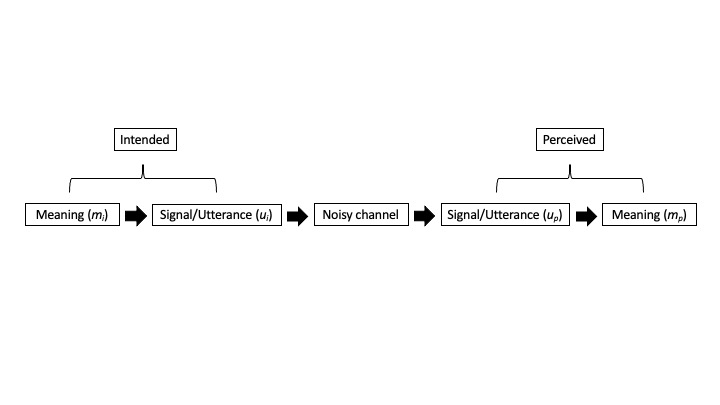
\includegraphics[width=0.9\linewidth]{figures/materials/noisy-channel} 

}

\caption{Schematic representation of the noisy channel model of communication}\label{fig:noisy-channel}
\end{figure}

The speaker produces an utterance \(u_i\) with a meaning \(m_i\) that she intends to send.
The utterance is encoded into a signal and is sent through a channel of transmission.
During transmission, some external noise disrupts the signal.
The receiver (e.g., a listener) perceives the signal as \(u_p\) and decodes it to recover the meaning as \(m_p\).
The human language comprehension system is assumed to be engaged in an optimal Bayesian decoding that uses all the sources of information
(e.g., a prior semantic knowledge, context information, world knowledge, etc.)
and infers the intended meaning from the perceived utterance that it receives from a noisy channel of communication (\protect\hyperlink{ref-Gibson2013}{Gibson et al., 2013}; \protect\hyperlink{ref-Levy2008}{Levy, 2008}; cf. \protect\hyperlink{ref-Markman2011}{Markman \& Otto, 2011}).

For successful communication to take place, the message recovered by the listener must be approximately equal to the message intended to be sent by the speaker.
Let's take an example.
X sees a spherical object flying towards Y.
So, she intends to warn him about it: a ``spherical object which is played by two teams of 11 players each in a big playground'' is about to hit Y.
To convey this message, X utters BALL.
Due to an external noise, X's (i.e., the speaker's) utterance is distorted, so Y (i.e., the listener) perceives the utterance as HALL.
The listener then interprets that the speaker's message is intended to point him to the ``building where lectures take place in their university'' which they were trying to find.
(In this case of unsuccessful communication, or due to the listener wrongly identifying the intended message of the speaker, Y gets hit by a ball.)

We assume that the goal of a listener is to identify the message \(m_i\) that is most likely from the perceived utterance \(u_p\), taking into account the external noise (\(N\)), and the prior likelihood of the speaker uttering \(u_i\).
This can be formally expressed as:

\begin{align} \label{eq:noisy-channel2}
\hat{m_p} &= \mathop{\mathrm{argmax}}\limits_{m_p} P(m_p,u_p,N,u_i,m_i)
\end{align}

These sequence of events from the intended message \(m_i\) to the perceived message \(m_p\) can be graphically represented in a Bayesian network (\protect\hyperlink{ref-Bruineberg2021}{Bruineberg et al., 2021}; \protect\hyperlink{ref-Darwiche2010}{Darwiche, 2010}; \protect\hyperlink{ref-Pearl1985}{Pearl, 1985}) in Figure \ref{fig:bayesian-network} (cf.~Figure \ref{fig:noisy-channel}).

\begin{figure}[!htpb]

{\centering 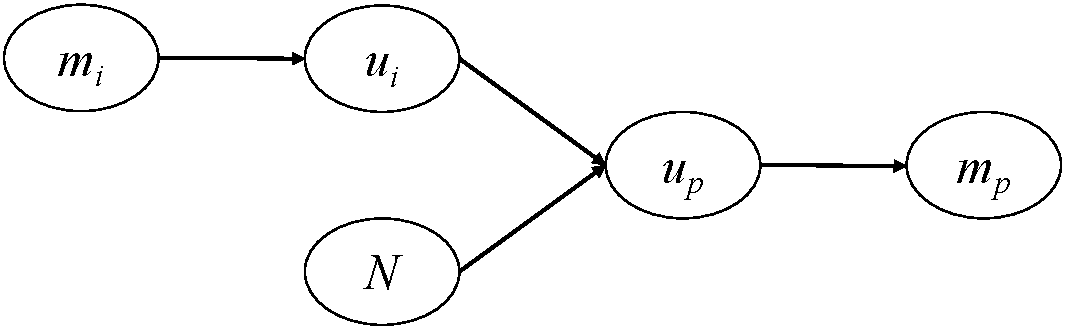
\includegraphics[width=0.9\linewidth]{figures/materials/bayesian-network} 

}

\caption{Bayesian network representation of the noisy channel model of communication}\label{fig:bayesian-network}
\end{figure}

Figure \ref{fig:bayesian-network} models the dependencies among the events,
which shows that the external noise and the speaker's utterance are \emph{independent},
however, the listener's perception of the uttered message is also dependent on the noise.
The communication in the noisy channel, represented as a Bayesian network, can now be expressed as:

\begin{align} \label{eq:noisy-channel3}
\hat{m_p} &= \mathop{\mathrm{argmax}}\limits_{m_p} P(m_p | u_p) * P(u_p|u_i, N) * P(u_i | m_i) * P(m_i)
\end{align}

Equation \eqref{eq:noisy-channel3} can be interpreted easily from its corresponding representation in Figure \ref{fig:bayesian-network}.

It shows:

\begin{itemize}
\tightlist
\item
  \(P(m_p | u_p)\): the probability of inferring a meaning \(m_p\) (e.g., a building where lectures take place) from a perceived utterance \(u_p\) (e.g.~/hall/)
\item
  \(P(u_p|u_i, N)\): bottom-up auditory information, i.e., the probability of the listener hearing a particular utterance \(u_p\) (e.g., /hall/) given that the speaker has uttered an utterance \(u_i\) (e.g., /ball/) in the noisy channel \(N\) (e.g., background noise, signal distortion, etc.)
\item
  \(P(u_i|m_i)P(m_i)\): prior information (e.g., top-down semantic knowledge, information about the speaker, etc.), i.e., the probability of a speaker uttering \(u_i\) with an intended message \(m_i\), and the marginal probability of the intended message \(m_i\)
\end{itemize}

The channel of transmission can become noisy due to factors like background noise present in a conversation,
a poor signal transmission of a telephone call that distorts the speaker's speech,
hearing loss of a listener,
hearing aid or cochlear implant worn by a listener, and so on.
To understand speech in such a noisy channel of communication, a listener puts different weights on the distorted bottom-up auditory input \(P(u_p|u_i, N)\) vs her prior information \(P(u_i|m_i)P(m_i)\) (e.g., knowledge about the speaker, world, context information, etc.).

Studies in clean speech comprehension and reading comprehension have demonstrated that listeners and readers use prior knowledge and context information to form semantic predictions about the linguistic events that are yet to be encountered.

Let's take the following sentence, for example:

\begin{enumerate}
\def\labelenumi{(\arabic{enumi})}
\tightlist
\item
  The day was breezy so the boy went outside to fly \ldots{}
\end{enumerate}

Most readers would expect the final words to be \emph{a kite} in this sentence (\protect\hyperlink{ref-Delong2005}{DeLong et al., 2005}; cf. \protect\hyperlink{ref-Nieuwland2020a}{Nieuwland et al., 2020}). Here, the words up to the final word of the sentence provide a context:
A reader can utilize their knowledge about what a \emph{boy} would ideally do \emph{outside} on a \emph{breezy} day.
It leads the reader to predict that the sentence continuation is most likely \emph{a kite} and not some improbable words like \emph{a rocket}.
Similar results are observed in the auditory domain as well.
Listeners use context information from what they have heard, and form predictions about an upcoming word (e.g., \protect\hyperlink{ref-Altmann2007}{Altmann \& Kamide, 2007}; \protect\hyperlink{ref-Ankener2019}{Ankener, 2019}).
That is, human language comprehension is predictive in nature such that listeners engage in predictive language processing (Section \ref{predictive-language-processing}, \protect\hyperlink{ref-Kuperberg2016}{Kuperberg \& Jaeger, 2016}; \protect\hyperlink{ref-Pickering2018}{Pickering \& Gambi, 2018}).
In a noisy channel, listeners' engagement in predictive processing is influenced by the noise in the signal (\protect\hyperlink{ref-Obleser2007}{Obleser et al., 2007}; \protect\hyperlink{ref-Sheldon2008a}{Sheldon et al., 2008a}).

Based on the theoretical accounts of the noisy channel model of communication and the predictive language processing (\protect\hyperlink{ref-Christiansen2015}{Christiansen \& Chater, 2015}; \protect\hyperlink{ref-Ferreira2016}{Ferreira \& Lowder, 2016}; \protect\hyperlink{ref-Friston2020}{Friston, Parr, et al., 2020}; \protect\hyperlink{ref-Hale2001}{Hale, 2001}; \protect\hyperlink{ref-Levy2008}{Levy, 2008}; \protect\hyperlink{ref-Mcclelland1986}{McClelland \& Elman, 1986}; \protect\hyperlink{ref-Norris2016}{Norris et al., 2016}; \protect\hyperlink{ref-Pickering2018}{Pickering \& Gambi, 2018}),
this thesis investigates the interaction between top-down predictive and bottom-up auditory processes.
We examine how top-down predictive processes facilitate language comprehension in a noisy channel that is created by \protect\hyperlink{speech-processing}{acoustic degradation of speech}.
We examine the nature of predictability effects in a noisy channel.
We investigate what the optimal level of noise in the signal is, i.e., the optimal level of speech degradation,
for the effect of top-down predictive processes to be most efficient or facilitatory for language comprehension.
By manipulating different factors of top-down as well as bottom-up processes (e.g., speech rates, attention allocation to different parts of the speech stream),
we examine their role in aiding or interfering with the comprehension of degraded speech.
While doing so, we address the following research goals.

\hypertarget{research-goals}{%
\section{Research goals}\label{research-goals}}

\begin{enumerate}
\def\labelenumi{(\arabic{enumi})}
\item
  \textbf{Replication of the predictability effect in a noisy channel}\\
  Almost all the disciplines of cognitive science --- anthropology, computer science, linguistics, neuroscience, and psychology --- are suffering the so-called replication crisis (\protect\hyperlink{ref-OSC2015}{Aarts et al., 2015}; \protect\hyperlink{ref-Cockburn2020}{Cockburn et al., 2020}; \protect\hyperlink{ref-Ebersole2016}{Ebersole et al., 2016}; \protect\hyperlink{ref-Minocher2021}{Minocher et al., 2021}; \protect\hyperlink{ref-Sanderson2008}{Sanderson \& Roberts, 2008}).
  The results of an experiment do not hold up consistently when conducted again by another group of researchers.
  For example, in a multi-lab collaborative study, Nieuwland et al. (\protect\hyperlink{ref-Nieuwland2020a}{2020}) did not find the same N400 effect at English articles (a/an) that DeLong et al. (\protect\hyperlink{ref-Delong2005}{2005}) had reported 15 years earlier.
  The first goal of this thesis is to test if we can replicate the facilitatory effect of semantic predictability in language comprehension in a noisy channel (e.g., \protect\hyperlink{ref-Obleser2007}{Obleser et al., 2007}; \protect\hyperlink{ref-Sheldon2008a}{Sheldon et al., 2008a}).
  Replication of the predictability effect in comprehension of degraded speech
  will help garner evidence in the favor of this \emph{effect of interest}.
  It will also provide a reliable foundation to test if (and how) other factors (e.g., speed of information processing) influence and interact with the facilitatory effect of predictability.
\item
  \textbf{Nature of prediction}\\
  There are at least two schools of thought which argue that prediction is either all-or-nothing or probabilistic in nature (\protect\hyperlink{ref-Coltheart2004}{Coltheart, 2004}; \protect\hyperlink{ref-Kuperberg2016}{Kuperberg \& Jaeger, 2016}; \protect\hyperlink{ref-Luke2016}{Luke \& Christianson, 2016}).
  These debates are, however, centered around reading comprehension and clean speech comprehension.
  The discussion about the nature of prediction in a noisy channel like degraded speech is sparse.
  Specifically, in degraded speech comprehension, only one study has empirically investigated the theoretical postulation that prediction is restricted only for highly predictable sentence endings (\protect\hyperlink{ref-Strauss2013}{Strauß et al., 2013}).
  Therefore, the second goal of this thesis is to examine the nature of the predictability effect.
  With carefully designed experiments and materials, this thesis aims to test the distinction between all-or-nothing and probabilistic predictions in degraded speech comprehension.
\item
  \textbf{Boundary conditions of predictive language processing}\\
  Several authors claim that predictive processing is the fundamental nature of human cognition, and thus, by definition, also of language processing (\protect\hyperlink{ref-Clark2013}{A. Clark, 2013}; \protect\hyperlink{ref-Friston2020}{Friston, Parr, et al., 2020}; \protect\hyperlink{ref-Friston2020b}{Friston, Sajid, et al., 2020}; \protect\hyperlink{ref-Kuperberg2020}{Kuperberg, 2021}; \protect\hyperlink{ref-Lupyan2015}{Lupyan \& Clark, 2015}).
  At the same time, an increasing number of studies are showing boundary conditions as well as prerequisite conditions for predictive language processing (\protect\hyperlink{ref-Federmeier2010}{K. D. Federmeier et al., 2010}; \protect\hyperlink{ref-Huettig2019}{Huettig \& Guerra, 2019}; \protect\hyperlink{ref-Huettig2016}{Huettig \& Mani, 2016}; \protect\hyperlink{ref-Mishra2012}{Mishra et al., 2012}).
  For example, attention can reverse the effect of predictability in non-speech auditory perception (cf. \protect\hyperlink{ref-Kok2012}{Kok et al., 2012}).
  In a noisy channel (i.e., degraded speech), attention to a part or parts of a speech stream can modulate or the limit predictability effect as different parts of the speech stream contain different linguistic units;
  each linguist unit (e.g., each word in a sentence) carries its own meaning that serves the entire message (e.g., the entire sentence).
  Therefore, the third goal of this thesis is to examine the role of auditory attention that can act as a prerequisite for semantic predictions,
  or limit the automaticity of predictive processing in degraded speech comprehension.\\
  This thesis aims to test whether attention to different parts of degraded speech stream aids, or hampers facilitatory effects of top-down predictions.
\item
  \textbf{Adaptation to degraded speech}\\
  Despite the difficulty in understanding speech in a noisy channel,
  listeners rapidly adapt to degraded speech (\protect\hyperlink{ref-Rosen1999}{Rosen et al., 1999}).
  When the properties of speech vary in the dimension of both acoustic-phonetic cues as well as lexical-semantic cues,
  adaptation can be difficult.
  The fourth goal of this thesis is to examine if listeners adapt to degraded speech when both degradation level and predictability of speech are varied.
  We test if an adaptation to the bottom-up perceptual property of speech is influenced by its top-down semantic property.
\item
  \textbf{Speed of information processing}\\
  Unlike visual scene which opens in spatial dimension, speech signal flows in temporal dimension.
  This poses a challenge to the listeners to process information at different speed and timescales when
  more time is available to process the information in slow speech while less time is available for fast speech (\protect\hyperlink{ref-Lerner2014}{Lerner et al., 2014}).
  Listeners build up the meaning representation as they process the speech to predict upcoming linguistic unit.
  The fifth goal of this thesis is to examine whether a change in information flow, i.e., speech rate, affects facilitatory effect of predictability.
  We test if an increase or decrease in speech rate impedes the intelligibility of speech over a noisy channel,
  and whether it impedes or further aids the predictability effect in the noisy channel.
\item
  \textbf{Metric for measurement of language comprehension}\\
  In the study of speech perception and language comprehension, different researchers have used different measurement metrics (\protect\hyperlink{ref-Amichetti2018}{Amichetti et al., 2018}; \protect\hyperlink{ref-Obleser2007}{Obleser et al., 2007}; \protect\hyperlink{ref-Peelle2013}{Peelle, 2013}; \protect\hyperlink{ref-Sheldon2008a}{Sheldon et al., 2008a}).
  The measurement is inconsistent across studies which becomes a problem especially when the effect of context in comprehension is under discussion:
  cross-study comparison does not give a clear picture of the predictability effect in this case.
  Therefore, the sixth goal of this thesis is to establish and consistently use a sensitive metric for the measurement of language comprehension that takes into account whether participants (in)correctly use the context-evoking word in a sentence.
\end{enumerate}

Studies addressing the research goals outlined above will primarily contribute to elaborating and developing the existing theories of predictive language processing, and furthering the understanding of spoken language comprehension in a noisy channel, especially degraded speech comprehension.
Below we present the contributions of the research presented in this thesis.

\hypertarget{research-contributions}{%
\section{Research contributions}\label{research-contributions}}

The research reported in this thesis examines theoretical questions of predictive language processing and its boundary conditions when spoken language comprehension takes place through a noisy channel.
It contributes to the studies of speech perception, language comprehension, predictive coding, language science, audiology, psycholinguistics, psychology, and broadly to cognitive science.
In an applied setup, this informs translational/clinical researchers about language comprehension in \protect\hyperlink{distortion-degradation}{cochlear implantees}.

\begin{itemize}
\item
  \textbf{Graded effect of predictability}\\
  We replicate the previous finding of the predictability effect showing that predictability facilitates comprehension of degraded speech at moderate levels of degradation.
  Additionally, in the existing debate of all-or-nothing vs graded prediction, our findings indicate that prediction across the noisy channel of degraded speech is graded in nature
  rather than being restricted to a narrow space of highly predictable sentence endings.
  Goals 1 and 2 correspond to this research contribution which is brought about by the experiments described in Chapters \ref{chapter-attention-prediction} and \ref{chapter-graded-prediction}.
\item
  \textbf{Attention in predictive language processing}\\
  We show that predictive processing is not always automatic and it cannot all by itself cannot explain how listeners understand speech in a noisy channel.
  Although top-down predictions facilitate comprehension, we show that attention to the context is a prerequisite for such contextual facilitation.
  Only when listeners attend to the context information and form its meaning representation, then the top-down predictions can facilitate comprehension of degraded speech.
  Without proper attention to the context, predictability effects cannot be observed.
  Goal 3 corresponds to this research contribution which is brought about by the experiment described in Chapter \ref{chapter-attention-prediction}.
\item
  \textbf{Absence of perceptual adaptation}\\
  We show that listeners do not adapt to degraded speech when lexical-semantic cues are taken into consideration.
  This is in contrast with the previous findings of speech perception experiments some of which disregard the trial-by-trial variation in sentence context (e.g., \protect\hyperlink{ref-Davis2005}{Davis et al., 2005}; \protect\hyperlink{ref-Erb2013}{Erb et al., 2013}).
  When listeners are engaged in a linguistic task in which the lexical cues vary on every trial,
  their cognitive resources are strained by lexical-semantic cues rather than acoustic-phonetic cues.
  Thus, they do not show any adaptation effect;
  every trial is effectively a novel trial for them.
  Goal 4 corresponds to this research contribution which is brought about by the experiment described mainly in Chapter \ref{chapter-graded-prediction}, and in Chapter \ref{chapter-speech-rate}.
\item
  \textbf{Change in information flow and its effect on top-down prediction}\\
  We show that different rates of information flow --- increase or decrease in the rate of speech --- have different effects on language comprehension.
  Intelligibility of speech decreases with both increase and decrease of speech rate.
  But the increase in speech rate is particularly detrimental to comprehension of degraded speech as it increases the difficulty in processing sentences with less predictable endings.
  This is one of the very few studies highlighting the role of speed of flow of information in the contextual facilitation of degraded speech.
  Goal 5 corresponds to this research contribution which is brought about by the experiment described in Chapter \ref{chapter-speech-rate}.
\item
  \textbf{A metric of language comprehension}\\
  We propose and successfully use a metric of language comprehension that reflects listeners' use of context information.
  This metric does not merely measure how many words are correctly identified.
  Rather, it considers the fact that in the study of effect of predictability, how well a context is recognized should also be taken into account.
  Thus it measures word recognition accuracy in the sentences in which context is correctly recognized.
  The use of such a metric improves interpretation of contextual facilitation across studies, which lacks in the extant literature.
  Goal 6 corresponds to this research contribution which is brought about by consistent use of this metric in Chapters \ref{chapter-graded-prediction} and \ref{chapter-speech-rate}.
\end{itemize}

\hypertarget{overview-of-the-thesis}{%
\section{Overview of the thesis}\label{overview-of-the-thesis}}

The central theme of this thesis is the study of predictive processing in the process of language comprehension across a noisy channel.
On the grounds of predictive language processing and the noisy channel model of communication,
we investigate how and to what extent listeners use context information while listening to degraded speech.
We replicate and extend some prior findings claiming that at moderate levels of speech degradation,
predictability facilitates language comprehension.
We further examine the boundary conditions of predictive processing and examine how different rates of information flow moderate predictability effects.
We test for the presence of perceptual adaptation and find evidence against the learning effect and adaptation to degraded speech.

\noindent
\textbf{Chapter \ref{chapter-background}} provides a background on the rest of the chapters.
It provides an overview of degraded speech comprehension and predictive language processing.
The current status of the debate on these topics is also presented.

\noindent
\textbf{Chapter \ref{chapter-methods}} describes the stimuli used in all the experiments in this thesis.
It describes the process of stimuli creation, and speech processing, and also provides an overview of online data collection.

\noindent
\textbf{Chapter \ref{chapter-stats}} describes the statistical tests employed for data analyses.
Binomial logistic mixed effects modeling is performed on the data from all the experiments.
This chapter provides a background on this statistical procedure,
and how it is operated on the statistical software \texttt{R}.

\noindent
\textbf{Chapter \ref{chapter-attention-prediction}} presents two experiments that address the first and the third research goal.
These experiments are conducted to examine the predictability effect in degraded speech comprehension,
and the role of auditory attention in it.
Participants in both the experiments are presented with the speech degraded at different levels of degradation
and sentences of different levels of predictability.
Participants in Experiment 1A are asked to type in only the final word of a sentence;
this does not bind their attention to the sentence context.
While the participants in Experiment 1B are asked to type in the entire sentence that they heard which required them to attend to the sentence context as well.
We replicate the previously reported predictability effects in the noisy channel only when participants attended to the entire sentence including the context.
We show that at moderate levels of degradation, top-down predictions cannot be generated when insufficient attention is given to context.
We discuss the limitation in the theories of predictive language processing committing automaticity of prediction,
and argue the importance of incorporating \emph{attention} into current theories.
We end this chapter with the note that the measurement of language comprehension can be further refined,
and the nature of the predictability effect tested.

\noindent
\textbf{Chapter \ref{chapter-graded-prediction}} addresses the first, the second, the fourth, and the sixth research goals.
The predictability effect partially replicated in Chapter \ref{chapter-attention-prediction} is further examined in this chapter.
We use a refined metric of measurement of language comprehension that takes into consideration whether listeners correctly identified the context.
We observe predictability effects at a moderate level of speech degradation, thereby consistently replicating the facilitatory effect of predictability.
We find the predictability effects to be graded in nature,
and discuss it in the light of existing theories of predictive processing.
We also show that regardless of the certainty about the next-trial degradation level,
listeners do not adapt to degraded speech as its lexical-semantic property varies every trial.
At the end of this chapter, we note the intrinsic difficulty of processing degraded speech, and open the question that the predictability effects could be further enhanced (or limited) with more (or less) time available to process the degraded speech.

\noindent
\textbf{Chapter \ref{chapter-speech-rate}} addresses the questions opened in Chapter \ref{chapter-graded-prediction}.
In two experiments, it addresses the fourth, the fifth, and the sixth research goals.
We use the same metric of measurement of language comprehension as Chapter \ref{chapter-graded-prediction}, which takes into account listeners' correct identification of the context.
Listeners are presented with a moderately degraded speech at which the predictability effect is observed in Chapter \ref{chapter-graded-prediction}.
In Experiment 7A, the moderately degraded speech is presented at normal and fast speech rates.
And in Experiment 7B, the speech rates are normal and slow.
For fast speech, however, both intelligibility, as well as the predictability effect, are reduced which is driven by the difficulty in processing words that are less predictable from the context.
And although more time is available to process the context of the degraded speech at a slow speech rate,
there is no increase in the facilitatory effect of predictability with a reduced speech rate;
instead, intelligibility is reduced in slow speech compared to normal speech.
This chapter ends with a discussion on the limitations of predictive processing that are driven by the constraints in cognitive resources.

\noindent
\textbf{Chapter \ref{chapter-conclusion}} summarizes the findings of all the studies.
It presents the theoretical implications of this thesis and the future direction it points to.
The general limitations of the studies are briefly discussed.

\noindent
\textbf{Chapter \ref{chapter-ethics}} presents ethical approval that was obtained to run the experiments on the human subjects.
The source that provided funding to conduct the research presented in this thesis is disclosed.

\hypertarget{dissimination-of-research-findings}{%
\section{Dissimination of research findings}\label{dissimination-of-research-findings}}

Some of the findings reported in this thesis are presented and published, in part, elsewhere as a means of dissemination of scientific findings.
The list of presentations and publications that report on parts of the research described in this thesis is outlined below.

\begin{itemize}
\item
  Bhandari, P., Demberg, V., \& Kray, J.
  (\emph{in preparation}) Speaking fast and slow: How speech rate affects contextual facilitation in degraded speech comprehension.
\item
  Bhandari, P., Demberg, V., \& Kray, J.
  (\emph{under review}) Predictability effects in degraded speech comprehension are reduced as a function of attention.
\item
  Bhandari, P., Demberg, V., \& Kray, J.
  (2022).
  The effect of speech rate in comprehension of degraded speech.
  \emph{International Max Planck Research School (IMPRS) Conference}, 2022-06-01--2022-06-03.
\item
  Bhandari, P., Demberg, V., \& Kray, J.
  (2022).
  Predictability effects are reduced as a function of attention.
  \emph{Annual Convention of American Psychological Association}, 2022-05-25--2022-05-28.
\item
  Bhandari, P., Demberg, V., \& Kray, J.
  (2021).
  Semantic predictability facilitates comprehension of degraded speech in a graded manner.
  \emph{Frontiers in Psychology}, \emph{12}, 714485.
\item
  Bhandari, P., Demberg, V., \& Kray, J.
  (2021).
  Predictability facilitates comprehension but not adaptation to degraded speech in a graded manner.
  \emph{Conference of the Society for the Neurobiology of Language}, 2021-10-05--2021-10-08.
\end{itemize}

\begin{itemize}
\tightlist
\item
  Bhandari, P., Demberg, V., \& Kray, J. (2021). Predictability facilitates comprehension of degraded speech in a graded manner. \emph{Annual Meeting of Cognitive Neuroscience Society}, 2021-03-13--2021-03-16.
\end{itemize}

\hypertarget{chapter-background}{%
\chapter{Background}\label{chapter-background}}

In the previous chapter, we outlined the theoretical background and the research goals of the studies in this dissertation.
We stated that the central theme of this thesis is to investigate the interaction between top-down predictive processes and bottom-up auditory processes in language comprehension.
Grounding on the noisy channel model of communication and predictive language processing,
the studies in this thesis manipulate the auditory processes \(P(u_p|u_i,N)\), and prior information \(P(u_i,m_i)\) in the form of semantic context available in a sentence.
In this chapter, we provide background on the noisy channel that was created and used to introduce variations in bottom-up processing in the studies presented in this thesis.
We also elaborate on the predictive language processing in the noisy channel, and the evidence of its limits and nature.
Understanding these fundamental concepts of top-down and bottom-up processes is essential for the chapters that follow;
these concepts are briefly reiterated in the following chapters wherever relevant.
Additionally, in this chapter we outline the gaps in previous research that this thesis fills in.

\hypertarget{distortion-degradation}{%
\section{Speech distortion and degradation}\label{distortion-degradation}}

In an ideal situation, speech perception is a seamless process: a speaker produces an utterance, the speech signal transmits via a medium like air, and a listener perceives the signal as the speech waves enter her ears initiating a cascade of mechanical-neural processes of audition.
However, speech perception is hardly as smooth as it seems.
As shown in Figure \ref{fig:noisy-channel} and Equation \eqref{eq:noisy-channel3}, in the noisy channel model of communication (\protect\hyperlink{ref-Gibson2013}{Gibson et al., 2013}, \protect\hyperlink{ref-Gibson2019}{2019}; \protect\hyperlink{ref-Levy2008}{Levy, 2008}; \protect\hyperlink{ref-Shannon1948}{C. E. Shannon, 1948}),
noise disrupts and distorts the speech signal \(u_i\) uttered by a speaker
which the listener then perceives as \(u_p\) and decodes into the message \(m_p\).
Distortion can occur at these three points or sources: encoding, transmission, and decoding.
Speech can be distorted while encoding the utterance \(u_i\) due to the variability in speakers' production, like accented speech, or soft and rapid speech.
Distortion can arise while decoding the signal \(u_p\) due to listener-related factors, like hearing loss, or auditory processing disorder.
It can also be a result of the noise that appears during the transmission, like ambient noise, or poor medium of transmission (e.g., distortion in the telephone line).
All these sources of distortion make the listening condition adverse (\protect\hyperlink{ref-Mattys2012}{Mattys et al., 2012}) by affecting the time and frequency related properties/cues of the speech signal, i.e., temporal envelope cues and spectral details of speech respectively.
The temporal envelope cues are the slow variations in the amplitude of the speech signal over time (\protect\hyperlink{ref-Moon2014}{Moon et al., 2014}; \protect\hyperlink{ref-Moon2014a}{Moon \& Hong, 2014}) while the spectral details are the frequency specific information about the speech.
The temporal envelope cues reflect the prosodic information of the speech, and are used in the lexical-semantic and syntactic processing (\protect\hyperlink{ref-Greenberg1996}{Greenberg, 1996}; \protect\hyperlink{ref-Schneider2001}{Schneider \& Pichora-Fuller, 2001}; \protect\hyperlink{ref-Sheldon2008b}{Sheldon et al., 2008b}).
The spectral details provide information about the sound production reflecting the resonant properties of the vocal tract, frequency range of the speech signal, energy distribution across frequency bands, etc. (\protect\hyperlink{ref-Roberts2011}{Roberts et al., 2011}; \protect\hyperlink{ref-Shannon1995}{Shannon et al., 1995}; \protect\hyperlink{ref-Shannon2004}{Shannon et al., 2004}).

In an experimental setup, a noisy channel can be created artificially by digital signal processing (see Section \ref{speech-processing}) to investigate the response of the speech perception system to the distorted speech
and to study language comprehension in an adverse listening condition.
For example, expansion or compression of speech signal acts upon the temporal property of the speech and makes it slow or fast, and an optimal level of speech expansion/compression does not distort the spectral property of speech (see Section \ref{compression-expansion}).
In addition to speech compression and expansion in Chapter \ref{chapter-speech-rate},
throughout the studies in this thesis, we implement noise vocoding to manipulate the spectral property of speech and create a noisy channel of communication.

Noise vocoding removes the spectral details of the speech signal in a controlled manner only leaving intact its temporal and periodicity cues (see Section \ref{noise-vocoding}).
This method of speech degradation was initially developed as a means to reduce the information in speech signal to be transmitted through the telephone line (\protect\hyperlink{ref-Vocoder1940}{Clendeninn, 1940}; \protect\hyperlink{ref-Dudley1939}{Dudley, 1939}).
Shannon and colleagues later modified and used this technique as an analogue to cochlear implant such that number of channels used in a cochlear implant are similar to the number of noise vocoding channels in terms of their speech output and intelligibility (\protect\hyperlink{ref-Loizou1999}{Loizou et al., 1999}; \protect\hyperlink{ref-Shannon1995}{Shannon et al., 1995}; \protect\hyperlink{ref-Shannon2004}{Shannon et al., 2004}; cf. \protect\hyperlink{ref-Orena2021}{Orena \& Colby, 2021}).
Therefore, in addition to being a method of speech distortion to parametrically vary and control the quality of speech signal in a graded manner,
noise vocoding is also a method of distortion that is used to understand the speech perception and language comprehension in cochlear implantees (e.g., \protect\hyperlink{ref-Patro2020}{Patro \& Mendel, 2020}; \protect\hyperlink{ref-Shannon2004}{Shannon et al., 2004}; \protect\hyperlink{ref-Winn2016}{M. Winn, 2016})

One of the main factors that determines the intelligibility of degraded speech is the number of noise vocoding channels.\footnote{Throughout this thesis, speech distortion by noise vocoding is referred to as speech degradation, or spectral degradation of speech.}
The higher the number of noise vocoding channels, the more is the frequency specific information available in the degraded speech,
consequently, higher is the intelligibility compared to the speech that is degraded with lesser number of noise vocoding channels.
For example, listeners are shown to rate 8 channels noise vocoded speech to be more intelligible and less effortful compared to 2 channels noise vocoded speech (e.g., \protect\hyperlink{ref-Obleser2011}{Obleser \& Kotz, 2011}; \protect\hyperlink{ref-Sohoglu2012}{Sohoglu et al., 2012}).
In our studies, we create noisy channel of different levels of degradation and intelligibility by noise vocoding the speech signal through 1, 4, 6 and 8 channels.
The details of the artificial distortions are described in Chapter \ref{chapter-methods}.

\hypertarget{prediction-and-comprehension-of-degraded-speech}{%
\section{Prediction and comprehension of degraded speech}\label{prediction-and-comprehension-of-degraded-speech}}

In addition to the quality of speech signal, listeners rely also on the context information and form top-down predictions to understand speech in adverse listening condition.
Below, we first review the role of predictions in language comprehension in general,
then we discuss the role of top-down predictive processes in comprehension of degraded speech in particular.

\hypertarget{predictive-language-processing}{%
\subsection{Predictive language processing}\label{predictive-language-processing}}

Research from various domains of cognitive (neuro)science, like emotion, vision, odor, and proprioception (the sensation of one's body position and movement, \protect\hyperlink{ref-Tuthill2018}{Tuthill \& Azim, 2018}), has shown that perception and cognition can be described under the framework of predictive processing; they primarily operate by predicting upcoming events (\protect\hyperlink{ref-Clark2013}{A. Clark, 2013}; \protect\hyperlink{ref-Marques2018}{Marques et al., 2018}; \protect\hyperlink{ref-Seth2013}{Seth, 2013}; \protect\hyperlink{ref-Stadler2012}{Stadler et al., 2012}; cf. \protect\hyperlink{ref-Bowers2012}{Bowers \& Davis, 2012}; \protect\hyperlink{ref-Jones2011}{Jones \& Love, 2011}; \protect\hyperlink{ref-Pierce1987}{Pierce \& Ollason, 1987}).
Human language comprehension too has been claimed to be predictive in nature from as early as mid-twentieth century (e.g., \protect\hyperlink{ref-Mccullough1958}{McCullough, 1958}; \protect\hyperlink{ref-Miller1951}{Miller et al., 1951}; \protect\hyperlink{ref-Morton1964}{Morton, 1964})
which in recent days has received an overwhelming support from computational linguistics, psycholinguistics and cognitive neuroscience of language (e.g., \protect\hyperlink{ref-Delong2005}{DeLong et al., 2005}; \protect\hyperlink{ref-Demberg2013}{Demberg et al., 2013}; \protect\hyperlink{ref-Heyselaar2021}{Heyselaar et al., 2021}; \protect\hyperlink{ref-Lupyan2015}{Lupyan \& Clark, 2015}; \protect\hyperlink{ref-Pickering2018}{Pickering \& Gambi, 2018}).
Empirical evidence from a number of studies suggests that readers and listeners predict upcoming words in a sentence when the words are predictable from the preceding context (\protect\hyperlink{ref-Kuperberg2016}{Kuperberg \& Jaeger, 2016}; \protect\hyperlink{ref-Nieuwland2019}{Nieuwland, 2019}; for reviews, \protect\hyperlink{ref-Staub2015}{Staub, 2015}).
For instance, predictable words are skipped and read faster compared to the words that are less predictable from the context (\protect\hyperlink{ref-Ehrlich1981}{Ehrlich \& Rayner, 1981}; \protect\hyperlink{ref-Frisson2005}{Frisson et al., 2005}; \protect\hyperlink{ref-Staub2011}{Staub, 2011}).
Applying visual world paradigm, studies have demonstrated that individuals show anticipatory eye movements towards a picture of an object (e.g., \emph{cake}) that is predictable from the preceding sentence context (e.g., \emph{The boy will eat a\ldots{}}) even before hearing the final target word (\protect\hyperlink{ref-Altmann1999}{Altmann \& Kamide, 1999}; \protect\hyperlink{ref-Ankener2018}{Ankener et al., 2018}; \protect\hyperlink{ref-Kamide2003}{Kamide et al., 2003}).
Similar results have been observed in virtual world set-up with naturalistic scenes (e.g., \protect\hyperlink{ref-Heyselaar2021}{Heyselaar et al., 2021}).
The sentence-final word in a highly constraining sentence (e.g., \emph{``She dribbles a ball.''}) elicits a smaller N400 amplitude\footnote{N400 is a negative-going EEG component that peaks around 400 ms post-stimulus, and it is considered as a neural marker of context-based semantic unexpectedness (\protect\hyperlink{ref-Kutas2011}{Kutas \& Federmeier, 2011}).} than a less constraining sentence (e.g., \emph{``She buys a ball.''}, \protect\hyperlink{ref-Federmeier2007}{K. Federmeier et al., 2007}; \protect\hyperlink{ref-Kutas1984}{Kutas \& Hillyard, 1984}).
Similarly, event-related words (e.g., \emph{``luggage''}) elicited reduced N400 compared to event-unrelated words (e.g., \emph{``vegetables''}) which were not predictable from the context (e.g., in an event of \emph{``travel''}, \protect\hyperlink{ref-Metusalem2012}{Metusalem et al., 2012}).
In sum, as the sentence context builds up, listeners make predictions about upcoming words in the sentence, and these in turn facilitate language comprehension.
That is, individuals use the context available to them to generate predictions which aids understanding written and spoken language.

\hypertarget{background-facilitatory-effect}{%
\subsection{Facilitatory effect of predictability}\label{background-facilitatory-effect}}

We have discussed above that individuals make predictions about not-yet-encountered linguistic units based on available context information as a sentence unfolds:
Top-down predictive and bottom-up perceptual processes interact dynamically in language comprehension.
When the bottom-up perceptual input is less reliable, for example, in an adverse listening condition, it has been shown that listeners rely more on top-down processes by narrowing down the predictions to smaller sets of semantic categories or words (e.g., \protect\hyperlink{ref-Strauss2013}{Strauß et al., 2013}; see also \protect\hyperlink{ref-Corps2020}{Corps \& Rabagliati, 2020}).
Obleser and colleagues (\protect\hyperlink{ref-Obleser2007}{Obleser et al., 2007}; \protect\hyperlink{ref-Obleser2010}{Obleser \& Kotz, 2010}), for instance, used sentences of two levels of semantic predictability (high and low) and systematically degraded speech signal by passing it through various numbers of noise vocoding channels ranging from 1 to 32 in a series of behavioral and neuroimaging studies (see also \protect\hyperlink{ref-Hunter2018}{Hunter \& Pisoni, 2018}).
They found that semantic predictability facilitated language comprehension only at moderate levels of speech degradation.
That is, participants relied more on sentence context when the speech signal was degraded though \emph{intelligible enough}, than when it was not degraded, or when it was highly degraded.
At such moderate levels of speech degradation, accuracy of word recognition was found to be higher for words in high predictability sentences than the words in low predictability sentences (\protect\hyperlink{ref-Obleser2010}{Obleser \& Kotz, 2010}).
For the extremes, i.e., when the speech signal was highly degraded (making the speech almost completely unintelligible) or when it was the least degraded (rendering the speech intelligible),
the word recognition accuracy was similar across both levels of sentence predictability, meaning that predictability did not facilitate language comprehension.
Sheldon et al. (\protect\hyperlink{ref-Sheldon2008b}{2008b}) estimated that for both younger and older adults, the number of noise vocoding channels required to achieve 50\% accuracy varied as a function of sentence context.
To achieve the same level of accuracy as highly constraining sentences, a higher number of channels (i.e., more bottom-up information) was required in less constraining sentences.
They also concluded that when the speech is degraded, word recognition is facilitated by predictability and sentence context.
Taken together, these studies conclude that at moderate levels of degradation, participants rely more on the top-down predictions generated by a sentence context and less on the bottom-up perceptual processing of unclear, less reliable, and degraded speech signal (\protect\hyperlink{ref-Obleser2014}{Obleser, 2014}).
However, these studies are agnostic about the nature of prediction, i.e., if it is probabilistic or deterministic.

\hypertarget{nature-of-prediction}{%
\subsubsection{Nature of prediction}\label{nature-of-prediction}}

\noindent
A debate in the literature of predictive language processing pertains to this question: Is prediction probabilistic, or is it an all-or-nothing phenomenon?
For instance, garden path phenomenon was explained as a parser's irreversible prediction about the sentence structure
which if fails (or, if it turns out to be incorrect), then the parser reanalyzes the sentence, and reformulates another prediction (e.g., \protect\hyperlink{ref-Ferreira1986}{Ferreira \& Clifton Jr, 1986}; see also \protect\hyperlink{ref-Demberg2013}{Demberg et al., 2013}; \protect\hyperlink{ref-Slattery2013}{Slattery et al., 2013}).
In recent days, the support for the probabilistic nature of prediction comes, for example, from ERP studies that show an inverse and graded relationship between the magnitude of N400 effect evoked by a word and its predictability measured by cloze probability (e.g., \protect\hyperlink{ref-Delong2005}{DeLong et al., 2005}).
The correlation between a word's \emph{surprisal}\footnote{Surprisal is a measure of the change in probability mass (or simply put, the change in expectation) as predictions are proven wrong with an encounter of new words in a sentence, discourse, etc. (\protect\hyperlink{ref-Hale2001}{Hale, 2001}).} in its linguistic context and the processing effort associated with it also demonstrates the probabilistic nature of prediction (e.g., \protect\hyperlink{ref-Hale2001}{Hale, 2001}; \protect\hyperlink{ref-Smith2008}{Smith \& Levy, 2008}).

These discussions come from reading studies and spoken language comprehension in clear speech.
Although a few models of language processing speculate that language comprehension in adverse listening condition can be predictive (e.g., \protect\hyperlink{ref-Lowder2016}{Lowder \& Ferreira, 2016}; \protect\hyperlink{ref-Ryskin2018}{Ryskin et al., 2018}),
so far, only Strauß et al. (\protect\hyperlink{ref-Strauss2013}{2013}) have investigated the nature of prediction in degraded speech comprehension.
They proposed an ``expectancy searchlight model'' which suggests that listeners form \emph{narrowed expectations} from a restricted semantic space only when the sentence endings are highly predictable.
They rule out the graded nature of predictability.
However, their approach to predictability was confounded by verb-noun association
(discussed in Chapter \ref{chapter-graded-prediction}).
In contrast to their study, we systematically vary the predictability of target word,
and examine the graded vs.~probabilistic nature of prediction in degraded speech comprehension.
We argue that the facilitatory effect of predictability is graded in nature;
it is not an all-or-nothing phenomenon focused solely on highly predictable sentence endings.

\hypertarget{limits-of-pp}{%
\subsection{Limits of predictive language processing}\label{limits-of-pp}}

It is important to note and acknowledge that the ubiquity and universality of predictive language processing has not gone unquestioned (\protect\hyperlink{ref-Huettig2016}{Huettig \& Mani, 2016}).
Apart from the debate on the nature of prediction, which we will come to later in this chapter, there is compelling evidence that questions the necessity of prediction in language comprehension.
For example, Mishra et al. (\protect\hyperlink{ref-Mishra2012}{2012}) showed that literacy is a key factor that limits listeners' prediction about upcoming word.
In a visual word paradigm study, they found that individuals with lower literacy showed less anticipatory eye movements compared to the individuals with higher literacy.
They bolstered their finding in a neuroimaging study claiming that learning to read fundamentally changes the neural circuitry (\protect\hyperlink{ref-Hervais2019}{Hervais-Adelman et al., 2019}).
It is therefore plausible that such structural change in the brain is manifested in linguistic behavior.
Similarly, Scholman et al. (\protect\hyperlink{ref-Scholman2020}{2020}) demonstrated that literacy is predictive of readers' sensitivity to discourse signals available in the context for the prediction of upcoming content.
Cognitive aging has also been shown to be a limiting factor in generating predictions.
Smaller N400 amplitude and latency in older adults compared to younger adults have been shown as an evidence of inability of older adults to engage in predictive language processing.
Among older adults, those with lower working memory scores are shown to be further disadvantaged when it comes to the use of context information (\protect\hyperlink{ref-Federmeier2002}{K. Federmeier et al., 2002}; \protect\hyperlink{ref-Federmeier2010}{K. D. Federmeier et al., 2010}).
Another line of argument that critiques the predictive processing comes from the observations of Huettig \& Guerra (\protect\hyperlink{ref-Huettig2019}{2019}).
They analyzed participants' anticipatory eye movements in the visual world paradigm and showed that listeners predict the target word only in an \emph{artificial} set-up of long preview time coupled with slow speech (see also \protect\hyperlink{ref-Fernandez2020}{Fernandez et al., 2020}; cf. \protect\hyperlink{ref-Heyselaar2021}{Heyselaar et al., 2021}).

In this thesis, we study additional top-down and bottom-up processes that can interact with, and potentially limit the facilitatory effect of predictability.
For example, current theories of predictive processing are poor in explaining the role of \emph{attention} in semantic prediction (e.g., \protect\hyperlink{ref-Christiansen2015}{Christiansen \& Chater, 2015}; \protect\hyperlink{ref-Ferreira2016}{Ferreira \& Lowder, 2016}; \protect\hyperlink{ref-Pickering2018}{Pickering \& Gambi, 2018}; but see \protect\hyperlink{ref-Friston2020b}{Friston, Sajid, et al., 2020}).
We argue that attention to context information is critical in forming semantic predictions,
especially in degraded speech comprehension (cf. \protect\hyperlink{ref-Kok2012}{Kok et al., 2012}).
By manipulating listeners' attention allocation to parts of speech stream, we show that attention to context information is a pre-requisite for the listeners to generate predictions.
Similarly, from Pickering \& Gambi (\protect\hyperlink{ref-Pickering2018}{2018})'s \emph{prediction-by-production} account of predictive language processing,
it follows that comprehenders make predictions (about word-form) at a slow presentation rate, but not at a fast presentation rate.
However, the findings on the influence of speech rate on the facilitatory effect of predictability has been equivocal both in clear speech comprehension as well as in degraded speech comprehension (e.g., \protect\hyperlink{ref-Aydelott2004}{Aydelott \& Bates, 2004}; \protect\hyperlink{ref-Goy2013}{Goy et al., 2013}; \protect\hyperlink{ref-Iwasaki2002}{Iwasaki et al., 2002}; \protect\hyperlink{ref-Winn2021b}{M. B. Winn \& Teece, 2021}).
In this thesis, we investigate the effect of both fast and slow speech on the predictability effect in degraded speech comprehension.
We demonstrate that there is a scope for current theories of predictive language processing to` incorporate
the instances of varying predictability effects at fast and slow speech rate,
and the effects of attention in degraded speech comprehension.

\hypertarget{background-adaptation}{%
\section{Adaptation to degraded speech}\label{background-adaptation}}

Listeners quickly adapt to novel speech with artificial acoustic distortions (\protect\hyperlink{ref-Dupoux1997}{Dupoux \& Green, 1997}).
With a repeated exposure to distorted speech, listeners' comprehension improves over time (\protect\hyperlink{ref-Guediche2014}{Guediche et al., 2014}; for reviews, see \protect\hyperlink{ref-Samuel2009}{Samuel \& Kraljic, 2009}).
When the noise condition, like level of speech degradation is constant throughout the experiment, listeners adapt to it and the performance (e.g., word recognition) improves with as little as 20 minutes of exposure (\protect\hyperlink{ref-Rosen1999}{Rosen et al., 1999}).
For example, Davis et al. (\protect\hyperlink{ref-Davis2005}{2005}, Experiment 1) presented listeners with 6 channels noise vocoded speech and found an increase in the proportion of correctly reported words over the course of experiment.
Similarly, Erb et al. (\protect\hyperlink{ref-Erb2013}{2013}) presented participants with 4 channels noise vocoded speech and reached a similar conclusion.
In these experiments, only one speech degradation level (6 or 4 channels noise vocoded speech) was presented in one block.
There was no uncertainty about the next-trial speech degradation from the participants' perspective.
Additionally, semantic feature (i.e., target word predictability) was not varied.
When multiple types or levels of degraded speech signals are presented in a (pseudo-)randomized order within a block, then a listener is uncertain about the signal quality of any upcoming trial.
This can influence perceptual adaptation such that
it might be totally absent with the change in the characteristics of auditory signal throughout an experiment (\protect\hyperlink{ref-Mattys2012}{Mattys et al., 2012}).
In addition, trial-by-trial variability in the characteristics of distorted speech can impair word recognition (\protect\hyperlink{ref-Sommers1994}{Sommers et al., 1994}; see also \protect\hyperlink{ref-Dahan2006}{Dahan \& Magnuson, 2006}).
Only a limited number of studies has looked at how the (un)certainty about next-trial speech quality, and semantic feature influence adaptation.
For example, in a word-recognition task, Vaden et al. (\protect\hyperlink{ref-Vaden2013}{2013}) presented words at +3dB SNR and +10dB SNR in a pseudo-random order;
the goal was to minimize the certainty about the noise level within the block.
They proposed that an adaptive control system might be involved to optimize task the performance when the listeners are uncertain about an upcoming trial (\protect\hyperlink{ref-Eckert2016}{Eckert et al., 2016}; \protect\hyperlink{ref-Vaden2016}{Vaden Jr et al., 2016}; \protect\hyperlink{ref-Vaden2015}{Vaden et al., 2015}).
However, we cannot make a firm conclusion about perceptual adaptation \emph{per se} from their studies as they do not report the change in performance over the course of experiment.
Similarly, Obleser and colleagues (\protect\hyperlink{ref-Hartwigsen2015}{Hartwigsen et al., 2015}; \protect\hyperlink{ref-Obleser2007}{Obleser et al., 2007}; \protect\hyperlink{ref-Obleser2010}{Obleser \& Kotz, 2010}) also presented listeners with noise vocoded sentences (ranging from 2 to 32 channels noise vocoding) in a pseudo-randomized order but did not report the presence or absence of perceptual adaptation.
On the one hand, repeated exposure is shown to lead to perceptual adaptation to degraded speech.
On the other hand, uncertainty about the speech quality is speculated to impair word recognition.
Additionally, word-form predictions --- that the listeners are encouraged to make in the experiments reported in this thesis \footnote{The possibility of the absence of word-form prediction in the experiments in this thesis is discussed in Chapter \ref{chapter-speech-rate}.} --- are shown to be inefficient in facilitating adaptation to degraded speech (\protect\hyperlink{ref-Corps2020}{Corps \& Rabagliati, 2020}).
Therefore, we investigate the role of certainty about next-trial speech degradation level and its semantic property (i.e., target word predictability) in perceptual adaptation.
We argue that a trial-by-trial variation in higher level semantic feature of speech hinders listeners' perceptual system to retune itself to adapt to the lower level auditory features of the degraded speech (cf. \protect\hyperlink{ref-Nahum2008}{Nahum et al., 2008}).
In contrast to prior studies, we show that listeners do not adapt to degraded despite a repeated exposure to the same degraded speech
as long as its semantic predictability is uncertain.

\hypertarget{summary}{%
\section{Summary}\label{summary}}

In this chapter, we provided an overview of the concepts that will be repeated in the following chapters.
We introduced the concept of speech distortion and degradation.
Digital signal processing methods used in this process will be discussed in Chapter \ref{chapter-methods} (Section \ref{speech-processing}).
Importantly, we provided an overview of how predictive language processing aids language comprehension,
as well as its limitations.
We discussed perceptual adaptation to degraded speech, and the role of uncertainty about next-trial in adaptation.
At each step, we presented the motivation behind the studies in this thesis,
and the gaps in the literature these studies fill in.
In the next chapter, we will discuss the methods that are common in all the experiments (Chapters 5, 6, and 7) in developing materials and collecting data.

\hypertarget{chapter-methods}{%
\chapter{General methods}\label{chapter-methods}}

\chaptermark{Methods}

In this chapter we provide an overview of the experimental materials that are used in the experiments described in Chapters 5, 6, and 7.
Sentences used as experimental material were common to all the experiments,
and the signal processing method was also common.
Here, we also present an overview of online data collection.

\hypertarget{experimental-materials}{%
\section{Experimental materials}\label{experimental-materials}}

As a part of a study in the research project A4 of SFB1102, sentences of different levels of predictability were created.
Digital recordings of the sentences were degraded by noise vocoding and used in all experiments reported in this thesis.
Speech was also distorted by its compression and expansion.
Below we briefly describe how the sentences of different levels of predictability were obtained,
and what methodology was used to create distorted versions of the speech.

\hypertarget{stimulus-sentences}{%
\subsection{Stimulus sentences}\label{stimulus-sentences}}

With an aim to create sentences of three levels of predictability (low, medium, and high), a triplet of 120 sentences --- total of 360 sentences --- were created from 120 nouns.
Out of 120 nouns, 6 were repeated.
All sentences were in present tense consisting of pronoun, verb, determiner, and object.
These sentences were in Subject-Verb-Object form (e.g., \emph{Er fängt den Ball}. EN: He catches the ball.).
Some of these sentences were taken from Obleser \& Kotz (\protect\hyperlink{ref-Obleser2010}{2010}).
For each sentence, cloze probability ratings were collected from a group of young adults (n = 60; age range = 18 -- 30 years).
Mean cloze probabilities were 0.022 (SD = 0.027; range = 0.00 -- 0.09) for low-predictability sentences,
0.274 (SD = 0.134; range = 0.1 -- 0.55) for medium-predictability sentences,
and 0.752 (SD = 0.123; range = 0.56 -- 1.00) for high-predictability sentences.
The distribution of cloze probability across low-, medium-, and high-predictability sentences is shown in Figure \ref{fig:cloze-distribution},
and the cloze probability for individual sentence is shown in Appendix A.

\begin{figure}

{\centering 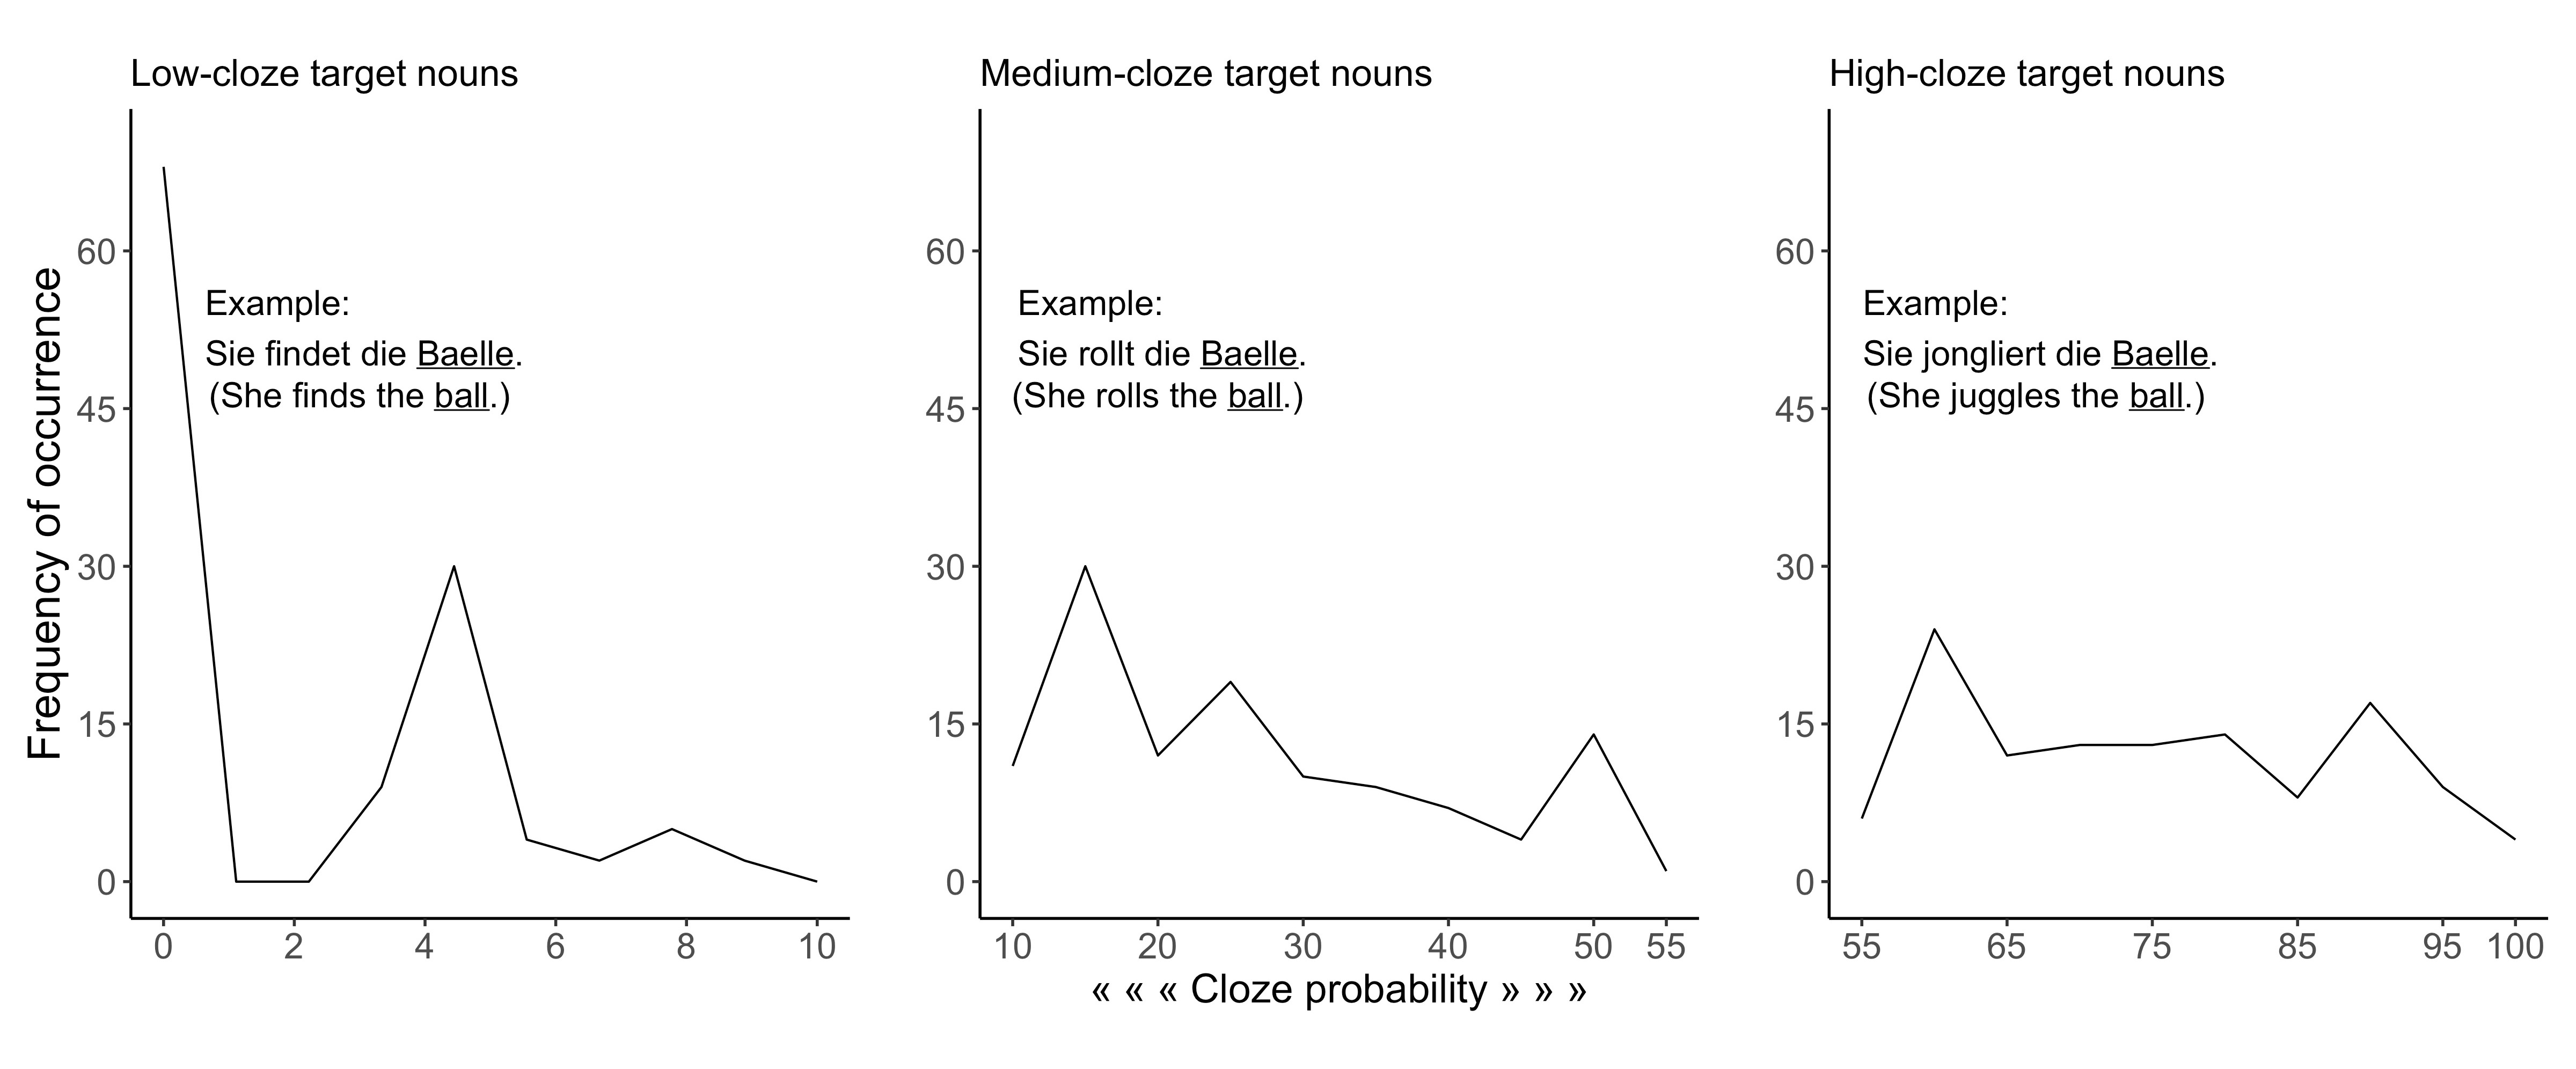
\includegraphics[width=0.9\linewidth]{figures/materials/cloze-distribution} 

}

\caption{Distribution of cloze probability ratings of target words in low, medium and high predictability sentences}\label{fig:cloze-distribution}
\end{figure}

\hypertarget{speech-processing}{%
\subsection{Speech processing}\label{speech-processing}}

All 360 sentence were spoken by a female native speaker of German at a normal rate.
The recordings were digitized at 44.1kHz with 32-bit linear encoding.
Spoken sentences used in Chapter 5, 6, 7, and 8 were degraded by noise vocoding.
In addition to degradation by noise vocoding, the sentences were distorted by compression and expansion of speech signal in Chapter 7.

\hypertarget{noise-vocoding}{%
\subsubsection{Noise-vocoding}\label{noise-vocoding}}

Noise vocoding is used to parametrically vary and control the quality of speech signal in a graded manner.
It distorts a speech signal by dividing it into specific frequency bands corresponding to the number of vocoder channels.
The frequency bands are analogous to the electrodes of cochlear implant (\protect\hyperlink{ref-Loizou1999}{Loizou et al., 1999}; \protect\hyperlink{ref-Shannon1995}{Shannon et al., 1995}; \protect\hyperlink{ref-Shannon2004}{Shannon et al., 2004}).
The amplitude envelope, i.e., the fluctuations of amplitude, within each frequency band is extracted and the spectral information within it is replaced by noise.
This makes the vocoded speech difficult to understand although temporal characteristics and periodicity of perceptual cues are preserved (\protect\hyperlink{ref-Rosen1999}{Rosen et al., 1999}).

The spectral degradation conditions of 1, 4, 6, and 8 channels were achieved for each of the 360 recorded sentences using a customized script originally written by Darwin (\protect\hyperlink{ref-Darwin2005}{2005}) in Praat software.
The speech signal was divided into 1, 4, 6, and 8 frequency bands between 70 and 9,000Hz.
The boundary frequencies were approximately logarithmically spaced following cochlear-frequency position functions (\protect\hyperlink{ref-Erb2014}{Erb, 2014}; \protect\hyperlink{ref-Greenwood1990}{Greenwood, 1990}; \protect\hyperlink{ref-Rosen1999}{Rosen et al., 1999}).
The amplitude envelope of each band was extracted and applied to band-pass filtered white noise in the same frequency ranges;
the upper and lower bounds for band extraction are specified in Table \ref{frequencies}.
Each of the modulated noise was then combined to produce degraded speech.
Scaling was performed to equate the root-mean-square value of the original undistorted speech and the final degraded speech.
This resulted into four levels of degradation: 1, 4, 6, and 8 channels noise vocoded speech.

Spectrograms of clear speech and noise-vocoded speech for the sentence \emph{Er löest die Aufgabe} are shown in Figure \ref{fig:vocoding-spectrogram}. It shows that with a decrease in the number of noise vocoding channels, the information in speech signal reduces and becomes noise-like.

\begin{figure}[!htpb]

{\centering 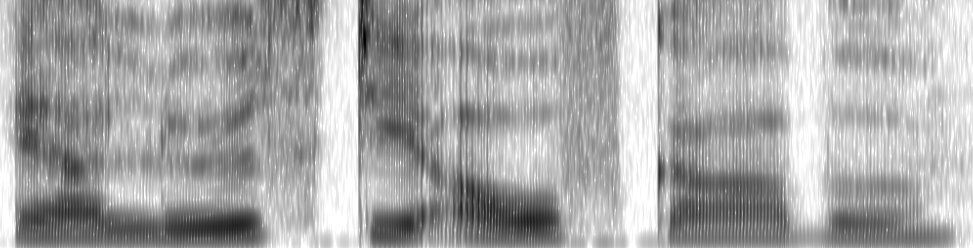
\includegraphics[width=0.9\linewidth]{figures/materials/aufgabe_clear} 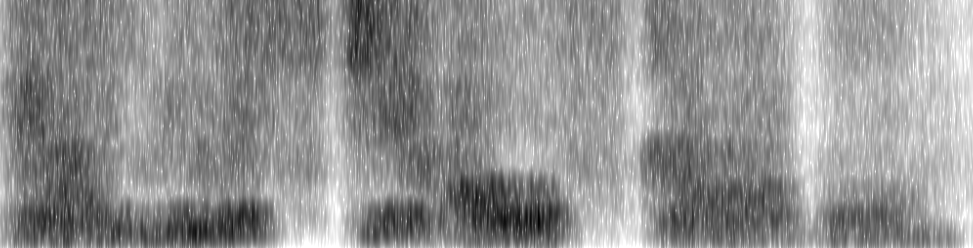
\includegraphics[width=0.9\linewidth]{figures/materials/aufgabe_8bands} 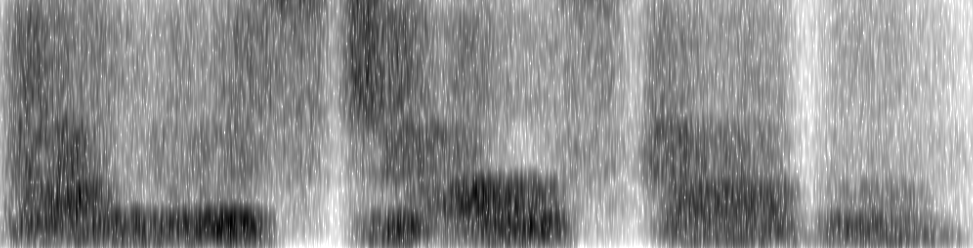
\includegraphics[width=0.9\linewidth]{figures/materials/aufgabe_6bands} 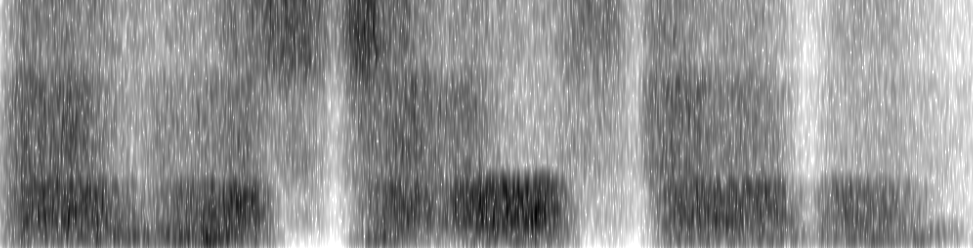
\includegraphics[width=0.9\linewidth]{figures/materials/aufgabe_4bands} 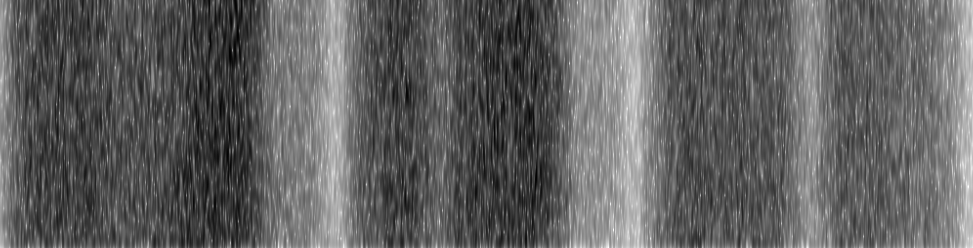
\includegraphics[width=0.9\linewidth]{figures/materials/aufgabe_1band} 

}

\caption{Spectrograms of clear speech, and degraded speech arranged with a decreasing number of noise vocoding channels (8, 6, 4 and 1 band) for the sentence `Er löest die Aufgabe.' }\label{fig:vocoding-spectrogram}
\end{figure}

\begin{table}[H]
\begin{center} 
\caption{Boundary frequencies (in Hz) for 1, 4, 6 and 8 channels noise-vocoding conditions} 
\label{frequencies} 
\vskip 0.12in
\begin{tabular}{llllllllll} 
\hline
Number of channels     &    Boundary frequencies \\
\hline
1   &   70    &   9000   &     &     &       &       &        &       &   \\

4   &   70    &   423   &   1304  &   3504  &   9000    &       &        &       &   \\

6   &   70    &   268   &   633   &   1304  &   2539    &   4813    &    9000    &       &   \\

8   &   70    &   207   &   423   &   764   &   1304    &   2156    &    3504    &   5634    &   9000\\
\hline
\end{tabular} 
\end{center} 
\end{table}

\hypertarget{compression-expansion}{%
\subsubsection{Speech compression and expansion}\label{compression-expansion}}

As early as the mid-twentieth century, investigators have reported that intelligibility does not drop significantly when speech is speeded up to 2 times the normal speech rate (e.g., \protect\hyperlink{ref-Garvey1953}{Garvey, 1953}).
Speech rate was increased by chopping physical tapes.
Digital algorithms like pitch-synchronous overlap-add technique (PSOLA, \protect\hyperlink{ref-Charpentier1986}{Charpentier \& Stella, 1986}; \protect\hyperlink{ref-Moulines1990}{Moulines \& Charpentier, 1990}) developed in the 1980s and later (overlap-add technique based on waveform similarity, \protect\hyperlink{ref-Verhelst1993}{Verhelst \& Roelands, 1993}) now allow us to speed up and slow down the speech rate in a controlled fashion.

In Chapter 7, we used Praat software that utilizes uniform time-compression algorithm (PSOLA) to create slow and fast speech with the compression factor of 1.35 and 0.65 respectively.
PSOLA analyzes the pitch of an auditory signal in the time domain of its digital waveform to set pitch marks, and then segments the signal into successive analysis windows centered around those pitch marks.
To create synthesized speech (i.e., fast or slow speech), a new set of pitch marks are calculated, and the analysis windows are rearranged.
Depending on the time-compression factor, some analysis windows are deleted, and the remaining windows are concatenated by superimposing and averaging the neighboring analysis windows.
The distortion of phonemic properties of speech signals are minimal when accelerating and slowing down within the range of factor 2 or below (\protect\hyperlink{ref-Moulines1990}{Moulines \& Charpentier, 1990}).

In Chapter 7, we created fast and slow versions of 120 high-predictability sentences and 120 low-predictability sentences, but did not use medium-predictability sentences.
These 480 recordings were then passed through 4 channels noise vocoding to use as experimental materials.

\hypertarget{data-collection-on-the-web}{%
\section{Data collection on the web}\label{data-collection-on-the-web}}

Traditionally, behavioral experiments with human participants are conducted in a laboratory setup.
In recent years, there has been a surge of experiments that are conducted on the web (\protect\hyperlink{ref-Reips2021}{Reips, 2021}).
The first generation of online experiments to study human cognition began in the mid 1990s (for reviews, \protect\hyperlink{ref-Musch2000}{Musch \& Reips, 2000}) with the advent of internet (\protect\hyperlink{ref-Bernerslee1992}{Berners-Lee et al., 1992}).
Welch \& Krantz (\protect\hyperlink{ref-Welch1996}{1996}) was the first online experiment that was conducted in 1995 as a part of tutorials in auditory perception (\protect\hyperlink{ref-Musch2000}{Musch \& Reips, 2000}).
In their survey of researchers, Musch \& Reips (\protect\hyperlink{ref-Musch2000}{2000}) discovered that until 2000, there were already at least 2 psycholinguistics experiments conducted online,
one of which studied the effect of context in shallow vs.~deep encoding of words.
Despite the difficulty in conducting online experiments, and skepticism of journals towards publishing results of online experiments,
Musch \& Reips (\protect\hyperlink{ref-Musch2000}{2000}) expressed optimism:

\begin{quote}
At the moment, the number of Web experiments is still small, but a rapid growth can be predicted on the basis of the present results.
We would not be surprised if within the next few years, a fair proportion of psychological experiments will be conducted on the Web. (\protect\hyperlink{ref-Musch2000}{Musch \& Reips, 2000, p. 85})
\end{quote}

And by 2021, there has been a significant growth in online experiments as technical and technological barriers are greatly reduced.
There are many software and online platforms which psychologists and psycholinguists can use with minimal knowledge of computer programming
to design, host and run their experiments, and retrieve these data in a fairly structured format (\protect\hyperlink{ref-Anwylirvine2020}{A. L. Anwyl-Irvine et al., 2020}; \protect\hyperlink{ref-Peirce2019}{Peirce et al., 2019}; \protect\hyperlink{ref-Prolific}{Prolific, 2014}; see also, \protect\hyperlink{ref-Anwylirvine2021}{A. Anwyl-Irvine et al., 2021}; \protect\hyperlink{ref-Eyal2021}{Eyal et al., 2021}).
Online experiments have demonstrated advantages over laboratory experiments (\protect\hyperlink{ref-Gadiraju2017}{Gadiraju et al., 2017}; \protect\hyperlink{ref-Johnson2021}{Johnson et al., 2021}).
For example, a large pool of participants is available online which is usually not possible in laboratory experiments.
Similarly, the participants in online experiments are more diverse than those in laboratory experiments.
Taking these advantages into consideration, psychologists and psycholinguists have conducted online experiments for almost 3 decades now.
Scientists who only conducted laboratory experiments, or who conducted online experiments only occasionally were forced to conduct their experiments almost exclusively on the web due to the restrictions imposed by covid-19 lockdown (\protect\hyperlink{ref-Gagne2021}{Gagné \& Franzen, 2021}; \protect\hyperlink{ref-Reips2021}{Reips, 2021}).
Since Welch \& Krantz (\protect\hyperlink{ref-Welch1996}{1996})'s auditory perception experiment, a number of experiments have been conducted online in auditory domain (\protect\hyperlink{ref-Leensen2013}{Leensen \& Dreschler, 2013}; \protect\hyperlink{ref-Seow2022}{Seow \& Hauser, 2022}; \protect\hyperlink{ref-vanOs2021}{van Os et al., 2021}; \protect\hyperlink{ref-Woods2017}{Woods et al., 2017}) replicating laboratory findings (e.g., \protect\hyperlink{ref-Cooke2021}{Cooke \& Garcia Lecumberri, 2021}).
The experiments reported in this thesis were also conducted online.

Initially, our experiments were designed to be conducted both in laboratory and online.
As the laboratory was shut down due to covid-19 pandemic-related lockdown (M. Schmitt, personal communication, March 16, 2020), we moved the laboratory experiments to the online platform.
We recruited participants online via Prolific Academic (\protect\hyperlink{ref-Prolific}{Prolific, 2014}).
We used Prolific's filters to recruit only native speakers of German residing in Germany
who reported to not have had any hearing loss, speech-language disorder, and cognitive impairment.
Participants were redirected to the experiments that were designed and hosted in Lingoturk (\protect\hyperlink{ref-Pusse2016}{Pusse et al., 2016}).
Lingoturk is a local hosting platform that manages crowdsourcing experiments --- it runs the experiments and stores the data.
We report the details of each experiment in Chapters 5, 6, and 7.

\hypertarget{chapter-stats}{%
\chapter{General statistical approach}\label{chapter-stats}}

\chaptermark{Statistics}

\hypertarget{linear-mixed-effects-models}{%
\section{Linear mixed effects models}\label{linear-mixed-effects-models}}

Linear mixed effects model (LME), as the name suggests, is a linear regression model that consists of both fixed effects and random effects.
It allows to model the underlying structure of the data which includes
the standard fixed effects like the levels of speech degradation and the levels of target word predictability
as well as random effects like items and participants.
These random effects are assumed to be random samples drawn from the general population.
In this thesis, the dependent variable (or an \emph{outcome}, or a \emph{response} variable) is binary (correct vs incorrect response).
So, we use binomial logistic mixed effects models with crossed random effects to model the data (\protect\hyperlink{ref-Baayen2008}{Baayen et al., 2008}).

A linear mixed effects model can be written as:

\begin{align} \label{eq:mixed-effects1}
y = \alpha + u_{\alpha} + w_{\alpha} +
    (\beta_{1} + u_{\beta_{1}} + w_{\beta_{1}})\cdot {x_1} + \nonumber\\
    (\beta_{2} + u_{\beta_{2}} + w_{\beta_{2}})\cdot {x_2} + ... + \nonumber\\
    (\beta_{n} + u_{\beta_{n}} + w_{\beta_{n}})\cdot {x_n} 
\end{align}

where,

\begin{itemize}
\tightlist
\item
  \(y\) is the dependent variable, like participant's response (correct vs.~incorrect)
\item
  \(\alpha\) is the Intercept.
\item
  Fixed effects: \(\beta_{1}, \beta_{2}, ..., \beta_{n}\) are the coefficients (or effects) of \(x_1, x_2, ...,x_n\).
\item
  \(\boldsymbol{u} = \langle u_{\alpha}, u_{\beta_1}, u_{\beta_2}, ..., u_{\beta_n} \rangle\) : Varying intercept and slopes for random effect term like, \emph{subject}.
\item
  \(\boldsymbol{w} = \langle w_{\alpha}, w_{\beta_1}, w_{\beta_2}, ..., w_{\beta_n} \rangle\) : Varying intercept and slopes for random effect term like, \emph{item}.
\end{itemize}

In contrast to linear regression models, mixed effects models allow to simultaneously account for the effects of two random variables, like item and participants.
The variance in the categorical dependent variable is also preserved which would otherwise be eliminated by averaging in linear regression models.
We discuss these issues and the motivation to use mixed effects model in this thesis in more detail below in this chapter.

\hypertarget{linear-regression-and-its-limitations}{%
\subsection{Linear regression and its limitations}\label{linear-regression-and-its-limitations}}

In linear regression, a dependent variable (or an \emph{outcome}) is modeled as a function of one or more independent predictor variables (or \emph{factors}, or \emph{explanatory} variables).
That is, an outcome \(y\) is modeled as a function of explanatory variables \(x_1, x_2, x_3..., x_n\), and an error term \(\varepsilon\).

\begin{align} \label{eq:linear-regression}
y =
\alpha + 
\beta_{1}\cdot{x_1} + 
\beta_{2}\cdot{x_2} + ... +
\beta_{n}\cdot{x_n} + \varepsilon 
\end{align}

Analysis of Variance (ANOVA) which is also a form of linear regression (\protect\hyperlink{ref-Chatterjee2012}{Chatterjee \& Hadi, 2012}; \protect\hyperlink{ref-Vasishth2022}{Vasishth et al., 2022}) compares the means and variances of two or more conditions.
As expressed in Equation \eqref{eq:linear-regression} regression models can only model fixed effects.
Although ANOVA can take into account one random effect at a time, it still averages out the variance in the second random effect.
These problems of using ANOVA in language sciences have been pointed out since as early as the 1960s (\protect\hyperlink{ref-Clark1973}{H. H. Clark, 1973}; \protect\hyperlink{ref-Coleman1964}{Coleman, 1964}).
We elaborate them in the context of the data of our experiments as follows.

\hypertarget{modeling-two-random-effects-simultaneously-and-variability-in-the-data}{%
\subsubsection{Modeling two random effects simultaneously, and Variability in the data}\label{modeling-two-random-effects-simultaneously-and-variability-in-the-data}}

As mentioned above, a simple linear regression model, including ANOVA, does not model the effect of two random effects simultaneously which a mixed effects model does.
In traditional ANOVA approach, researchers often resort into running two separate regression models (\protect\hyperlink{ref-Lorch1990}{Lorch \& Myers, 1990}) by averaging raw data across participants, and items.
Averaging eliminates the variability in the data.
Additionally, comparing the means of a categorical variable (correct vs.~incorrect responses) even when transformed into accuracy or proportion scale is hard to interpret sensibly as compared to a continuous variable like reaction time (for discussion see \protect\hyperlink{ref-Bolker2009}{Bolker et al., 2009}; \protect\hyperlink{ref-Jaeger2008}{Jaeger, 2008}).
The statistical remedy for these both problems in analyzing the data of our experiments is to apply mixed effects models.

\hypertarget{non-independence-of-observations}{%
\subsubsection{Non-independence of observations}\label{non-independence-of-observations}}

Some of the assumptions made for regression models are violated in our data.
One of them being non-independence of observations, i.e., all data points are independent from one another.
This assumption is violated in an unbalanced design, and at times even for a balanced design.
Same participant responds to multiple trials of the same experimental condition within an experiment.
Although the design itself is balanced, after removal of outliers and/or trials which are not appropriate for comprehension measures (for details see Section \ref{chapter-6-measurement}),
the number of trials in an analysis are unequal for each participant, item, and experimental condition.
This introduces a bias in the regression model (\protect\hyperlink{ref-Jaeger2008}{Jaeger, 2008}).
A mixed effects model is best suited for such unbalanced data.

\hypertarget{common-mean-for-each-predictor}{%
\subsubsection{Common mean for each predictor}\label{common-mean-for-each-predictor}}

An intrinsic property or feature of linear regression model is that it assumes a common mean for each predictor.
It has been shown that this is in fact not true in real data:
the effect of a predictor can vary depending on random variables like participant, or item.
Mixed effects models take into account such inter-participant and inter-item variability present in the data.
For example, in mixed effects models,
the random effects term with only varying intercept, e.g., participant as an intercept, assumes that if there are 100 participants then the mean accuracy of those 100 participants is only a subset of possible global accuracies drawn from a set of population mean.
When a slope, e.g., levels of predictability, is included to the random effects structure in addition to the varying intercept (e.g., participants), then the model assumes that the effect of predictability on response accuracy varies across participants.
Such variance across participants (or across items) is present in real data,
and can be modeled in a mixed effects model, but not in a linear regression model.

\hypertarget{bounded-output-variable}{%
\subsubsection{Bounded output variable}\label{bounded-output-variable}}

Linear models assume an output variable to not be bounded within a narrow range, and to be in a continuous scale.
In our data, the output variable (correct vs incorrect response) has bounded outcomes on \([0,1]\).
To fit a linear model, it can be transformed into a proportion scale.
Even though it is a continuous variable, the proportion scale (i.e., response accuracy) has a range (0,1).
Additionally, the transformation of discrete variables brings a host of problems we have already discussed above (e.g., loss of variability by averaging raw data).
Binomial logistic mixed effects models, on the other hand, transform\footnote{Such transformation is brought about by a generalized linear mixed effects model with a canonical logit link function (\protect\hyperlink{ref-Malik2020}{Malik et al., 2020}).} the output variable into a \emph{logit} scale, \(\log\) with base \(e\), i.e.~\(\ln\), with a range \((-\infty, +\infty)\).
Therefore, these mixed effects models do not violate the model assumptions regarding the range of outcome variable.

Thus, Equation \eqref{eq:mixed-effects1} can also be written as:

\begin{align} \label{eq:mixed-effects2}
\ln (\frac{p}{1-p}) = \alpha + u_{\alpha} + w_{\alpha} +
                      (\beta_{1} + u_{\beta_{1}} + w_{\beta_{1}})\cdot {x_1} + \nonumber\\
                      (\beta_{2} + u_{\beta_{2}} + w_{\beta_{2}})\cdot {x_2} + \nonumber\\
                      ... + (\beta_{n} + u_{\beta_{n}} + w_{\beta_{n}})\cdot {x_n} 
\end{align}

This is equivalent to,

\begin{align} \label{eq:logit-to-prob}
p = {\frac{exp(\ln(\frac{p}{1-p}))}{1 + exp (\ln(\frac{p}{1-p}))}}
\end{align}

where,

\begin{align} \label{eq:logiteq}
\ln(\frac{p}{1-p}) =
{logit}(p)
\end{align}

Log-odds of correct response obtained from Equation \eqref{eq:mixed-effects2} can also be transformed into probability of correct response.
Equations \eqref{eq:logit-to-prob}, and \eqref{eq:logiteq} provide the relationship between probability, logits (or log-odds), and odds (\(\frac{p}{1-p}\)).

We have presented the advantages of mixed effects models over linear (regression) models.
We use binomial logistic mixed effects model as our main statistical analysis tool in all experiments reported in this thesis.
Below we discuss how the model that best fit for our data was selected.

\hypertarget{analysis-main}{%
\section{Model selection and Running mixed effects models in R}\label{analysis-main}}

Underlying structure of given data can be explained by different approximate statistical models.
We intend to select a model that best fits our data.
`Best fit' can be objectively measured by Akaike Information Criterion , Bayesian Information Criterion, and Likelihood Ratio Test among others (\protect\hyperlink{ref-Akaike1973}{Akaike, 1973}; \protect\hyperlink{ref-Schwarz1978}{Schwarz, 1978}).

In this thesis,
we first build a complex (or maximal) model by including all predictors (target word predictability, speech degradation level, speech rate),
their interactions, and co-variates (e.g., trial number) in the fixed effects (cf. \protect\hyperlink{ref-Bondell2010}{Bondell et al., 2010}).
The model is fitted with a maximal random effects structure that included random intercepts for each participant and item (\protect\hyperlink{ref-Barr2013}{Barr et al., 2013}).
By-participant and by-item slopes included in the model are discussed in the Analysis sections of Chapters 5, 6, and 7.

Model selection was based on the backward-selection heuristics on the fixed effects (cf. \protect\hyperlink{ref-Matuschek2017}{Matuschek et al., 2017}).
To find the best fitting model for the data,
non-significant higher-order interactions were excluded from the fixed-effects structure in a stepwise manner.
Similarly, random effects not supported by the data that explained zero variance according to singular value decomposition were excluded to prevent overparameterization (\protect\hyperlink{ref-Bates2015a}{Bates, Kliegl, et al., 2015}).
This gave a more parsimonious model which was then extended separately with: i) item-related correlation parameters, ii) participant-related correlation parameter, and iii) both item- and participant-related correlation parameters.
Among the parsimonious model and extended models,
the model with smallest AIC was selected as the best fitting model for our data (\protect\hyperlink{ref-Grueber2011}{Grueber et al., 2011}; \protect\hyperlink{ref-Richards2011}{Richards et al., 2011}).

Data preprocessing and analyses were performed in R-Studio (Version 3.6.1; R Core Team, 2019; Version 3.6.3; R Core Team 2020; Version 4.1.3; R Core Team, 2022).
Accuracy was analyzed with Generalized Linear Mixed Models (GLMMs) with lmerTest (\protect\hyperlink{ref-Kuznetsova2017}{Kuznetsova et al., 2017}) and lme4 (\protect\hyperlink{ref-Bates2015}{Bates, Mächler, et al., 2015}) packages.
Binary responses (correct responses coded as 1 and incorrect responses coded as 0) for all participants were fit with a binomial logistic mixed effects model.
Contrast coding of each factors and the model description are presented in the Analysis section of the chapters that follow.

\hypertarget{summary-1}{%
\section{Summary}\label{summary-1}}

In this chapter, we introduced the statistical tool used for data analysis in this thesis.
We discussed the limitations in traditional linear regression based models like ANOVA,
and outlined the motivations to use mixed effects models.
To capture the variability of our data without averaging out across participant or item,
and to account for the effect of two random effects --- participant and item --- simultaneously,
we fit mixed effects models to our data.\\
Details of each dataset corresponding to each experiment are presented in the Chapters 5, 6, and 7.

\hypertarget{chapter-attention-prediction}{%
\chapter{Predictability effects of degraded speech are reduced as a function of attention}\label{chapter-attention-prediction}}

\chaptermark{Attention-prediction interplay}

In adverse listening conditions, when the bottom-up perceptual input is degraded, listeners tend to rely upon the context information, and form top-down semantic predictions.
This provides contextual facilitation in understanding the degraded speech.
Importantly, it is moderated by top-down attentional allocation to the context.
The aim of this study was to examine the role of attention in understanding linguistic information in an adverse listening condition, i.e., when the speech was degraded.
To assess the role of attention we varied task instructions in two experiments in which participants were instructed to listen to short sentences and thereafter to type in the last word they heard or to type in the whole sentence.
We were interested in how these task instructions influence the interplay between top-down predictions and bottom-up perceptual processes during language comprehension.
The sentences varied in the degree of predictability (low, medium, high) as well as in the levels of speech degradation (1, 4, 6 and 8 channels noise vocoding).
Results indicated better word recognition for highly predictable sentences for moderate, though not for high, levels of speech degradation, but only when attention was directed to the whole sentence

\hypertarget{introduction}{%
\section{Introduction}\label{introduction}}

In an adverse listening condition when there is noise in the signal,
listeners overcome the difficulty of understanding speech by using context information to support language comprehension.
The `context information' can be an information in a given situation about a topic of conversation, semantic and syntactic information of a sentence structure, world knowledge, visual information, etc. (\protect\hyperlink{ref-Altmann2007}{Altmann \& Kamide, 2007}; \protect\hyperlink{ref-Kaiser2004}{Kaiser \& Trueswell, 2004}; \protect\hyperlink{ref-Knoeferle2005}{Knoeferle et al., 2005}; \protect\hyperlink{ref-Xiang2015}{Xiang \& Kuperberg, 2015}; for reviews, \protect\hyperlink{ref-Ryskin2021}{Ryskin \& Fang, 2021}; \protect\hyperlink{ref-Stilp2020}{Stilp, 2020}).
However, to utilize the context information in a sentence, listeners must attend to it and build up a meaning representation of what has been said.

Processing and comprehending degraded speech is more effortful and requires more attentional resources than clear speech (\protect\hyperlink{ref-Eckert2016}{Eckert et al., 2016}; \protect\hyperlink{ref-Peelle2018}{Peelle, 2018}; \protect\hyperlink{ref-Wild2012}{Wild et al., 2012}).
In this chapter we examine how attention modulates the predictability effects brought about by context information at different levels of spectral degradation of speech.
We address the existing unclarity in the literature regarding the distribution of attentional resources in an adverse listening condition:
On the one hand, listeners can attend throughout the whole stream of speech and may thereby profit from the context information to predict sentence endings.
On the other hand, listeners can focus their attention on linguistic material at a particular time point in the speech stream and, as a result, miss critical parts of the sentence context.
If the goal is to understand a specific word in an utterance, there is a trade-off between allocating attentional resources to the perception of that word vs.~allocating resources also to the understanding of the linguistic context and generating predictions.

The study reported in this chapter was conducted with an aim to investigate how the allocation of attentional resources induced by different task instructions influences language comprehension and, in particular, the use of context information in communication through a noisy channel, i.e., when the speech is degraded.
To examine the role of attention on predictive processing under degraded speech, we ran two experiments in which we manipulated the task instructions.
In \protect\hyperlink{experiment1a}{Experiment 1A}, participants were instructed to only repeat the final word of the sentence they heard,
while in \protect\hyperlink{experiment1b}{Experiment 1B}, they were instructed to repeat the whole sentence, and by this drawing attention to the entire sentence including the context.
In both experiments, we varied the degree of predictability of sentence endings as well as the degree of speech degradation.

\hypertarget{background}{%
\section{Background}\label{background}}

As we have discussed earlier in \protect\hyperlink{chapter-introduction}{Chapter 1} and \protect\hyperlink{chapter-background}{Chapter 2}, it is generally agreed upon that human language processing is predictive in nature, such that comprehenders generate expectations about upcoming linguistic materials based on context information (for reviews, \protect\hyperlink{ref-Kuperberg2016}{Kuperberg \& Jaeger, 2016}; \protect\hyperlink{ref-Nieuwland2019}{Nieuwland, 2019}; \protect\hyperlink{ref-Pickering2018}{Pickering \& Gambi, 2018}; \protect\hyperlink{ref-Staub2015}{Staub, 2015}).
When the bottom-up speech signal is less informative in an adverse listening condition, listeners tend to rely more on the context information to support language comprehension (\protect\hyperlink{ref-Amichetti2018}{Amichetti et al., 2018}; \protect\hyperlink{ref-Obleser2010}{Obleser \& Kotz, 2010}; \protect\hyperlink{ref-Sheldon2008b}{Sheldon et al., 2008b}).
However, it is not just the quality of speech signal that determines and influences the reliance and use of predictive processing;
attention to the auditory input is important as well.
Auditory attention allows a listener to focus on the speech signal of interest (for reviews, \protect\hyperlink{ref-Fritz2007}{Fritz et al., 2007}; \protect\hyperlink{ref-Lange2013}{Lange, 2013}).
For instance, it has been shown that a listener can attend to and derive information from one stream of sound among many competing streams as demonstrated in the well-known \emph{cocktail party effect} (\protect\hyperlink{ref-Cherry1953}{Cherry, 1953}; \protect\hyperlink{ref-Hafter2007}{Hafter et al., 2007}).
When a participant is instructed to attend to only one of the two or more competing speech streams in a diotic or dichotic presentation, response accuracy to the attended speech stream is higher than to the unattended speech (e.g., \protect\hyperlink{ref-Toth2020}{Tóth et al., 2020}).
Similarly, when a listener is presented with a stream of tones (e.g., musical notes varying in pitch, pure tones of different harmonics) but attends to any one of the tones appearing at a specified time point, this is reflected in a larger amplitude of N1 (e.g., \protect\hyperlink{ref-Lange2010}{Lange \& Röder, 2010}; see also, \protect\hyperlink{ref-Sanders2008}{Sanders \& Astheimer, 2008})
which is the first negative going ERP component peaking around 100 ms post-stimulus considered as a marker of auditory selective attention (\protect\hyperlink{ref-Naatanen1987}{Näätänen \& Picton, 1987}; \protect\hyperlink{ref-Thornton2007}{Thornton et al., 2007}).
Hence, listeners can draw attention to and process one among multiple competing speech streams,
as well as orient their attention in temporal dimension within an unfolding sound stream.

So far, most previous studies have investigated listeners' attention within a single speech stream by using acoustic cues like accentuation and prosodic emphasis.
For example, J. Li et al. (\protect\hyperlink{ref-Li2014}{2014}) examined whether the comprehension of critical words in a sentence context was influenced by a linguistic attention probe such as ``ba'' presented together with an accented or a de-accented critical word.
The N1 amplitude was larger for words with such attention probe than for words without a probe.
These findings support the view that attention can be flexibly directed either by instructions towards a specific signal or by linguistic probes (\protect\hyperlink{ref-Li2017}{X. Li et al., 2017}; see also, \protect\hyperlink{ref-Brunelliere2019}{Brunellière et al., 2019}).
Thus, listeners are able to select a part or segment of stream of auditory stimuli to selectively allocate their attention to.

The findings on the interplay of attention and prediction mentioned above come from studies most of which used a stream of clean speech or multiple streams of clean speech in their experiments.
They cannot tell us about the attention-prediction interplay in degraded speech comprehension.
Specifically, we do not know what role attention to a segment of speech stream plays in the contextual facilitation of degraded speech comprehension.
The studies that report predictability effects in degraded speech comprehension do not systematically examine the role of attention (e.g., \protect\hyperlink{ref-Amichetti2018}{Amichetti et al., 2018}; \protect\hyperlink{ref-Obleser2010}{Obleser \& Kotz, 2010}; \protect\hyperlink{ref-Sheldon2008b}{Sheldon et al., 2008b}).
Their conclusions that \emph{semantic predictability facilitates comprehension of degraded speech} are based on listeners' attention to the entire sentence
which is not compared to any other experimental condition manipulating attentional allocation.
In two experiments, we therefore examined whether context-based semantic predictions are automatic during effortful listening to degraded speech, when participants are instructed to report only the final word of the sentence, or the entire sentence.
We varied the task instructions to the listeners from \protect\hyperlink{experiment1a}{Experiment 1A} to \protect\hyperlink{experiment1b}{Experiment 1B} which required them to differentially attend to the target word (not binding the context), or to the target word including the context.
We hypothesized that when listeners pay attention only to the contextually predicted target word, they do not form top-down predictions, i.e., there should not be a facilitatory effect of target word predictability.
In contrast, when listeners attend to the whole sentence, they do form expectations such that the facilitatory effect of target word predictability will be observed replicating the prior findings.

\hypertarget{experiment1a}{%
\section{Experiment 1A}\label{experiment1a}}

This experiment was designed such that processing the context was not strictly necessary for the task.
Listeners were asked to report the noun of the sentence that they heard which was in the final position of the sentence.
This instruction did not require listeners to pay attention to the context which preceded the target word.

\hypertarget{methods}{%
\section{Methods}\label{methods}}

\hypertarget{participants}{%
\subsection{Participants}\label{participants}}

We recruited 50 participants online via Prolific Academic.
One participant whose response accuracy was less than 50\% across all experimental conditions was removed from the analysis.
Among the remaining 49 participants (\(\bar{x}\pm SD=23.31\pm 3.53\) years; age range = \(18-30\) years), 27 were male and 22 were female.
They were all native speakers of German residing in Germany, and they did not have any speech-language disorder, hearing loss, or neurological disorder (all self-reported).

\hypertarget{materials}{%
\subsection{Materials}\label{materials}}

Materials used in the experiment were created by the method described in Chapter \ref{chapter-methods} (Section \ref{experimental-materials}).
That is, there were 120 unique sentences in each of these 3 categories: low predictability, medium predictability and high predictability.
The mean cloze probabilities of the target words for low, medium and high predictability sentences were \(0.022\pm0.027\) (\(\bar{x}\pm SD\); range = \(0.00-0.09\)), \(0.274\pm0.134\) (\(\bar{x}\pm SD\); range = \(0.1-0.55\)), and \(0.752\pm0.123\) (\(\bar{x}\pm SD\); range = \(0.56-1.00\)) respectively.
All 360 sentences were then noise vocoded through 1, 4, 6, and 8 channels to create degraded speech.

Each participant was presented with 40 high predictability, 40 medium predictability, and 40 low predictability sentences.
Levels of speech degradation were also balanced across each predictability level, so that for each of the three predictability conditions (high, medium and low predictability), ten 1 channel, ten 4 channels, ten 6 channels, and ten 8 channels noise vocoded sentences were presented, resulting in 12 experimental lists.
The sentences in each list were pseudo-randomized so that no more than three sentences of same degradation and predictability condition appeared consecutively.
The lists are presented in Appendix B.

\hypertarget{procedure}{%
\subsection{Procedure}\label{procedure}}

Participants were asked to use headphones or earphones.
A sample of noise vocoded speech not used in the practice trial and the main experiment was provided so that the participants could adjust the loudness to a preferred level of comfort at the beginning of the experiment.
They were instructed to listen to the sentences and to type in the target word (noun) by using the keyboard.
The time for typing in the response was not limited.
They were also informed at the beginning of the experiment that some of the sentences would be `noisy' and not easy to understand, and in these cases, they were encouraged to guess what they might have heard.
Eight practice trials with different levels of speech degradation were given to familiarize the participants with the task before presenting all 120 experimental trials with an inter-trial interval of 1000 ms.
The experiment was approximately 40 minutes long.

\hypertarget{analyses}{%
\section{Analyses}\label{analyses}}

Out of 5880 trials from 49 participants, there were only 5 correct responses at 1 channel speech degradation condition.
We excluded the trials from the 1 channel speech degradation condition from the analysis.

Response accuracy was analyzed with Generalized Linear Mixed Models (GLMMs) following the procedure described in Chapter \ref{chapter-stats} (Section \ref{analysis-main}).
Binary responses (correct/incorrect) for all participants were fit with a \protect\hyperlink{binomial-logistic-mixed-effects-model}{binomial logistic mixed-effects model}.
Noise condition (categorical; 4, 6, and 8 channels noise vocoding), target word predictability (categorical; high, medium, and low), and the interaction of number of channels and target word predictability were included in the fixed effects.
We applied treatment contrast for number of channels (8 channels as a baseline) and sliding difference contrast for target word predictability (low predictability vs.~medium predictability, and low predictability vs.~high predictability sentences).

\hypertarget{results-and-discussion}{%
\section{Results and discussion}\label{results-and-discussion}}

Mean response accuracies (in proportion scale, or percentage scale) for all experimental conditions aggregated across all participants and items are shown in Table \ref{summary1a} and Figure \ref{fig:figure1a}.
It shows that accuracy increases with an increase in the number of noise vocoding channels, i.e., with the decrease in speech degradation.
However, accuracy does not increase with an increase in target word predictability.
These observations aligned with the results of the statistical analyses (Table \ref{results1a}).

\begin{longtable}[]{@{}llll@{}}
\caption{Mean response accuracy across all levels of speech degradation
and target word predictability in Experiment 1.}
\label{summary1a}
\tabularnewline
\toprule
Number of channels & Target word predictability & Mean & Standard
error \\
\midrule
\endfirsthead
\toprule
Number of channels & Target word predictability & Mean & Standard
error \\
\midrule
\endhead
4 & High & 62.65 & 2.24 \\
& Medium & 63.43 & 2.03 \\
& Low & 63.99 & 1.83 \\
6 & High & 95.60 & 0.94 \\
& Medium & 95.54 & 1.05 \\
& Low & 95.16 & 1.10 \\
8 & High & 98.16 & 0.84 \\
& Medium & 96.75 & 1.04 \\
& Low & 97.91 & 0.97 \\
\bottomrule
\end{longtable}

\begin{figure}

{\centering 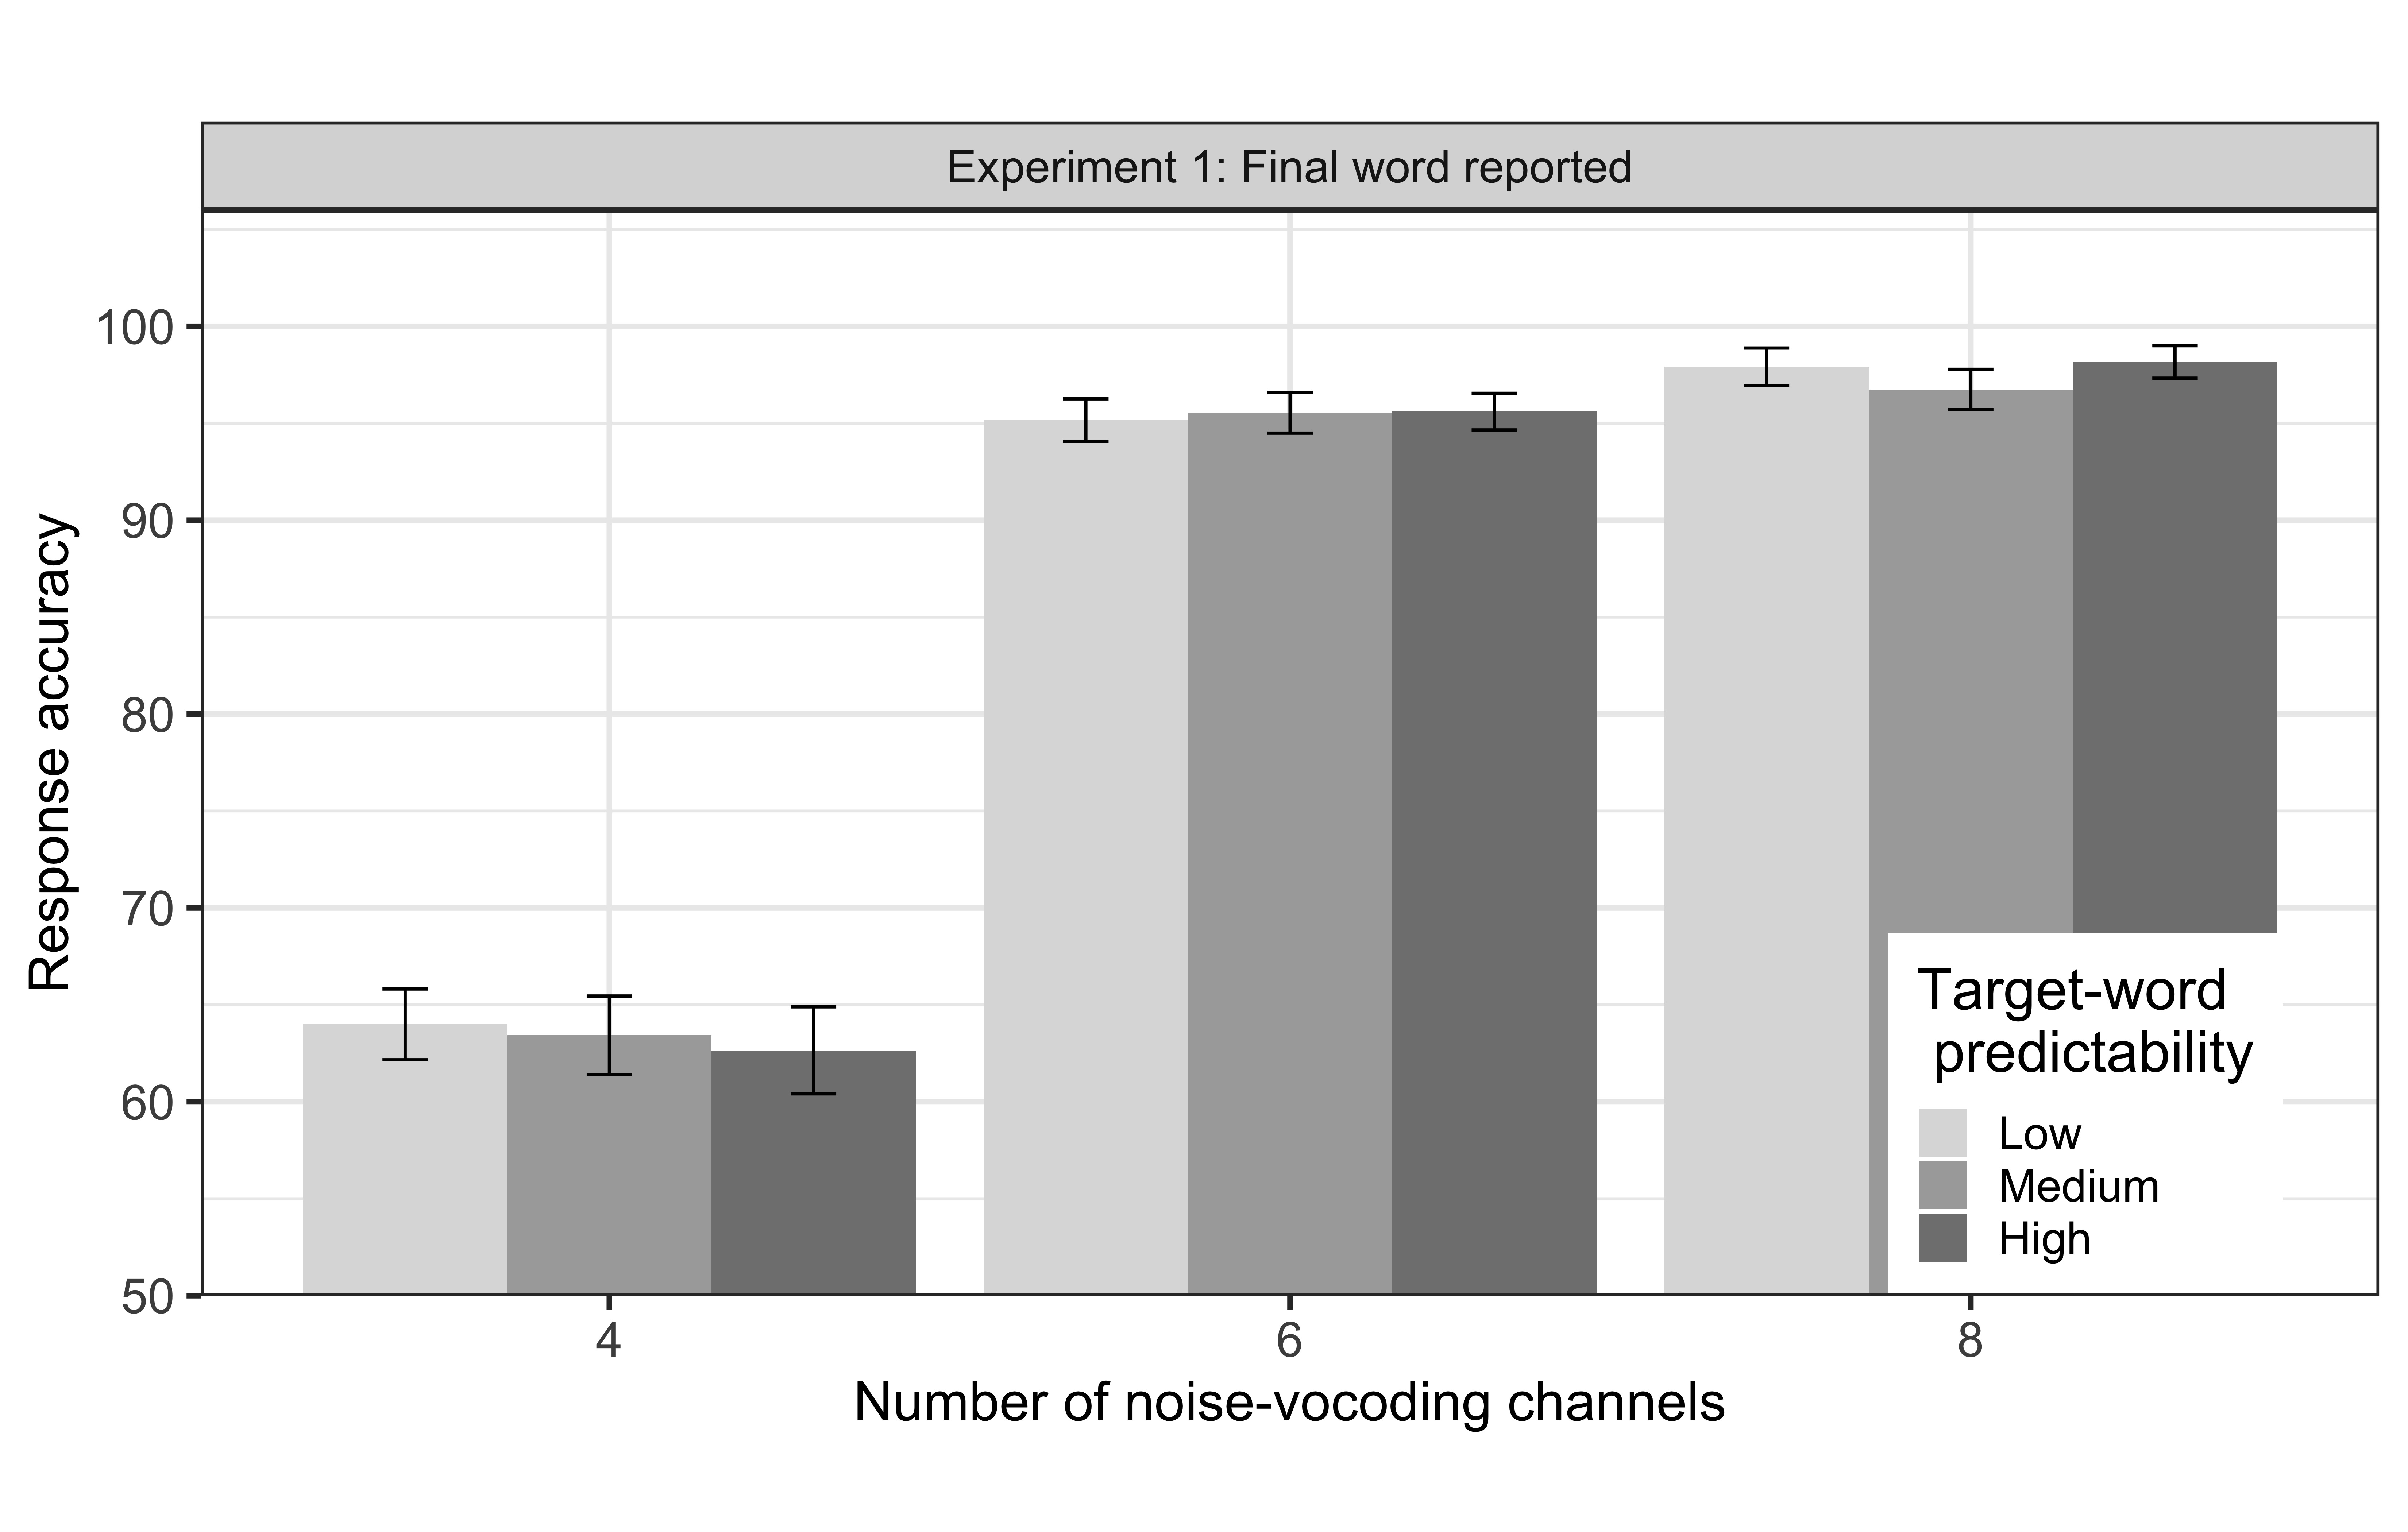
\includegraphics[width=0.95\linewidth]{figures/results-fig/expt-1a} 

}

\caption{Mean response accuracy across all conditions in Experiment 1A. Accuracy increased only with an increase in the number of noise vocoding channels. There is no change in accuracy with an increase or decrease in target word predictability. Error bars represent standard error of the means.}\label{fig:figure1a}
\end{figure}

We found that there was a significant main effect of number of channels, indicating that response accuracy in the 8 channels noise vocoded speech was higher than in both 4 channels (\(\beta\) = -3.49, SE = .23, \emph{z} (4246) = -15.30, \emph{p} \textless{} .001) and 6 channels noise vocoded speech (\(\beta\) = -.69, SE = .22, \emph{z} (4320) = -3.12, \emph{p} = .002).
That is, when the number of channels increased to 8, listeners made more correct responses.
However, there was no significant main effect of target word predictability (\(\beta\) = -.07, SE = .17, \emph{z} (4246) = -.42, \emph{p} = .68, and \(\beta\) = -.003, SE = .16, \emph{z} (4246) = -.02, \emph{p} = .98), and no significant interaction between number of noise vocoding channels and target word predictability (all \emph{p}s \textgreater{} .05).

The results of Experiment 1A indicated a decrease in response accuracy with an increase in speech degradation from 8 channels to 6 channels noise vocoding condition, and from 8 channels to 4 channels noise vocoding condition.
However, response accuracy did not increase with an increase in target word predictability,
and the interaction between number of noise vocoding channels and target word predictability was also absent, in contrast to previous findings (e.g., \protect\hyperlink{ref-Obleser2007}{Obleser et al., 2007}; \protect\hyperlink{ref-Obleser2011}{Obleser \& Kotz, 2011}; see also \protect\hyperlink{ref-Hunter2018}{Hunter \& Pisoni, 2018}).
These results suggest that the task instruction, which asked participants to only report the final word, indeed lead to neglecting the context, and therefore the facilitatory effect of prediction was not observed.
However, to further test the hypothesis --- as mentioned in the beginning of this chapter --- that predictability effect is dependent on attentional effect, we conducted another experiment.
In the second experiment, we changed the task instruction to draw participants' attention to the entire sentence such that they could attend and decode the whole sentence including the context.

\begin{longtable}[]{@{}lllll@{}}
\caption{Estimated effects of the best fitting optimal model accounting
for the correct word recognition in Experiment 1A.}
\label{results1a}
\tabularnewline
\toprule
Fixed effects & Estimate & Std. Error & \emph{z} value & \emph{p}
value \\
\midrule
\endfirsthead
\toprule
Fixed effects & Estimate & Std. Error & \emph{z} value & \emph{p}
value \\
\midrule
\endhead
Intercept & 4.20 & .24 & 17.52 & \textless.001 \\
Noise condition (4 channels) & -3.49 & .23 & -15.30 & \textless.001 \\
Noise condition (6 channels) & -.69 & .22 & -3.12 & .002 \\
Target word predictability (Low-Medium) & .07 & .17 & .42 & .67 \\
Target word predictability (High-Low) & .003 & .16 & .02 & .98 \\
\bottomrule
\end{longtable}

\hypertarget{experiment1b}{%
\section{Experiment 1B}\label{experiment1b}}

Following up on Experiment 1A, we conducted Experiment 1B on a separate group of participants with a different task instruction.
This experiment was intended to test the hypothesis that the facilitatory effect of top-down predictions is observed only when the listeners' attention is unrestricted such that the context information is also included within the attentional focus of a listener.

\hypertarget{methods-1}{%
\section{Methods}\label{methods-1}}

\hypertarget{participants-and-materials}{%
\subsection{Participants and Materials}\label{participants-and-materials}}

We recruited 48 participants (\(\bar{x}\pm SD = 24.44 \pm 3.5\) years; age range = \(18-31\) years; 32 males) online via Prolific Academic.
We used the same materials that were used in Experiment 1A.

\hypertarget{procedure-1}{%
\subsection{Procedure}\label{procedure-1}}

We followed the same procedure as in Experiment 1A with one difference:
Instead of only the final word of a sentence, participants were asked to report the entire sentence by typing in what they heard.
Guessing was encouraged.

\hypertarget{analyses-1}{%
\section{Analyses}\label{analyses-1}}

We followed the same data analyses procedure as in Experiment 1A.
The 1 channel noise vocoding condition was excluded from the analysis.
For the results of this experiment to be comparable with Experiment 1A,
we only considered the final words of the sentences (i.e., the target words) to be either correct or incorrect ---
accuracy of other preceding words were not considered in the analyses.

\hypertarget{results-and-discussion-1}{%
\section{Results and discussion}\label{results-and-discussion-1}}

Mean response accuracy for different conditions are shown in Table \ref{summary1b} and are displayed in Figure \ref{fig:figure1b}.
It shows that the accuracy increased with an increase in both the number of noise vocoding channels, and the target word predictability.

\begin{longtable}[]{@{}llll@{}}
\caption{Mean response accuracy across all levels of speech degradation
and target word predictability in Experiment 1B.}
\label{summary1b}
\tabularnewline
\toprule
Number of channels & Target word predictability & Mean & Standard
error \\
\midrule
\endfirsthead
\toprule
Number of channels & Target word predictability & Mean & Standard
error \\
\midrule
\endhead
4 & High & 62.71 & 2.14 \\
& Medium & 59.58 & 1.88 \\
& Low & 58.13 & 1.88 \\
6 & High & 96.88 & 0.93 \\
& Medium & 92.29 & 1.21 \\
& Low & 91.46 & 1.12 \\
8 & High & 98.54 & 0.86 \\
& Medium & 95.21 & 1.19 \\
& Low & 95.00 & 1.23 \\
\bottomrule
\end{longtable}

\begin{figure}

{\centering 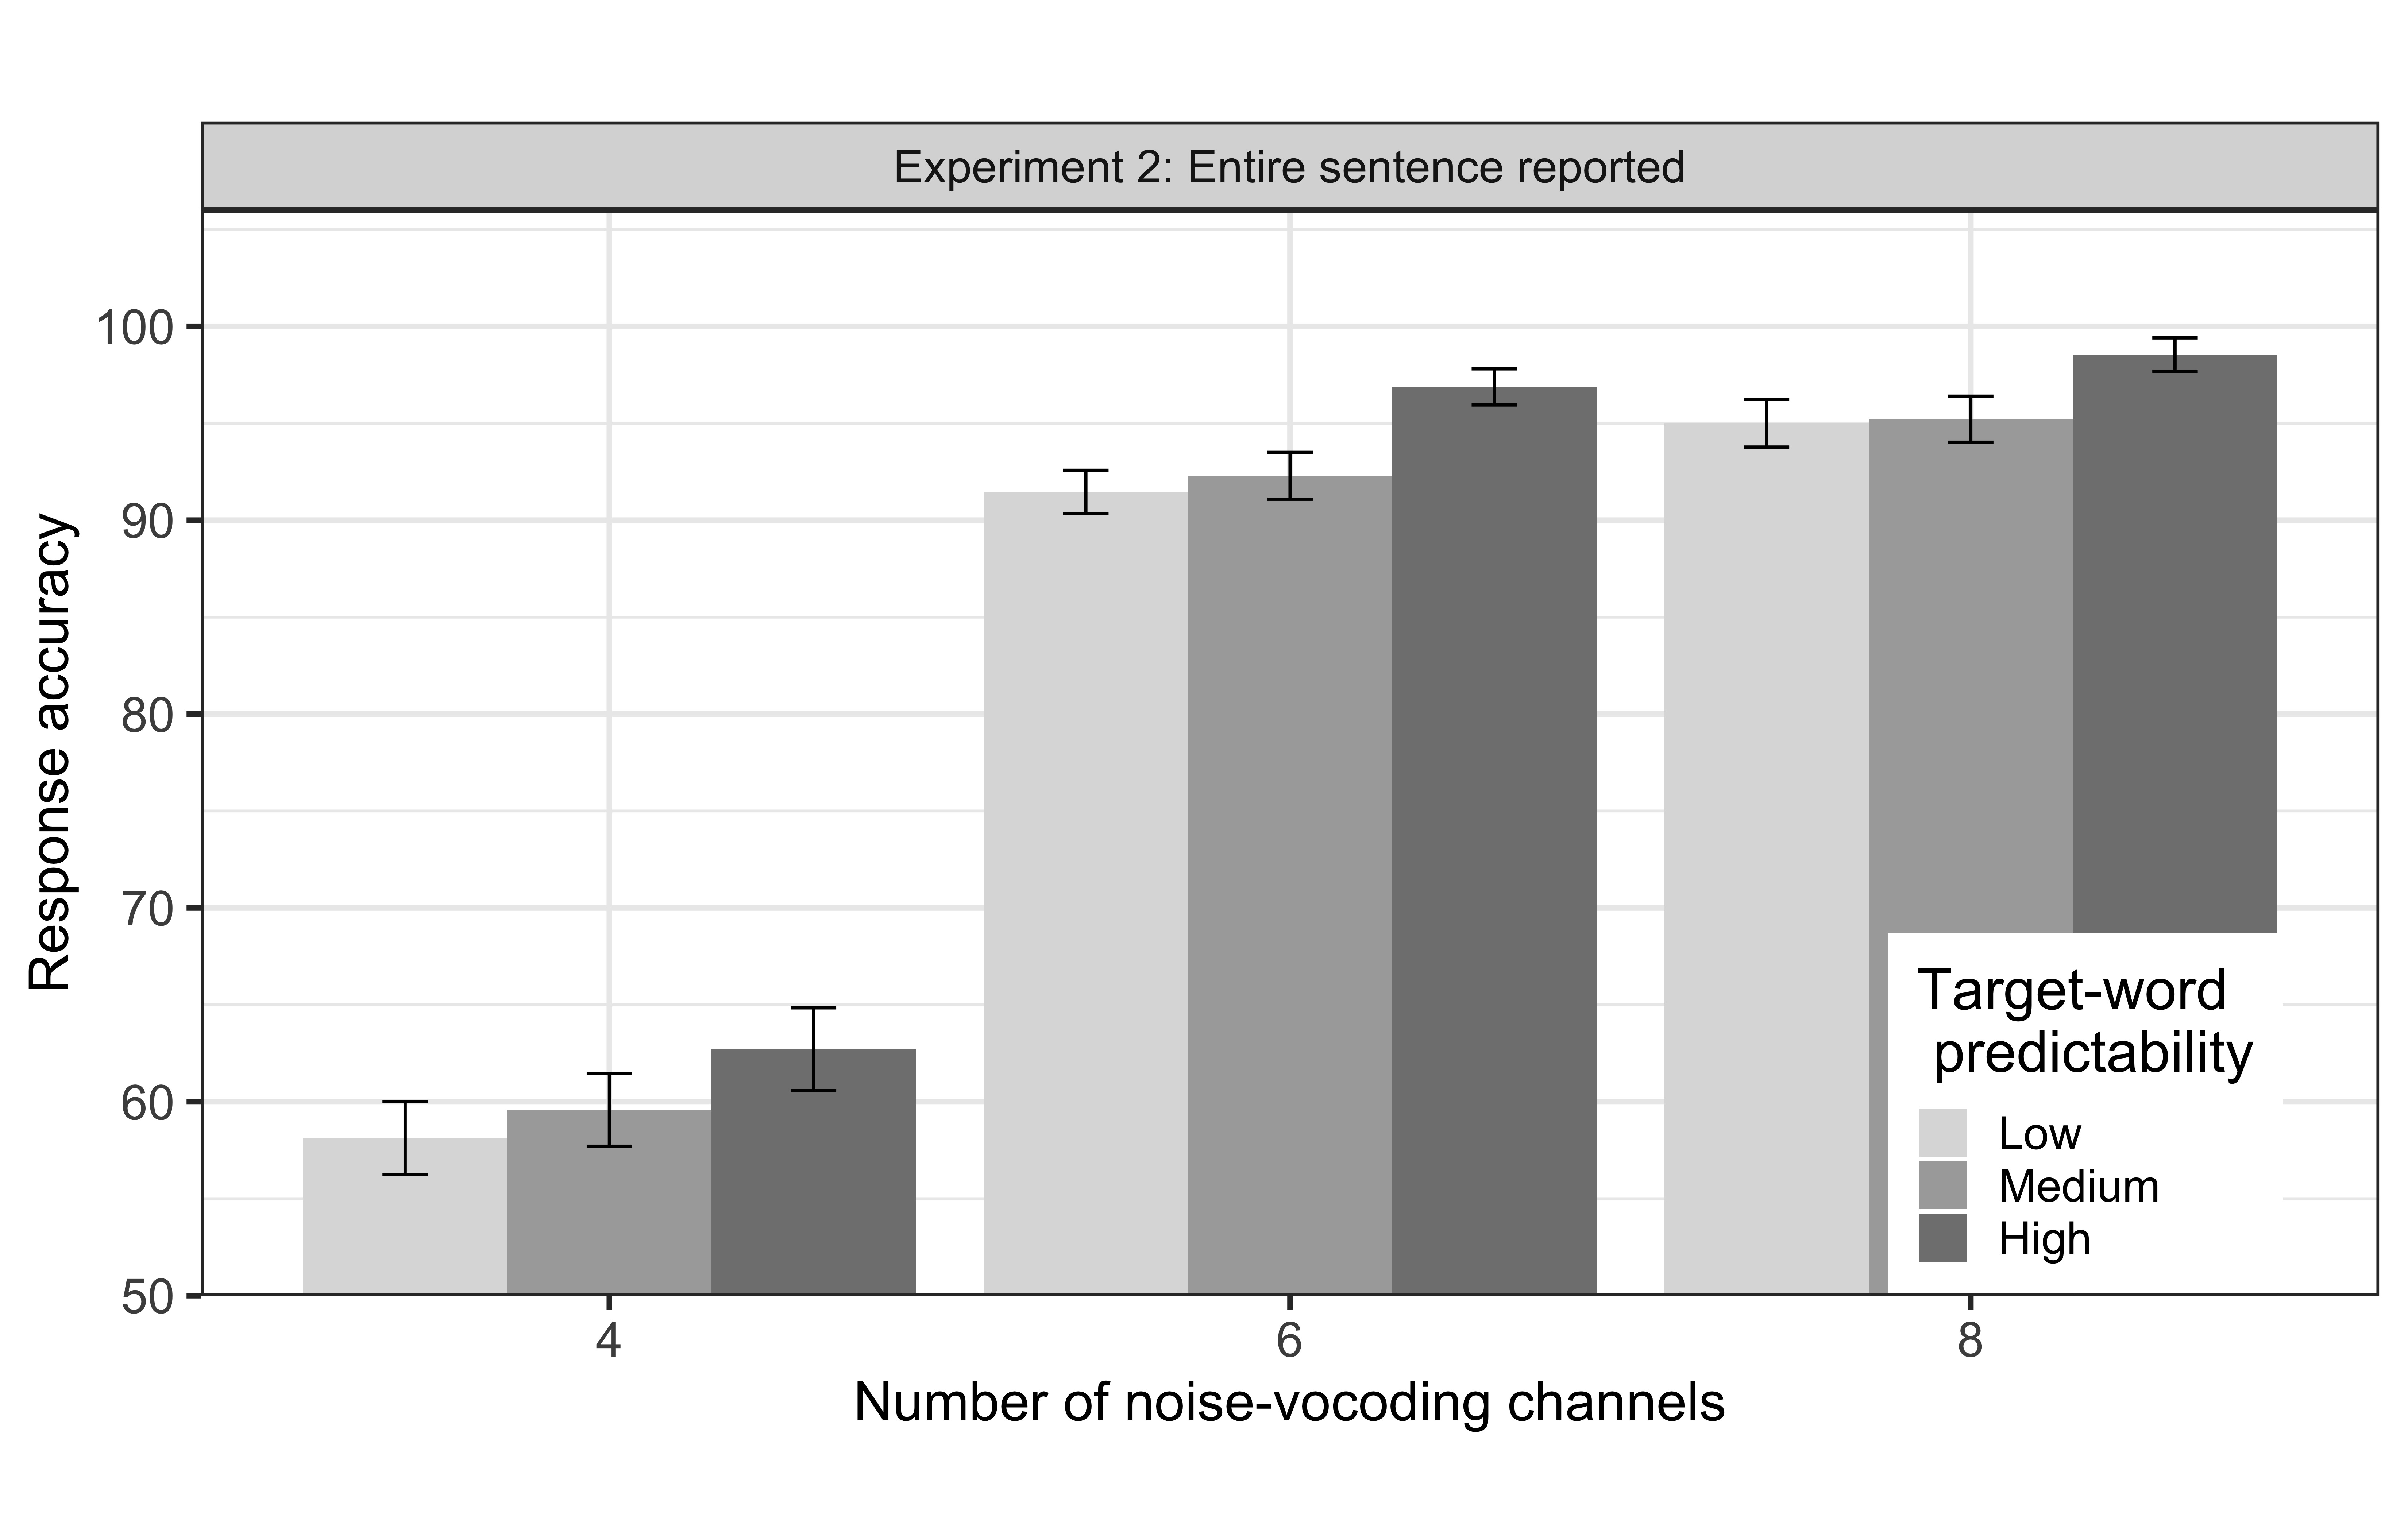
\includegraphics[width=0.95\linewidth]{figures/results-fig/expt-1b} 

}

\caption{Mean response accuracy across all conditions in Experiment 1B. Accuracy increased with an increase in number of noise vocoding channels and target word predictability. Error bars represent standard error of the means.}\label{fig:figure1b}
\end{figure}

These observations aligned with the results of the statistical analyses (Table \ref{results1b}).
We again found a main effect of number of noise vocoding channels such that response accuracy at 8 channels noise vocoding condition was higher than both 4 channels (\(\beta\) = -3.49, SE = .23, \emph{z} (4320) = -15.29, \emph{p} \textless{} .001), and 6 channels noise vocoding conditions (\(\beta\) = -0.61, SE = .20, \emph{z} (4320) = -3.07, \emph{p} = .002).
In contrast to Experiment 1A, there was also a main effect of target word predictability:
Response accuracy in high predictability sentences was significantly higher than in low predictability sentences (\(\beta\) = 1.25, SE = .28, \emph{z} (4320) = 4.50, \emph{p} \textless{} .001).
We also found a statistically significant interaction between speech degradation and target word predictability (\(\beta\) = -.95, SE = .30, \emph{z} (4320) = -3.14, \emph{p} = .002).
Subsequent subgroup analyses of each channel condition showed that the interaction was driven by the difference in response accuracy between high predictability sentences and low predictability sentences at 8 channels (\(\beta\) = 1.42, SE = .62, \emph{z} (1440) = 2.30, \emph{p} = .02), and 6 channels noise vocoding conditions (\(\beta\) = 1.14, SE = .34, \emph{z} (1440) = 3.31, \emph{p} \textless{} .001).

\begin{longtable}[]{@{}lllll@{}}
\caption{Estimated effects of the best fitting optimal model accounting
for the correct word recognition in Experiment 1B.}
\label{results1b}
\tabularnewline
\toprule
Fixed effects & Estimate & Std. Error & \emph{z} value & \emph{p}
value \\
\midrule
\endfirsthead
\toprule
Fixed effects & Estimate & Std. Error & \emph{z} value & \emph{p}
value \\
\midrule
\endhead
Intercept & 4.07 & .23 & 17.51 & \textless.001 \\
Noise condition (4 channels) & -3.49 & .23 & -15.29 & \textless.001 \\
Noise condition (6 channels) & -.61 & .20 & -3.07 & .002 \\
Target word predictability (Low-Medium) & -.10 & .16 & -.60 & .55 \\
Target word predictability (High-Low) & 1.25 & .28 & 4.50 &
\textless.001 \\
Noise condition $\times$ Target word predictability & -.95 & .30 & -3.14 &
\textless.001 \\
\bottomrule
\end{longtable}

In contrast to Experiment 1A, these results indicate an effect of target word predictability, that is, response accuracy was higher when the target word predictability was high as compared to low.
Also, the interaction between predictability and speech degradation, which was not observed in Experiment 1A, showed that semantic predictability facilitated the comprehension of degraded speech already at moderate degradation levels (like, 6 and 8 noise vocoding channels).
In line with the findings from Experiment 1A, response accuracy was better with a higher number of channels.

To test whether the difference between experimental manipulations is statistically significant, we combined the data from both the experiments in a single analysis.
We ran another binomial linear mixed-effects model on response accuracy and followed the same procedure as Experiment 1A and Experiment 1B to obtain the optimal model.
The model summary is shown in Table \ref{results1ab}.

\begin{longtable}[]{@{}lllll@{}}
\caption{Estimated effects of the best fitting optimal model accounting for the correct word recognition in both the experiments.}
\label{results1ab}
\tabularnewline
\toprule
Fixed effects & Estimate & Std. Error & \emph{z} value & \emph{p}
value \\
\midrule
\endfirsthead
\toprule
Fixed effects & Estimate & Std. Error & \emph{z} value & \emph{p}
value \\
\midrule
\endhead
Intercept & 4.09 & .23 & 17.41 & \textless.001 \\
Noise condition (4 channels) & -3.49 & .23 & -15.16 & \textless.001 \\
Noise condition (6 channels) & -.58 & .22 & -2.67 & .008 \\
Target word predictability (Low-Medium) & .15 & .27 & .57 & .57 \\
Target word predictability (High-Low) & 1.09 & .35 & 3.11 &
\textless.002 \\
Experimental group & .19 & .28 & .70 & .49 \\
Noise condition (4 channels) $\times$ Target word predictability (Low-Medium) & -.15 & .30 & -.51 &
.61 \\
Noise condition (6 channels) $\times$ Target word predictability (Low-Medium) & -.30 & .35 & -.87 &
.39 \\
Noise condition (4 channels) $\times$ Target word predictability (High-Low) & -.73 & .36 & -2.05 &
.04 \\
Noise condition (6 channels) $\times$ Target word predictability (High-Low) & -.12 & .40 & -.32 &
.75 \\
Noise condition (4 channels) $\times$ Experimental group & -.11 & .27 & -.42 &
.67 \\
Noise condition (6 channels) $\times$ Experimental group & -.11 & .30 & -.36 &
.72 \\
Target word predictability (High-Low) $\times$ Experimental group & -.45 & .18 & -2.55 &
.011 \\
\bottomrule
\end{longtable}

The model revealed that the critical interaction between experimental manipulation and target word predictability was indeed statistically significant (\(\beta\) = -.45, SE = .18, \emph{z} (8566) = -2.55, \emph{p} = .011), i.e., the effect of predictability was larger in the group that was asked to type in the whole sentence.
Together, these findings suggest that the change in task instruction, which draws attention either to the entire sentence or only to the final word, is critical for making use of the context information under degraded speech.

\hypertarget{conclusion}{%
\section{Conclusion}\label{conclusion}}

The main goals of the present study were to investigate whether online semantic predictions are formed in comprehension of degraded speech when task instructions encourage attention to the processing of the context information, or only to the critical target word.
The results of two experiments revealed that attentional processes clearly modulate the use of context information for predicting sentence endings when the speech signal is degraded.

In contrast to the first experiment, the results of the second experiment show an interaction between target word predictability and degraded speech.
This is in line with existing studies that found a facilitatory effect of predictability at different levels of speech degradation when the participants were instructed to pay attention to the entire sentence (e.g., at 4 channels or 8 channels noise vocoded speech, \protect\hyperlink{ref-Obleser2007}{Obleser et al., 2007}; \protect\hyperlink{ref-Obleser2010}{Obleser \& Kotz, 2010}).
Obleser and colleagues reported that at moderate levels of degradation, key word recognition was higher for high predictability sentences than for low predictability sentences.
Listeners were required to attend to the entire sentence in those studies as well.
Therefore, the findings of Experiment 1B replicate this facilitatory effect of predictability.

The important new finding that our study adds to the present literature is that this predictability effect may be weakened or even lost, when listeners are instructed to report only the final word of the sentence that they heard, like in Experiment 1A.
The lack of predictability effect and contextual facilitation can most likely be attributed to listeners not successfully decoding the meaning of the verb of the sentence, as the verb is the primary predictive cue for the target word (noun) in our stimuli (e.g., Sie jongliert die Baelle).
Findings from auditory attention literature also support this explanation.
When listeners' attention is focused on one feature of an auditory stimuli, the rest are not attended to and they are not processed (filter mechanism of attention, \protect\hyperlink{ref-Lange2013}{Lange, 2013})

Hence, a small change in task instruction from Experiment 1A to Experiment 1B sheds light on the role of top-down regulation of attention on using context for language comprehension in a noisy channel.
In the noisy channel when listening conditions are adverse, language comprehension is generally effortful such that focusing attention to only a part of the speech signal seems much beneficial in order to enhance stimulus decoding.
However, the results of this study also show that this comes at the cost of neglecting the context information that could be beneficial for language comprehension.
Our findings hence demonstrate that there is a trade-off between the use of context for generating top-down predictions vs.~focusing all attention on a target word.
Specifically, the engagement in the use of context and generation of top-down predictions may change as a function of attention (see also, \protect\hyperlink{ref-Li2014}{J. Li et al., 2014}).
This claim is also corroborated by the significant change in predictability effects (or contextual facilitation) from Experiment 1A to Experiment 1B, in the combined dataset.

Considering the theoretical accounts of predictive language processing (\protect\hyperlink{ref-Friston2020}{Friston, Parr, et al., 2020}; \protect\hyperlink{ref-Kuperberg2016}{Kuperberg \& Jaeger, 2016}; \protect\hyperlink{ref-Mcclelland1986}{McClelland \& Elman, 1986}; \protect\hyperlink{ref-Norris2016}{Norris et al., 2016}; \protect\hyperlink{ref-Pickering2018}{Pickering \& Gambi, 2018}), one would expect that listeners automatically form top-down predictions about upcoming linguistic stimuli based on prior context.
Also, when speech is degraded, top-down predictions render a benefit in word recognition and language comprehension (e.g., \protect\hyperlink{ref-Sheldon2008a}{Sheldon et al., 2008a}, \protect\hyperlink{ref-Sheldon2008b}{2008b}).
Results of our study revealed new theoretical insights by showing that this is not always the case.
Top-down predictions are dependent on attentional processes (see also, \protect\hyperlink{ref-Kok2012}{Kok et al., 2012}), directed by task instructions.
Thus, they are not \emph{always} automatic, and predictability does not \emph{always} facilitate language comprehension when speech is degraded.
To this point, our findings add to the growing body of literature that indicate limitations of predictive language processing accounts (\protect\hyperlink{ref-Huettig2019}{Huettig \& Guerra, 2019}; \protect\hyperlink{ref-Huettig2016}{Huettig \& Mani, 2016}; \protect\hyperlink{ref-Mishra2012}{Mishra et al., 2012}; \protect\hyperlink{ref-Nieuwland2018}{Nieuwland et al., 2018}).

In conclusion, this study provides a novel insight into the modulatory role of attention regulation in the interaction between top-down predictive and bottom-up auditory processes.
We show that task instructions affect distribution of attention to the degraded speech signal.
This, in turn, means that when insufficient attention is given to the context, top-down predictions cannot be generated, and the facilitatory effect of predictability is substantially reduced.
The findings of this study indicate limitations to predictive processing accounts of language comprehension.

\hypertarget{summary-2}{%
\section{Summary}\label{summary-2}}

This chapter replicated the previous finding that semantic predictability facilitates language comprehension at moderate levels of speech degradation.
That is, when the channel of transmission \(N\) is noisy,
listeners put less weight on the degraded auditory input \(P(u_p|u_i,N)\) and
more weight on the prior \(P(u_i,m_i)\) derived from the context information that facilitates language comprehension.
Importantly,
we found in this chapter that the contextual facilitation (i.e., facilitatory effect of predictability) is observed only when the listeners attend to the entire sentence, including the context.
In the next chapter, we further investigate this effect,
specifically, we examine the granularity of predictability effect.
We also examine if perceptual adaptation affects contextual facilitation.

\hypertarget{chapter-graded-prediction}{%
\chapter{Semantic predictability facilitates comprehension of degraded speech in a graded manner}\label{chapter-graded-prediction}}

\chaptermark{Graded effect of predictability}

In the previous chapter we concluded that in a noisy channel, predictability facilitates comprehension of degraded speech only when listeners attended to the context.
A few lacunae in the study in Chapter \ref{chapter-attention-prediction} warrant further examination and exploration of its the conclusion.
Firstly, there was an implicit assumption that all the noun-correct responses were borne out of correct identification of the context evoking words (i.e., verbs).
Instructions to the participants and the experimental design were made to test the effect of attention to context vs attention only to the target word such that
we could not test if participants identified the context correctly in \protect\hyperlink{experiment1a}{Experiment 1A}.
Secondly, we also did not consider if listeners adapted to the degraded speech, and how such an adaptation, if present, could influence contextual facilitation.
And most importantly, we only showed that there is a difference between high and low predictability sentences ---
the granularity of predictability was not tested.
Therefore, the aims of the study presented in this chapter are to address these limitations and examine if listeners form narrowed expectations or whether predictions are generated across a wide range of probable sentence endings in a graded manner.
We also take into account the accuracy of context identification (not just the accuracy of target word identification) as well as the possible learning effect due to an adaptation to the degraded speech.
The results showed that in contrast to the ``narrowed expectations'' view postulated for predictive processing of degraded speech,
listeners probabilistically preactivate upcoming words from a wide range of semantic space, not limiting only to highly probable sentence endings.
We also did not find any learning effect.
We speculate that when there is a trial-by-trial variation in semantic feature (e.g., sentence predictability), listeners do not adapt to low-level perceptual property (e.g., speech quality).

\hypertarget{introduction-1}{%
\section{Introduction}\label{introduction-1}}

In the literature of speech perception and sentence processing, studies have argued that prediction is either probabilistic and graded, or it is an all-or-nothing phenomenon (\protect\hyperlink{ref-Coltheart2004}{Coltheart, 2004}; \protect\hyperlink{ref-Kuperberg2016}{Kuperberg \& Jaeger, 2016}; \protect\hyperlink{ref-Luke2016}{Luke \& Christianson, 2016}).
Very few studies have investigated such theoretical questions within the domain of adverse listening conditions, specifically in degraded speech comprehension (e.g., \protect\hyperlink{ref-Strauss2013}{Strauß et al., 2013}; see also \protect\hyperlink{ref-Corps2020}{Corps \& Rabagliati, 2020}; \protect\hyperlink{ref-vanOs2021}{van Os et al., 2021}).
Strauß et al. (\protect\hyperlink{ref-Strauss2013}{2013}) posited that listeners cannot preactivate less predictable sentence endings in an adverse listening condition.
They proposed that the facilitatory effect of predictability is limited to only highly predictable sentence endings at a moderate level of spectral degradation of speech.
Although many studies support the general idea of Strau\ss~and colleagues that predictability facilitates comprehension of degraded speech (e.g., \protect\hyperlink{ref-Hunter2018}{Hunter \& Pisoni, 2018}; \protect\hyperlink{ref-Obleser2010}{Obleser \& Kotz, 2010}; \protect\hyperlink{ref-Sheldon2008a}{Sheldon et al., 2008a}),
there have been no studies so far after Strau\ss~and colleagues', to our knowledge, which examined the nature of predictability specifically in degraded speech comprehension.

In this chapter, our main aim is to replicate the previous findings of these predictability effects,
and extend them further by testing if listeners form narrowed expectations while listening to moderately degraded speech.
In line with Strauß et al. (\protect\hyperlink{ref-Strauss2013}{2013})'s argument, listeners can form predictions that are restricted to only highly probable sentence endings.
On the opposite, listeners can generate expectations about an upcoming word based on how likely the word is to appear in the context,
and hence form a probabilistic prediction.
We also test the presence of perceptual adaptation and its effect on contextual facilitation.
We set a metric of measurement of language comprehension that considers whether listeners correctly identified the context information.

\hypertarget{background-1}{%
\section{Background}\label{background-1}}

\hypertarget{predictability-effects-in-degraded-speech-perception}{%
\subsubsection{Predictability effects in degraded speech perception}\label{predictability-effects-in-degraded-speech-perception}}

\noindent
We discussed in Chapter \ref{chapter-background} (Section \ref{background-facilitatory-effect})
that some studies (\protect\hyperlink{ref-Obleser2007}{Obleser et al., 2007}; \protect\hyperlink{ref-Obleser2010}{Obleser \& Kotz, 2010}; \protect\hyperlink{ref-Sheldon2008a}{Sheldon et al., 2008a}; see also, \protect\hyperlink{ref-Hunter2018}{Hunter \& Pisoni, 2018}) have already shown the facilitatory effect of predictability in comprehension of degraded speech.
For example, Obleser and colleagues compared high and low predictability sentences and observed contextual facilitation, in terms of the difference in response accuracy between high and low predictability sentences, at 8 channels and 4 channels noise vocoded speech in their (\protect\hyperlink{ref-Obleser2007}{2007}) and (\protect\hyperlink{ref-Obleser2010}{2010}) studies respectively.
However, these neuroimaging studies were not designed to test the nature of predictability effects.

In a modified experimental design, Strauß et al. (\protect\hyperlink{ref-Strauss2013}{2013}) varied the target word predictability by manipulating its expectancy (i.e., how expected the target word is given the verb) and typicality (i.e., co-occurrence of target word and the preceding verb).
They reported that at a moderate level of spectral degradation, N400 responses at highly predictable (strong-context and high-typical) words were smallest.
In contrast, they found that the N400 effect (in terms of the amplitude of the N400 component) were largest at the strong-context, low typical words and the weak-context, low-typical words;
the responses at the latter two were not statistically different from each other.
The authors interpreted these findings as a facilitatory effect of sentence predictability which might be limited to only highly predictable sentence endings at a moderate level of spectral degradation.
They proposed it as an \emph{expectancy searchlight model}, and suggested that listeners form \emph{narrowed expectations} from a restricted semantic space when the sentence endings are highly predictable.
Their model posits that when the sentence endings are less predictable, listeners cannot preactivate those less predictable sentence endings in an adverse listening condition.
This is contrary to the view that readers and listeners form a probabilistic prediction of upcoming word in a sentence.
For example, Nieuwland et al. (\protect\hyperlink{ref-Nieuwland2018}{2018})\footnote{However, Nieuwland et al.~(2018) could not replicate DeLong et al.~(2005)'s finding that comprehenders predict word-form -- English articles \emph{a/an}.} showed in a large-scale replication study of DeLong et al. (\protect\hyperlink{ref-Delong2005}{2005}) that the N400 amplitude at the sentence-final noun is directly proportional to its cloze probability across a range of high- and low-cloze words (see also, \protect\hyperlink{ref-Kochari2019}{Kochari \& Flecken, 2019}; \protect\hyperlink{ref-Nicenboim2020}{Nicenboim et al., 2020}).
Heilbron et al. (\protect\hyperlink{ref-Heilbron2021}{2021}) also showed that a probabilistic prediction model outperforms a constrained guessing model in predicting listeners' neural activities (MEG and EEG recordings),
suggesting that linguistic prediction is probabilistic and it is not limited only to the highly predictable sentence endings, but it operates broadly in a wide range of probable sentence endings.
However, when put in perspective with our research question, these studies were conducted in conditions without noise or degraded speech.
And those studies that examined degraded speech comprehension, used only two levels of semantic predictability (high and low).
The granularity and the nature of prediction remain yet to be tested in degraded speech comprehension.

\hypertarget{adaptation-to-degraded-speech}{%
\subsubsection{Adaptation to degraded speech}\label{adaptation-to-degraded-speech}}

\noindent
We discussed in Chpater \ref{chapter-background} that studies have shown evidence for perceptual adaptation to artificially distorted speech.
When exposed to noise vocoded speech, listeners' word recognition accuracy increased over the course of experiment (\protect\hyperlink{ref-Davis2005}{Davis et al., 2005}; \protect\hyperlink{ref-Erb2013}{Erb et al., 2013})
These studies have only used one noise-vocoded speech (e.g., 4 channels, or 6 channels) as stimuli, and presented such degraded speech in a single block.
From a participant's (listener's) perspective, there was no uncertainty about the degradation level of next trial speech, i.e., the \emph{global channel context} was certain or predictable.
Additionally, there was no variation in semantic feature, especially, target word predictability.

Listeners gradually map the representation of degraded lexicons around their ``true'' (or clear) schema/exemplars on repeated exposure (\protect\hyperlink{ref-Goldstone1998}{Goldstone, 1998}; \protect\hyperlink{ref-Nosofsky1986}{Nosofsky, 1986}).
With repeated exposure, the representation of degraded input comes closer to the exemplar, thereby, improving the performance.
This feature mapping mechanism proposes that listeners map the whole feature of the sensory input.
However, the higher level features of speech (e.g., semantic property like predictability) can also influence the acoustic realization of a degraded word,
i.e., bottom-up processing of the degraded speech and perceptual adaptation (\protect\hyperlink{ref-Gold2010}{Gold \& Watanabe, 2010}; \protect\hyperlink{ref-Goldstone1998}{Goldstone, 1998}).
Listeners can assign weight to different dimensions of a speech stimuli (acoustic-phonetic and/or lexico-semantic).
Performance improves over time when listeners give more attentional weight to acoustic-phonetic dimension (cf. \protect\hyperlink{ref-Haider1996}{Haider \& Frensch, 1996}).

Thus, when multiple levels of degraded speech signals are presented in a block in a (pseudo-)randomized order, then the listener is uncertain about the quality of next-trial's speech.
If such multiple levels of degradation are due to the presentation of multiple channels of noise vocoded speech, then the global channel context is unpredictable or uncertain.
This can render perceptual adaptation totally absent with the change in the auditory features of the speech signal throughout the experiment (\protect\hyperlink{ref-Mattys2012}{Mattys et al., 2012}).
Additionally, such trial-by-trial variability in the characteristics of speech signal can also impair word recognition (\protect\hyperlink{ref-Sommers1994}{Sommers et al., 1994}; see also, \protect\hyperlink{ref-Dahan2006}{Dahan \& Magnuson, 2006}).
Very few studies have examined the influence of (un)certaintly about nex-trial speech quality, and semantic feature in perceptual adaptation.
For example, Vaden et al. (\protect\hyperlink{ref-Vaden2013}{2013}) presented participants words in background noise at +3dB SNR and +10dB SNR, instead of a degraded speech, in a pseudo-random order.
They argued that an adaptive control system is involved to optimize task performance when there is an uncertainty about next trial.
Obleser and colleagues (\protect\hyperlink{ref-Hartwigsen2015}{Hartwigsen et al., 2015}; \protect\hyperlink{ref-Obleser2007}{Obleser et al., 2007}; \protect\hyperlink{ref-Obleser2010}{Obleser \& Kotz, 2010}) presented listeners with multiple noise-vocoded speech (ranging from 2 to 32 channels noise vocoding) in a pseudo-random order, but they did not report presence or absence of perceptual adaptation.
As previously mentioned in Chapter \ref{chapter-background} (Section \ref{background-adaptation}), there are two conflicting findings in the literature on perceptual adaptation:
On the one hand, repeated exposure to degraded speech leads to perceptual adaptation, and consequently improves word recognition over the course of experiment.
On the other hand, uncertainty about next-trial speech quality impairs word recognition.

\hypertarget{chapter-6-measurement}{%
\subsubsection{Measurement of language comprehension}\label{chapter-6-measurement}}

\noindent
How we measure language comprehension has rarely been guided by any specific theoretical motive in the existing literature.
There is a discrepancy across studies in how language comprehension in degraded speech in quantified.
Some studies that reported contextual facilitation in degraded speech comprehension used proportion of correctly reported \emph{final} words only (e.g., \protect\hyperlink{ref-Hunter2018}{Hunter \& Pisoni, 2018}; \protect\hyperlink{ref-Obleser2010}{Obleser \& Kotz, 2010}; \protect\hyperlink{ref-Sheldon2008a}{Sheldon et al., 2008a}).
Obleser et al. (\protect\hyperlink{ref-Obleser2007}{2007}) quantified language comprehension as the proportion of correctly identified key words in SPIN sentences.
Erb et al. (\protect\hyperlink{ref-Erb2013}{2013}) and Hakonen et al. (\protect\hyperlink{ref-Hakonen2017}{2017}) used \emph{report scores} (\protect\hyperlink{ref-Peelle2013}{Peelle, 2013}) that measure proportion of correctly recognized words per sentence as an index of language comprehension.
Such inconsistencies make cross-study comparison difficult.
Additionally, none of these measures take into account if listeners have correctly identified the context (cf. \protect\hyperlink{ref-Amichetti2018}{Amichetti et al., 2018}; \protect\hyperlink{ref-Marrufo2019}{Marrufo-Pérez et al., 2019})
which should be the most important factor to be considered in the first place.

\hypertarget{the-present-study}{%
\subsubsection{The present study}\label{the-present-study}}

\noindent
Stemming from the results of Chapter \ref{chapter-attention-prediction}, and from the motivation driven by the open questions outlined in the beginning of this chapter, the goals of the study in this chapter were threefold:
The first goal was to replicate the facilitatory effect of predictability, and examine the nature of predictability, i.e., to test if listeners form narrowed expectations.
Obleser and colleagues (e.g., \protect\hyperlink{ref-Obleser2007}{Obleser et al., 2007}; \protect\hyperlink{ref-Obleser2010}{Obleser \& Kotz, 2010}) have shown predictability effects (or contextual facilitation) to appear only at a moderate level of speech degradation by using only two levels of predictability (low and high).
Our use of three levels of target word predictability (low, medium and high) will let us test the narrowed expectations view (\protect\hyperlink{ref-Strauss2013}{Strauß et al., 2013}) by also taking into account the accuracy of context.
If the listeners form narrowed predictions only for the target words with high cloze probability, then the facilitatory effect of semantic prediction will be observed only at these highly predictable sentence endings.
Listeners' response to the target words with medium and low cloze probability would be quite similar as these two fall out of the range of narrow prediction.
However, if the listeners' predictions are not restricted to highly predictable target words, then they form predictions across a wide range of context proportional to the probability of occurrence of the target word.
In addition to highly predictable sentence endings, listeners will also form predictions for less predictable sentence endings.
Such predictions will depend on the probability of occurrence of the target words.
In other words, listeners form predictions also for less expected sentence endings;
and the semantic space of prediction depends on the probability of occurrence of those sentence endings.
The addition of sentences with medium cloze target words thus allows us to differentiate whether listeners form all-or-nothing prediction restricted to high cloze target words, or a probabilistic prediction for words across a wide range of cloze probability.

There is a variation in the sentences we use, i.e., they are low, medium and high predictability sentences, and they are degraded at different levels of spectral degradation.
So our second goal was to investigate the role of uncertainty about next-trial speech features on perceptual adaptation by varying the global channel context on the comprehension of degraded speech.
To study this, we presented sentences of different levels of predictability blocked by each channel conditions (\emph{predictable channel context}), and pseudo-randomized across all channels (\emph{unpredictable channel context}).
Based on previous findings, we expected that in the unpredictable channel context (i.e., when sentences are presented in a random order of spectral degradation) participants' word recognition performance will be worse than in the predictable channel context (i.e., when the sentences are blocked by noise-vocoding, \protect\hyperlink{ref-Garrido2011}{Garrido et al., 2011}; \protect\hyperlink{ref-Sommers1994}{Sommers et al., 1994}; \protect\hyperlink{ref-Vaden2013}{Vaden et al., 2013}).
To further examine perceptual adaptation, we also considered the effect of trial number in the analyses.

And third, we aimed at measuring language comprehension with a metric that reflects the participants' correct or incorrect identification of the context.
If participants do not understand the context and we only measure the recognition of final word, this might not truly reflect the effect of contextual facilitation.

\hypertarget{methods-2}{%
\section{Methods}\label{methods-2}}

\hypertarget{participants-1}{%
\subsection{Participants}\label{participants-1}}

We recruited a group of participant via Prolific Academic and assigned them to the \emph{predictable channel context} (n = 50; \(\pm\) SD = 23.6 \(\pm\) 3.2 years; age range = 18 -- 30 years; 14 females).
We created \emph{unpredictable channel context} group from participants (n = 48; \(\bar{x}\) \(\pm\) SD = 24.44 \(\pm\) 3.5 years; age range = 18 -- 31 years; 16 females) from \protect\hyperlink{experiment1b}{Experiment 1B}.
All participants were native speakers of German residing in Germany.
We recruited onlty those participants who had reported to not have any hearing disorder, speech-language disorder, or neurological disorder.

\hypertarget{materials-1}{%
\subsection{Materials}\label{materials-1}}

We used the same stimuli described in Chapter \ref{chapter-methods} (Section \ref{experimental-materials}).
We used 120 sentences each for low predictability, medium predictability, and high predictability sentences that differed in the cloze probability of sentence final target words.
Their mean cloze probabilities were \(0.022\pm0.027\) (\(\bar{x}\pm SD\); range = \(0.00-0.09\)) for low predictability sentences, \(0.274\pm0.134\) (\(\bar{x}\pm SD\); range = \(0.1-0.55\)) for medium predictability sentences, and \(0.752\pm0.123\) (\(\bar{x}\pm SD\); range = \(0.56-1.00\)) for high predictability sentences.

In the unpredictable channel context, each participant was presented with 120 unique sentences: 40 low predictability, 40 medium predictability, and 40 high predictability sentences.
Channel condition (i.e., degradation level) was also balanced across each sentence type, i.e., in each of low, medium, and high predictability sentences, 10 sentences passed through each noise vocoding channels --- 1, 4, 6, and 8 --- were presented.
This resulted into 12 experimental lists.
The sentences in each list were pseudo-randomized, that is, not more than three sentences of same noise condition (i.e., same noise vocoding channel), or same predictability condition appeared consecutively.
This randomization confirmed the uncertainty of next-trial speech quality (or degradation) in the global context of the experiment.

The same set of stimuli and experimental lists were used in the predictable channel context.
Each participant was presented with 120 unique sentences blocked by channel conditions, i.e., blocked by noise vocoding channels.
There were four blocks of stimuli, one for each channel condition (i.e., degradation level).
Thirty sentences were presented in each of the four blocks.
In the first block, all sentences were 8 channels noise vocoded, followed by the blocks of 6 channels, 4 channels, and 1 channel noise vocoded speech consecutively (\protect\hyperlink{ref-Sheldon2008a}{Sheldon et al., 2008a}).
Within each block, 10 low predictability, 10 medium predictability and 10 high predictability sentences were presented.
All the sentences were pseudo-randomized so that not more than three sentences of the same predictability condition appeared consecutively in each block.
This confirmed there was a certainty of next-trial speech quality (within each block) and an uncertainty of next-trial sentence predictability across all four blocks.

\hypertarget{procedure-2}{%
\subsection{Procedure}\label{procedure-2}}

Participants were asked to use earphones or headphones.
A prompt to adjust loudness was displayed at the beginning of the experiment:
A noise vocoded sound not used in the main experiment was presented, and participants were asked to adjust the loudness at their level of comfort.
One spoken sentence was presented in each trial with an inter-trial interval of 1000ms.
Eight practice trials were presented before presenting 120 experimental trials.
They were asked to enter what they had heard (i.e., to type in the entire sentence).
Guessing was encouraged.
The response was not timed.
The experiment was about 40 minutes long.

\hypertarget{analyses-2}{%
\section{Analyses}\label{analyses-2}}

In the sentences used in our experiment, verbs evoke predictability of the sentence-final noun.
Therefore, the effect of predictability (evoked by the verb) on language comprehension can be rightfully measured if we consider only those trials in which participants identify the verbs correctly.
Verb-correct trials were considered as the sentence in which participants identified the context independent of whether they correctly understood the sentence final target noun.
Morphological inflections and typos were considered as correct.
We first filtered out those trials in which verbs were not identified correctly, i.e., trials with incorrect verbs.
Therefore, we excluded 2469 out of 5760 trials in unpredictable channel context and 2374 out of 6000 trials in predictable channel context from the analyses.
The 1 channel noise vocoding condition was dropped from the analyses as there were no correct responses in any of the trials in this condition.

We analyzed response accuracy with generalized linear mixed models following the procedure described in Chapter \ref{chapter-stats} (Section \ref{analysis-main}).
Binary responses (correct/incorrect) for all participants in both groups (predictable channel context and unpredictable channel context) were fit with a binomial logistic mixed-effects model (\protect\hyperlink{ref-Jaeger2006}{Jaeger, 2006}, \protect\hyperlink{ref-Jaeger2008}{2008}).
Noise condition (categorical; 4, 6, and 8 channels noise vocoding), target word predictability (categorical; high predictability, medium predictability, and low predictability), global channel context (categorical; predictable channel context and unpredictable channel context), and the interaction of noise condition and target word predictability were included in the fixed effects.
We applied treatment contrast for noise condition (8 channels as a baseline; factor levels: 8 channels, 4 channels, 6 channels) and sliding difference contrast for target word predictability (factor levels: medium predictability, low predictability, high predictability) and channel context (factor levels: unpredictable, predictable).

\hypertarget{results-and-discussion-2}{%
\section{Results and discussion}\label{results-and-discussion-2}}

We observed that the mean response accuracy increased with an increase in number of noise vocoding channels from 4 to 6 to 8, and with an increase in target word predictability from low to medium to high (see Figure X.X).
This trend was consistent across both the channel contexts;
Figure X.X and Figure Y.Y show this trend for predictable channel context (i.e., blocked design) and unpredictable channel context (i.e., randomized design) respectively.
Mean accuracies across all conditions are given in Table X and Y, and Figure X.X.

These observations are confirmed by the results of statistical analyses (Table XYZ).
We found a significant main effect of channel condition indicating that the response accuracy was higher in the 8 channels
than in the 4 channels (\(\beta\) = -2.87, SE = .22, \emph{z} (6917) = -13.1, \emph{p} \textless.001) and
6 channels (\(\beta\) = -.66, SE = .19, \emph{z} (6917) = -3.42, \emph{p} \textless{} .001).
There was a significant main effect of target word predictability suggesting that response accuracy was lower at low predictability sentences
than both high predictability sentences (\(\beta\) = 2.18, SE = .3, \emph{z} (6917) = 7.2, \emph{p} \textless{} .001) and
medium predictability sentences (\(\beta\) = -.52, SE = .27, \emph{z} (6917) = -1.97, \emph{p} = .049).
We also found a significant interaction between channel condition and target word predictability (\(\beta\) = -.71, SE = .29, \emph{z} (6917) = -2.44, \emph{p} = .015).

We performed a subgroup analyses on each noise channel condition
which revealed that the interaction was driven by the effect of predictability at 4 channels:
The accuracy at high predictability sentences was higher than medium predictability sentences (\(\beta\) = 1.14, SE = .37, \emph{z} (1608) = 3.1, \emph{p} \textless{} .001),
which in turn was also higher than low predictability sentences (\(\beta\) = 1, SE = .24, \emph{z} (1608) = 4.2, \emph{p} \textless{} .001).
There was no significant difference in response accuracy between low predictability and high predictability sentences
at both 6 channels (\(\beta\) = .33, SE = .32, \emph{z} (2590) = 1.04, \emph{p} = .3)
and 8 channels (\(\beta\) = -.014, SE = .32, \emph{z} (2719) = -.04, \emph{p} = .97).

We also found a significant main effect of global channel context which showed that the response accuracy was higher in predictable channel context than in unpredictable channel context (\(\beta\) = -.27, SE = .14, \emph{z} (6917) = -2.02, \emph{p} = .04).

Further, to test the effect of practice on adaptation to degraded speech, we added trial number as a fixed effect in the maximal model.
Note that there were 30 trials in each block in the predictable channel context (i.e., blocked design).
For comparability, we divided unpredictable channel context (i.e., randomized design) into four blocks in the analysis.
We did not find a significant main effect of trial number indicating that the response accuracy did not change throughout the experiment (\(\beta\) = -.0004, SE = .01, \emph{z} (6917) = -.05, \emph{p} = .97).
It remained constant within each block in the predictable channel context (\(\beta\) = -.02, SE = .01, \emph{z} (3291) = -1.43, \emph{p} = .15) as well as in the unpredictable channel context (\(\beta\) = .01 SE = .01, \emph{z} (3291) = 1.05, \emph{p} = .29).

\hypertarget{conclusion-1}{%
\section{Conclusion}\label{conclusion-1}}

The present study had three goals: i) to examine if previously reported facilitatory effect of semantic predictability is restricted to only highly predictable sentence endings;
ii) to assess the role of perceptual adaptation on the facilitation of language comprehension by sentence predictability; and
iii) to use and establish a sensitive metric to measure language comprehension that takes into account whether listeners benefited from the semantic context of the sentence they have listened to.

Results of our study showed the expected interaction between predictability and degraded speech, that is, language comprehension was better for high-cloze than for low-cloze target words when the speech signal was moderately degraded by noise vocoding through 4 channels, while the effect of predictability was absent when speech was not intelligible (noise vocoding through 1 channel).
These results are fully in line with Obleser \& Kotz (\protect\hyperlink{ref-Obleser2010}{2010});
we partly included identical sentences from their study in the present study (see Appendix A).
Importantly, in contrast to their study, we had also created sentences with medium-cloze target words (which were intermediate between high-cloze and low-cloze target words) and found that the effect of predictability was also significant when comparing sentences with medium-cloze target words against sentences with low-cloze target words at 4 channels noise vocoding condition.
Recognition of a target word was dependent on its level of predictability (measured by cloze probability), and correct recognition was not just limited to high-cloze target words.
These significant differences in response accuracy between medium-cloze and low-cloze target words, and between medium-cloze and high-cloze target words at noise-vocoding through 4 channels show that the sentence-final word recognition is facilitated by semantic predictability in a graded manner.
This is in line with the findings from the ERP literature where it has been observed that semantic predictability, in terms of cloze probability of target word of a sentence, modulates semantic processing, indexed by N400, in a graded manner (\protect\hyperlink{ref-Delong2005}{DeLong et al., 2005}; \protect\hyperlink{ref-Nieuwland2018}{Nieuwland et al., 2018}; \protect\hyperlink{ref-Wlotko2012}{Wlotko \& Federmeier, 2012}).

The interpretation of the observed graded effect of semantic predictability at the moderate level of spectral degradation (i.e., at noise-vocoding through 4 channels) provides a novel insight into how listeners form prediction when the bottom-up input is compromised.
That is, in an adverse listening condition, listeners rely more on top-down semantic prediction than on bottom-up acoustic-phonetic cues.
However, such a reliance on top-down prediction is not an all-or-nothing phenomenon; instead, listeners form a probabilistic prediction of the target word.
The effect of target word predictability on comprehension is not sharply focused solely on high-cloze target words like a `searchlight' as proposed by Strau\ss~and colleagues.
But rather it is spread across a wide range including low-cloze and medium-cloze target words.
As the cloze probability of the target words decreases from high to low, the focus of the searchlight becomes less precise.

We did not find learning effects at the trial-by-trial level of perceptual adaption: it may be that the adaptation was hampered by variation in higher-level semantic features (i.e., target word predictability).
We also argue that for the examination of semantic predictability effects during language comprehension, the analyses of response accuracy should be based on the trials in which context evoking words are correctly identified in the first place to make sure that listeners make use of the contextual cues instead of analyzing general word recognition scores.

\hypertarget{summary-3}{%
\section{Summary}\label{summary-3}}

This chapter investigated the nature of predictability effect that was tested earlier in Chapter \ref{chapter-attention-prediction}.
The studies provide a novel insight into predictive language processing when bottom-up signal quality is compromised and uncertain:
We show that while processing moderately degraded speech, listeners form top-down predictions across a wide range of semantic space that is not restricted within highly predictable sentence endings.
In contrast to the \emph{narrowed expectations} view, comprehension of words ranging from low- to high-cloze probability, including the medium-cloze probability, is facilitated in a graded manner while listening to a moderately degraded speech.
Regardless of (un)certainty about the next-trial speech quality, we find that listeners do not adapt to degraded speech when semantic predictability varies,
i.e., higher level semantic features interfere with the lower level perceptual properties.
In the next chapter,
we investigate the effect of changes in the lower-level bottom-up processing on top-down semantic predictions.
Specifically, we examine how the change in speech rate moderates semantic predictions at a moderate level of speech degradation.

\hypertarget{chapter-speech-rate}{%
\chapter{Comprehension of degraded speech is modulated by the rate of speech}\label{chapter-speech-rate}}

\chaptermark{Speech rate and predictability effects}

\hypertarget{introduction-2}{%
\section{Introduction}\label{introduction-2}}

\hypertarget{background-2}{%
\section{Background}\label{background-2}}

Language comprehension depends on the features and quality of speech signal
which is hampered in adverse listening conditions when speech is distorted, for example, due to change in rate of speech, and spectral degradation of speech.
Studies have shown that individuals can benefit from sentence context to compensate for distorted speech, at least when the level of speech degradation is at an intermediate level (\protect\hyperlink{ref-Bhandari2021}{Bhandari et al., 2021}; e.g., \protect\hyperlink{ref-Obleser2010}{Obleser \& Kotz, 2010}), and at varying speech rate (\protect\hyperlink{ref-Aydelott2004}{Aydelott \& Bates, 2004}; cf. \protect\hyperlink{ref-Goy2013}{Goy et al., 2013}).
The goal of the present study is to examine if sentence context can provide benefit when speech that is degraded at an intermediate level is presented at different rates (from slow, normal, and fast); speech in day-to-day conversation is distorted and presents itself at varying rate (e.g., \protect\hyperlink{ref-Krause2004}{Krause \& Braida, 2004}).
In the following, we first summarize the impact of speech degradation in language comprehension, and its interaction with sentence context, and then the influence of speech rate on language comprehension, and its interaction with sentence context.

\hypertarget{comprehension-of-degraded-speech}{%
\subsection{Comprehension of degraded speech}\label{comprehension-of-degraded-speech}}

There are a number of studies showing that speech intelligibility and language comprehension is hampered when the bottom-up input is less intelligible due to spectral degradation of the speech signal (\protect\hyperlink{ref-Davis2005}{Davis et al., 2005}; \protect\hyperlink{ref-Shannon1995}{Shannon et al., 1995}).
These studies have used noise vocoding as a methods of speech degradation. Here the speech signal is first divided into a specific number of frequency bands that corresponds to the number of vocoder channels.
The amplitude envelope within each frequency band is extracted, and the spectral information within it is replaced by noise.
The resulting vocoded speech contains temporal cues of the original speech, but it is difficult to understand -- the lesser the number of vocoder channels, the lesser is the intelligibility.
More attentional resources are required to process and comprehend such degraded speech as compared to clean speech (\protect\hyperlink{ref-Eckert2016}{Eckert et al., 2016}; e.g., \protect\hyperlink{ref-Wild2012}{Wild et al., 2012}).

Listeners rely more on top-down predictions when the speech signal is less intelligible due to spectral degradation.
Hence, they use the context information of the sentence to narrow down their predictions to a smaller set of semantic categories or words (\protect\hyperlink{ref-Strauss2013}{Strauß et al., 2013}; see also, \protect\hyperlink{ref-Corps2020}{Corps \& Rabagliati, 2020}).
However, it is important that the context itself is `intelligible enough' which is the case when the speech is only moderately degraded.
For example, Obleser and colleagues (\protect\hyperlink{ref-Obleser2007}{Obleser et al., 2007}; \protect\hyperlink{ref-Obleser2010}{Obleser \& Kotz, 2010}; \protect\hyperlink{ref-Obleser2011}{Obleser \& Kotz, 2011}) found that at moderate levels of speech degradation, target words (the sentence final words) were better recognized when it was predictable from the sentence context than when it was unpredictable.
When the speech signal is clear or only very mildly degraded, there is typically no effect of predictability on comprehension, as even unpredictable words can be understood well in this condition (intelligibility is at ceiling).
In contrast, when the speech signal is extremely degraded (for instance at 1 channel noise vocoding), no facilitation from the context can be observed as the context itself cannot be understood and hence it cannot help with comprehension (\protect\hyperlink{ref-Bhandari2021}{Bhandari et al., 2021}; \protect\hyperlink{ref-Obleser2010}{Obleser \& Kotz, 2010}).

Taken together, these studies show that semantic predictability facilitates comprehension of degraded speech at a moderate level of spectral degradation,
for example, at 4 channels noise vocoding,
when the speech is intelligible enough for the listeners to understand and form meaning representation of the context to generate predictions about upcoming word in a sentence.

\hypertarget{comprehension-of-fast-and-slow-speech}{%
\subsection{Comprehension of fast and slow speech}\label{comprehension-of-fast-and-slow-speech}}

A change in speech rate manipulates the speech signal without producing any spectral degradation (\protect\hyperlink{ref-Charpentier1986}{Charpentier \& Stella, 1986}; \protect\hyperlink{ref-Moulines1990}{Moulines \& Charpentier, 1990}; \protect\hyperlink{ref-Schlueter2014}{Schlueter et al., 2014}).
Understanding fast speech is more effortful compared to normal and slow speech, (e.g., \protect\hyperlink{ref-Mueller2019}{Müller et al., 2019}; \protect\hyperlink{ref-Winn2021b}{M. B. Winn \& Teece, 2021}; see also, \protect\hyperlink{ref-Simantiraki2020}{Simantiraki \& Cooke, 2020}), and its intelligibility and comprehension are reducec (\protect\hyperlink{ref-Fairbanks1957}{Fairbanks \& Kodman Jr., 1957}; \protect\hyperlink{ref-Peelle2005}{Peelle \& Wingfield, 2005}; \protect\hyperlink{ref-Schlueter2014}{Schlueter et al., 2014}).
The comprehension deficit in fast speech has been linked to speed of processing (\protect\hyperlink{ref-Gordonsalant1995}{Gordon-Salant \& Fitzgibbons, 1995}; \protect\hyperlink{ref-Tun1998}{Tun, 1998}; see also, \protect\hyperlink{ref-Roennberg2013}{Rönnberg et al., 2013}) given the limited time available to decode and understand the information in the fast speech.
It has also been suggested that the decoding and identification of incoming information in the fast speech puts a high demand on available cognitive resources (e.g., \protect\hyperlink{ref-Rodero2016}{Rodero, 2016}) such that processing rapidly flowing information exhausts the cognitive resource required for language processing (\protect\hyperlink{ref-Gordonsalant2004}{Gordon-Salant \& Fitzgibbons, 2004}; \protect\hyperlink{ref-Janse2009}{Janse, 2009}).
Hence, intelligibility and comprehension of fast speech is reduced compared to normal speech.
In contrast, the central auditory-language comprehension system is shown to be flexible to process slow speech without reducing intelligibility (\protect\hyperlink{ref-Lerner2014}{Lerner et al., 2014}; see also, \protect\hyperlink{ref-Vagharchakian2012}{Vagharchakian et al., 2012}).
However, some earlier studies have casted doubt on the processing advantage of slow speech (\protect\hyperlink{ref-Kemper1999}{Kemper \& Harden, 1999}; e.g., \protect\hyperlink{ref-Nejime1998}{Nejime \& Moore, 1998}; see also, \protect\hyperlink{ref-Liu2006}{Liu \& Zeng, 2006}; \protect\hyperlink{ref-Love2009}{Love et al., 2009}).
In sum, compression and expansion of speech have differential effects on speech intelligibility and language comprehension.
Intelligibility and comprehension of fast speech is reduced while that of slow speech is generally increased compared to normal speech.

There are also a few studies so far that examined the role of predictability for understanding language when speech is fast or slow.
For instance, Aydelott \& Bates (\protect\hyperlink{ref-Aydelott2004}{2004}) used a priming paradigm to examine the effects of contextual cues, which were target words embedded in sentences, and compared fast speech to normal speech.
Target words were either congruent to the sentence context (100\% cloze probability, i.e., in a constraining sentence context), incongruent (0\% cloze probability, i.e., in an implausible sentence), or neutral (cloze probability not mentioned). Results indicated no reduction in facilitatory effect of contextual cues (congruent versus neutral target words) at fast speech compared to normal speech.
In contrast, they found a reduced inhibitory effect (incongruent versus neutral target words).
They argued that the constrained sentence context was easy to process -- fast speech did not interfere with the earlier stage of activation of words that matched the context (i.e., in congruent trials).
In contrast, the inhibition effect was reduced because there was less time to build up the representation of words in implausible sentence contexts so that less inhibition of the incongruent target word was needed.
However, in a replication study of Aydelott \& Bates (\protect\hyperlink{ref-Aydelott2004}{2004}), Goy et al. (\protect\hyperlink{ref-Goy2013}{2013}) found that the facilitatory effect was reduced in fast speech compared to normal speech.
They argued that the fast speech slowed down the activation of potential target words that matched the context, which effectively reduced the contextual facilitation.
In a recent study, M. B. Winn \& Teece (\protect\hyperlink{ref-Winn2021b}{2021}) did not observe an increase in contextual facilitation for slow speech compared to normal speech, although the intelligibility was higher for slow speech.
In another experiment, Koch \& Janse (\protect\hyperlink{ref-Koch2016a}{2016}) presented participants with a question-answer sequence of varying length across a wide range of normal and fast speech from Spoken Dutch Corpus (\protect\hyperlink{ref-Oostdijk2000}{Oostdijk, 2000}).
They did not find any effect of predictability on word recognition. However, target word predictability and target word position in the sentences were not systematically controlled for in their study.

The effects of predictability at varying rates of presentation have been also investigated with self-paced reading studies.
For example, Wlotko \& Federmeier (\protect\hyperlink{ref-Wlotko2015}{2015}) presented participants with context evoking sentences followed by sentences containing a target word that was either expected (mean cloze probability of 74\%) or unexpected (either same or different semantic category, both with cloze probability of approximately 0\%).
They found that the facilitation effect (as reflected in the N400 amplitude) was reduced at the sentences that were presented fast compared to the ones that were presented slow.
They suggested that at fast rate of presentation, predictive preactivation of words was not common: There was not enough time to activate proper representation for processing of upcoming word.
In the same study, however, when the fast presentation was followed by slow presentation in separate blocks, semantic facilitation effect was not reduced.
That is, increase in the flow of information did not always impair the ability to predict (see also, \protect\hyperlink{ref-Cole2020}{Cole, 2020}).
They argued that once the brain is engaged in predictive comprehension mode, for example, first in the slow presentation rate, it can then continue to allocate resources in the same mode under faster presentation rate.

In sum, there is already some evidence from studies applying various paradigms that the predictability of the sentence context interacts with the speech rate (\protect\hyperlink{ref-Aydelott2004}{Aydelott \& Bates, 2004}; \protect\hyperlink{ref-Sharit2003}{Sharit et al., 2003}; \protect\hyperlink{ref-Winn2021b}{M. B. Winn \& Teece, 2021}; \protect\hyperlink{ref-Wlotko2015}{Wlotko \& Federmeier, 2015}).
Benefits of using context information is not only limited under varying speech rates, but also when it is degraded (\protect\hyperlink{ref-Bhandari2021}{Bhandari et al., 2021}; \protect\hyperlink{ref-Obleser2010}{Obleser \& Kotz, 2010}; \protect\hyperlink{ref-Sheldon2008a}{Sheldon et al., 2008a}, \protect\hyperlink{ref-Sheldon2008b}{2008b}).
In the present study we will examine whether context information is still useful when the speech rate is fast (or slow) and degraded at the same time.

\hypertarget{comprehension-of-degraded-speech-at-varying-rates-of-presentation}{%
\subsection{Comprehension of degraded speech at varying rates of presentation}\label{comprehension-of-degraded-speech-at-varying-rates-of-presentation}}

Real world listening is often a combination of more than one form of degradation and distortion of speech (\protect\hyperlink{ref-Gordonsalant1995}{Gordon-Salant \& Fitzgibbons, 1995}; see also, \protect\hyperlink{ref-Cooke2014}{Cooke et al., 2014}).
For example, speakers' speech rate is variable, and there is a concurrent distortion due to background noise, reverberation, loss of spectral details in transmission, etc.
Some of the earliest studies examined the `devastating' effects of `combinations of speech wave distortions', but the combination of multiple distortions was not controlled for (\protect\hyperlink{ref-Harris1960}{Harris, 1960}; \protect\hyperlink{ref-Martin1956}{Martin et al., 1956}).
Gordon-Salant \& Fitzgibbons (\protect\hyperlink{ref-Gordonsalant1995}{1995}) systematically tested the effect of multiple, combined speech distortions.
They found that when fast speech was presented in a background noise, or with a reverberation then the word recognition accuracy in these combined distortions was lower than when the speech was presented in any single distortion condition.
Adams \& Moore (\protect\hyperlink{ref-Adams2009}{2009}) and Adams et al. (\protect\hyperlink{ref-Adams2012}{2012}) also showed that the addition of background noise had a detrimental effect on fast speech comprehension.
With an increase in speech rate, listeners required higher signal-to-noise ratio (SNR) to achieve 50\% word recognition accuracy across a wide range of speech rate (90 to 250 words per minute, in a step of 9 words per minute) and background noise (+15 dB SNR, +5 dB SNR, and 0 dB SNR).
These studies showed that a combination of multiple distortions is worse than a single distortion.
It is noteworthy that neither of the distortions mentioned above (e.g., reverberation, background noise) interfere with fine structure of a speech signal which spectral degradation does.

So far, the evidence for the detrimental effects of combination of spectral degradation and speech compression is sparse. Most of the evidence on this comes from cochlear implant users (e.g., \protect\hyperlink{ref-Li2011}{Y. Li et al., 2011}; \protect\hyperlink{ref-Su2016}{Su et al., 2016}) as they are the group of listeners whose auditory input is spectrally degraded.
Iwasaki et al. (\protect\hyperlink{ref-Iwasaki2002}{2002}) found that a change in speech rate from slow to fast reduced word recognition accuracy in cochlear implantees.
Similarly, their speech perception was impaired with increased rate of speech, and it was improved when the speech rate was decreased (e.g., \protect\hyperlink{ref-Dincer2018}{Dincer D'Alessandro et al., 2018}).
Meng et al. (\protect\hyperlink{ref-Meng2019}{2019}) used both clean speech and spectrally degraded speech from MSP (Mandarin speech perception) and MHINT (Mandarin hearing in noise test) corpora in normal-hearing listeners and cochlear implant users.
They found that an increase in speech rate had much severe effect at spectrally degraded speech (4 channels sine-wave vocoded) than at clean speech.
To achieve the same level of accuracy, listeners required degraded speech to be much slower than the normal speech.
All of these studies indicated that when speech rate is increased, intelligibility and comprehension of degraded speech is reduced.
However, these studies did not examine the utility of context information when speech is distorted by more than one means, although the role of context and predictability in any one of these multiple distortions has been extensively discussed in the literature
(\protect\hyperlink{ref-Aydelott2004}{Aydelott \& Bates, 2004}; \protect\hyperlink{ref-Bhandari2021}{Bhandari et al., 2021}; \protect\hyperlink{ref-Clark2021}{C. Clark et al., 2021}; \protect\hyperlink{ref-Corps2020}{Corps \& Rabagliati, 2020}; \protect\hyperlink{ref-Goy2013}{Goy et al., 2013}; \protect\hyperlink{ref-Obleser2010}{Obleser \& Kotz, 2010}; \protect\hyperlink{ref-Sheldon2008a}{Sheldon et al., 2008a}, \protect\hyperlink{ref-Sheldon2008b}{2008b}; \protect\hyperlink{ref-vanOs2021}{van Os et al., 2021}).

Taken together, the utility of semantic predictability in comprehension of degraded speech is fairly established whereas its effects in comprehension of both fast speech as well as slow speech is inconsistent.
Whether semantic predictability is beneficial even for degraded speech presented at different rates (fast and slow) has not been investigated yet.

\hypertarget{study-aims}{%
\subsection{Study aims}\label{study-aims}}

We systematically examined if contextual facilitation at a moderate level of degradation varies with a change in speech rate.
The aim was to investigate if the increase (or decrease) in speech rate decreases (or increases) the facilitatory effect of semantic predictability that has been observed for moderately degraded speech at a normal speech rate.
Semantic predictability was manipulated by varying the cloze probability of target words, and moderate degradation was achieved by noise vocoding of speech through 4 channels;
Obleser \& Kotz (\protect\hyperlink{ref-Obleser2010}{2010}) and Bhandari et al. (\protect\hyperlink{ref-Bhandari2021}{2021}) have reported 4 channels noise vocoding to be the moderate degradation level at which contextual facilitation is observed.
Speech rate was manipulated by compression (or expansion) of the moderately degraded speech, by uniform pitch synchronous overlap-add technique that acts upon the temporal envelope of the speech signal, to make it fast (or slow).

To achieve the goal, we conducted two experiments in which listeners were required to listen to the sentences and type in the entire sentence they hear.
Sentence comprehension (word recognition accuracy) for high and low predictability sentences were assessed in fast speech (Experiment 1), and slow speech (Experiment 2).
Because the processing demand increases, and a limited time is to be available to process the context and form predictions (e.g., \protect\hyperlink{ref-Aydelott2004}{Aydelott \& Bates, 2004}; \protect\hyperlink{ref-Wlotko2015}{Wlotko \& Federmeier, 2015}), we expected that the contextual facilitation (i.e., the difference between high and low predictability sentences) will be reduced for fast speech compared to normal speech (Experiment 3A).
However, for slow speech due to abundance of time to process the degraded speech and the context, and reduction in effortful processing (e.g., \protect\hyperlink{ref-Winn2021b}{M. B. Winn \& Teece, 2021}), we expected contextual facilitation to be increased compared to normal speech (Experiment 3B).
We expected that both increase and decrease in contextual facilitation will be primarily driven by the ease of processing high predictability sentences as compared to low predictability sentences (\protect\hyperlink{ref-Aydelott2004}{Aydelott \& Bates, 2004}; \protect\hyperlink{ref-Goy2013}{Goy et al., 2013}).

\hypertarget{experiment-7a}{%
\section{Experiment 7A}\label{experiment-7a}}

\hypertarget{methods-3}{%
\section{Methods}\label{methods-3}}

\hypertarget{participants-2}{%
\subsection{Participants}\label{participants-2}}

We recruited one group of participant (n=101; \(\bar{x}\) \(\pm\) SD = 23.14 \(\pm\) XX years; age range = 18-31 years; 66 females, 1 preferred not to say) online via Prolific Academic.
All participants were native speakers of German residing in Germany.
Exclusion criteria for participating in this study were self-reported hearing disorder, speech-language disorder, or any neurological disorder.
All participants received monetary compensation for their participation.
The German Society for Language Science ethics committee approved the study and participants provided an informed consent in accordance with the declaration of Helsinki.

\hypertarget{materials-2}{%
\subsection{Materials}\label{materials-2}}

We used the stimuli created by the method described in Section X.X.X in Chapter X.X which consisted of 360 German sentences spoken by a female native German speaker in an unaccented normal rate of speech.
Two categories of sentences that differed in the cloze probability of the target words (nouns) appearing the final word of the sentence were created from 120 nouns.
Thus, we compared high and low predictability sentences (abbreviated as HP and LP henceforth) which were sentences with low and high cloze target words respectively.
This gave 240 sentences that consisted of pronoun, verb, determiner, and object (noun).
The mean cloze probabilities of target words for low and high predictability sentences were 0.022 \(\pm\) 0.027 (\(\bar{x}\) \(\pm\) SD; range = 0.00 - 0.09) and 0.752 \(\pm\) 0.123 (\(\bar{x}\) \(\pm\) SD; range = 0.56 - 1.00) respectively.

These 240 sentences were passed compressed by a factor of 0.65 using PSOLA built-in in Praat to create fast and slow speech respectively.
Speech degradation of all normal, slow and fast speech was achieved by noise vocoding through 4 channels.

Each participant was presented with 120 unique sentences: 60 HP and 60 LP sentences.
Speech rate was also balanced across each predictability level.
The participants received 30 sentences with normal speed and 30 with fast speed in each of the predictability conditions resulting into 4 experimental lists.
The sentences in each list were pseudo-randomized, that is, not more than 3 sentences of same speed, or same predictability condition appeared consecutively.

\hypertarget{procedure-3}{%
\subsection{Procedure}\label{procedure-3}}

Participants were asked to use headphones or earphones.
A sample of noise vocoded speech not used in the practice trial and the main experiment was provided so that the participants could adjust the loudness to a preferred level of comfort at the beginning of the experiment.
The participants were instructed to listen to the sentences and to type in the entire sentence by using the keyboard.
The time for typing in the response was not limited.
They were also informed at the beginning of the experiment that some of the sentences would be `noisy' and not easy to understand, and in these cases, they were encouraged to guess what they might have heard.
They were not informed about the speed of speech being slow/fast or normal.
Eight practice trials with different levels of speech degradation were given to familiarize the participants with the task before presenting all 120 experimental trials with an inter-trial interval of 1000 ms.

\hypertarget{analyses-3}{%
\section{Analyses}\label{analyses-3}}

We have already conceded in the previous chapter X.X.X that ``the effect of predictability (evoked by the verb) on language comprehension can be rightfully measured if we consider only those trials in which participants identify the verbs correctly.''
Therefore, we discarded the trials in which verbs were identified incorrectly -- XXXX out of XXXX trials.

We preprocessed and analysed data in R-Studio (Version 4.1.1; R Core Team, 2021) following the procedure described in Chapter 4.4.4.

Response accuracy was analyzed with Generalized Linear Mixed Models (GLMMs) with lme4 (\protect\hyperlink{ref-Bates2015}{Bates, Mächler, et al., 2015}) and lmerTest (\protect\hyperlink{ref-Kuznetsova2017}{Kuznetsova et al., 2017}) packages.
Binary responses (correct/incorrect) for all participants were fit with a binomial logistic mixed-effects model(\protect\hyperlink{ref-Jaeger2006}{Jaeger, 2006}, \protect\hyperlink{ref-Jaeger2008}{2008}).
Target word predictability (categorical; low and high), speech rate, or speed (categorical; xxx and xxx), and the interaction of predictability and speed were included in the fixed effects.

We fitted a model with maximal random effects structure that included random intercepts for each participant and item (\protect\hyperlink{ref-Barr2013}{Barr et al., 2013}).
Both, by-participant and by-item random slopes were included for target word predictability, speed and their interaction.

We applied treatment contrast for target word predictability (low predictability as a baseline; factor levels: low predictability, high predictability) and speed (normal speed as a baseline; factor levels: normal speed, fast speed).
The results from the maximal model are shown in Table X.X.X, and are reported below in the Results section.

\hypertarget{results-and-discussion-3}{%
\section{Results and discussion}\label{results-and-discussion-3}}

Mean response accuracies across all conditions are presented in Table 2.
We found a significant main effect of target word predictability (\(\beta\) = 2.42, SE = .28, \emph{z} = 8.55, \emph{p} \textless{} .001) and a significant main effect of speech rate (\(\beta\) = -0.98, SE = .24, \emph{z} = 4.16, \emph{p} \textless{} .001).
These suggested that participants' response accuracy was higher for the high predictability sentences than for the low predictability sentences, and for normal speech than for fast speech.
We also found a significant interaction between target word predictability and speech rate (\(\beta\) = 1.06, SE = .42, \emph{z} = 2.50, \emph{p} = .01). As it can be seen in Figure 1, the effect of target word predictability was reduced at fast speech. These results are shown in Table 3.

Separate planned analyses of each predictability level were performed following the same procedure described above in the Analysis section.
The results shown in Table 4 and Table 5 revealed that there was no significant main effect of speech rate at high predictability condition (\(\beta\) = .02, SE = .34, \emph{z} = .05, \emph{p} = .96).
At low predictability condition, in contrast, we found a significant main effect of speech rate (\(\beta\) = -.99, SE = .27, \emph{z} = -3.72, \emph{p} \textless{} .001).
Hence, response accuracy decreased at fast speech only for the low predictability condition.

Separate planned analyses of each speech rate shown in Table 6 and Table 7 revealed that there was significant main effect of predictability in both normal speech (\(\beta\) = 1.98, SE = 0.28, \emph{z} = 7.05, \emph{p} \textless{} .001) and fast speech conditions (\(\beta\) = 2.67, SE = .37, \emph{z} = 7.14, \emph{p} \textless{} .001),
but the effect appeared to be higher for fast speech (\(\beta\) = 2.67) than for normal speech (\(\beta\) = 1.98).
This, however, is a result of significant reduction in accuracy at low predictability condition at fast speech rather than due to an increase in accuracy at high predictability condition. This can also be seen in Table 2 and Figure 1.

These results indicated an increase in response accuracy with an increase in target word predictability only at a normal speech rate.
Fast speech rate significantly affected accuracy at low predictability condition such that the contextual facilitation was essentially reduced.
These findings align with previous studies conducted with clean speech that found fast speech to reduce contextual facilitation (e.g., \protect\hyperlink{ref-Aydelott2004}{Aydelott \& Bates, 2004}).
The results of the first experiment showed ease of processing high predictability sentences compared to low predictability sentences at moderately degraded fast speech.
We conducted another experiment to examine if slowing down the speech rate eases processing of both low and high predictability sentences and increases the contextual facilitation in comprehension of moderately degraded speech.

\hypertarget{experiment-7b}{%
\section{Experiment 7B}\label{experiment-7b}}

\hypertarget{methods-4}{%
\section{Methods}\label{methods-4}}

\hypertarget{participants-and-materials-1}{%
\subsection{Participants and Materials}\label{participants-and-materials-1}}

We recruited 101 participants (\(\bar{x}\) \(\pm\) SD = 23.49 \(\pm\) 3.26 years; age range = 18-30 years; 60 females, 1 preferred not to say) online via Prolific Academic.
Same procedure as Experiment 3A was followed.

We used the same sentences that were used in Experiment 1. However, the auditory recordings were expanded by a factor of 1.35 to create slow speech. All other procedure to create stimuli were identical to Experiment 1 resulting in two sets (one set of normal and one set of slow speech) of 240 sentences (120 high and 120 low predictability sentences) which were passed through 4 channels noise vocoding.

We followed the same steps as Experiment 3A to balance speech rate and predictability conditions and to pseudo-randomize these experimental conditions across all 4 lists.

\hypertarget{procedure-4}{%
\subsection{Procedure}\label{procedure-4}}

Same procedure as Experiment 3A was followed.
We asked participants to report the entire sentence typing in what they heard.
And guessing was encouraged.

\hypertarget{analyses-4}{%
\section{Analyses}\label{analyses-4}}

We followed the same data analyses procedure as in Experiment 3A.
Only the trials with verb-correct responses were considered in the analyses of accuracy of sentence-final target-words (i.e., nouns); 5495 out of 12120 trials were removed before the final analyses.

Target word predictability (categorical; low and high), speech rate, or speed (categorical; normal and slow), and the interaction of predictability and speed were included in the fixed effects.
Treatment contrast was applied to both target word predictability (low predictability as a baseline; factor levels: low predictability, high predictability) and speed (normal speed as a baseline; factor levels: normal speed, slow speed).
The results from the maximal model are shown in Table X.X.X, and are reported below in the Results section.

\hypertarget{results-and-discussion-4}{%
\section{Results and discussion}\label{results-and-discussion-4}}

Mean response accuracies for all experimental conditions are shown in Table 8.
There was a significant main effect of target word predictability indicating that participants' response accuracy was higher for the high predictability condition than for the low predictability condition (\(\beta\) = 2.58, SE = .30, \emph{z} = 8.65, \emph{p} \textless{} .001).
In contrast to Experiment 1, we did not find a significant main effect of speech rate (\(\beta\) = -.08, SE = .15, \emph{z} = .57, \emph{p} = .568), nor there was a significant interaction between speech rate and target word predictability (\(\beta\) = .44, SE = .27, \emph{z} = 1.65, \emph{p} = .099).
These suggested that there was no change in participants' response accuracy with a reduction in speech rate, nor did the contextual facilitation significantly increase or decrease with slowing down of the speech rate.
It can be seen in Figure 2 that the effect of target word predictability did not change with speech rate.
These results are shown in Table 9.

We conducted separate planned analyses of each predictability level; the procedure was identical to the analyses in Experiment 1.
The results presented in Table 10 and Table 11 confirmed the findings of the main analysis reported above -- there was no significant main effect of speech rate at both high predictability condition (\(\beta\) = .39, SE = .22, \emph{z} = 1.79, \emph{p} = .073), as well as at low predictability condition (\(\beta\) = -.11, SE = .16, \emph{z} = -.71, \emph{p} = .48).
Hence, as opposed to the findings of Experiment 1, response accuracy was not affected by change in speech rate at both high and low predictability sentences.

As in Experiment 1, we conducted separate planned analyses of each speech rate.
The results as shown in Table 12 and Table 13 revealed that there was a significant main effect of target word predictability at both slow speech rate (\(\beta\) = 2.55, SE = .31, \emph{z} = 8.14, \emph{p} \textless{} .001) and normal speech rate (\(\beta\) = 2.08, SE = .27, \emph{z} = 7.68, \emph{p} \textless{} .001);
the effect appeared to be higher for slow speech (\(\beta\) = 2.55) than for normal speech (\(\beta\) = 2.08).
This, however, was a result of smaller accuracy at low predictability condition at slow speech rather than due to a higher accuracy at high predictability condition. This can also be seen in Table 8 and Figure 2.

In contrast to Experiment 1, the findings of Experiment 2 did not indicate differential effect of speech rates in the comprehension of high and low predictability sentences.
While the results of Experiment 1 showed that speeding up the speech rate significantly reduced the accuracy of low predictability sentences, such a reduction was not observed in Experiment 2 when the speech rate was slowed down.
Although listeners' response accuracy was reduced at both fast and slow speech rates as compared to normal speech rate, their ability to utilize context information was only impaired by fast speech.

\hypertarget{conclusion-2}{%
\section{Conclusion}\label{conclusion-2}}

The main goals of the present study were to examine if semantic predictability facilitates comprehension of moderately degraded speech at different speech rates given that the ease of processing the sentences varies with their predictability and speed.
The results of the two experiments revealed that fast speech selectively impedes the comprehension of low predictability sentences, while slow speech has no effect on contextual facilitation at a moderate level of degradation.

In both the experiments, our results showed a significant main effect of predictability at normal speech rate,
i.e., we observed a facilitatory effect of semantic predictability at normal speech rate under moderate degradation level of 4 channels noise vocoding.
This replicates the findings from earlier studies like Obleser \& Kotz (\protect\hyperlink{ref-Obleser2010}{2010}) and Bhandari et al. (\protect\hyperlink{ref-Bhandari2021}{2021}) in which participants were presented only with normal speech rate, and contextual facilitation was observed at 4 channels noise vocoding.
At this moderate degradation level, listeners were able to decode the context and form its meaning representation.
Consequently, they generated predictions about the upcoming target word in a sentence even in low predictability condition depending on the contextual constrain of the sentences (\protect\hyperlink{ref-Bhandari2021}{Bhandari et al., 2021}; see also, \protect\hyperlink{ref-Strauss2013}{Strauß et al., 2013}).

The expected interaction between speech rate and target word predictability in Experiment 1 showed that comprehension of degraded speech was significantly impaired for low predictability sentences at fast speech rate. In contrast, there was a little to no effect in comprehension of high predictability sentences at fast speech rate under moderate degradation level.
Listening to degraded speech itself requires more attentional resources compared to clean speech (\protect\hyperlink{ref-Wild2012}{Wild et al., 2012}).
When presented as a fast speech, spectral degradation imposes additional cognitive demands; and less time is available to process the auditory signal.
In such a rapidly unfolding event, it is difficult to decode the context information and form its meaning representation from the degraded speech to form predictions about upcoming target word.
This difficulty is heightened when target words are not easily predictable from the context (\protect\hyperlink{ref-Aydelott2004}{Aydelott \& Bates, 2004}).
As a result, language comprehension in low predictability condition is impaired more than that in high predictability condition.
This detrimental effect on low predictability condition also results in the reduced contextual facilitation in fast speech compared to normal speech observed in Experiment 1.

In contrast to Experiment 1, we did not find the expected interaction between speech rate and target word predictability in Experiment 2,
i.e., decrease in speech rate did not differentially affect the comprehension of high or low predictability sentences although the comprehension tended to decrease at slow speech rate compared to normal speech rate.
As opposed to Experiment 1, we did not observe a significant change in contextual facilitation at slow speech rate at a moderate degradation level in Experiment 2.
Slowing down the speech provides listeners more time to process the information, including the context that is important to generate predictions.
However, our findings show that this ease of processing does not benefit intelligibility and comprehension of sentences with highly predictable target words any more than the sentences with less predictable target words.
This claim is in line with the results of M. B. Winn \& Teece (\protect\hyperlink{ref-Winn2021b}{2021}){]} who reported that intelligibility does not increase when the speech is slowed down even though there is a difference in the intelligibility between high and low predictability sentences at both normal and slow speech rates.

Accounts from speech perception, and predictive language processing point to a common expectation: contextual facilitation is enhanced when listeners have more time to process the incoming information {[}CITE{]}.
Additionally, there are conflicting empirical evidence whether increase or decrease of speech rate provides benefit in intelligibility, comprehension, and contextual facilitation.
Given these state of affairs, our findings add new theoretical insights with empirical support into the interplay among spectral degradation, speech rate, and semantic prediction.
Although reducing the speech rate provides time to process the information (including the context) in the degraded speech, this eases the processing of both high and low predictability to a similar extent.
And thus, no increased facilitatory effect is observed at slow speech rate. In contrast, increasing the speech rate adds more cognitive load on the top of the effort required to process degraded speech.
This results in difficulty in processing and understanding the rapidly unfolding sentences among which this difficulty is further increased when the target words are not easily predictable.

We note a limitation in our study. We tested only with one expansion factor of 1.35, and one compression factor of 0.65.
Although less likely, it can be speculated that when the speech is expanded to a greater degree by including other expansion factors, an increase in facilitatory effect could be observed {[}cf.~{]} which was not the case in the current study.

To conclude, we show that processing speed and constrains in attentional and cognitive resources are key factors that influence contextual facilitation of moderately degraded speech.
When enough time is available to process information, i.e., at slow speech, contextual facilitation does neither increase nor decrease.
However, at a time crunch of information processing, i.e., at fast speech, contextual facilitation is reduced such that the fast speech is detrimental to understanding words that are not easily predictable from the context.

\hypertarget{chapter-conclusion}{%
\chapter{Discussion and conclusion}\label{chapter-conclusion}}

While there is no doubt that human readers an listeners use context information and form semantic predictions,
there have been questions about the ubiquity of predictive nature of language processing, in particular, language comprehension.
In this thesis, we examined predictive language processing while listeners are presented with degraded speech.
By manipulating top-down and bottom-up processes, we examined the interactions of these two processes in understanding speech in adverse listening conditions.
Our findings support the predictive processing account of language comprehension.
Below we synthesize the results from the experiments in the preceding chapters, and put forth a nuanced argument in favor of the facilitatory effect of predictability in degraded speech comprehension.

\hypertarget{summary-of-the-main-findings}{%
\section{Summary of the main findings}\label{summary-of-the-main-findings}}

In Chapter 5, we investigated the role of attention to sentence context in semantic prediction.
The results showed that listeners can use context information and form predictions about upcoming linguistic units only if they are attending to the context in the sentence.
This finding highlights the critical role of attention in prediction in degraded speech comprehension.
It also shows that prediction is not an automatic phenomenon;
rather, prediction depends on listeners' attention to the context, and them forming its meaning representation.

In Chapter 6, we further examined the nature of contextual facilitation that was observed in Chapter 5.
The results showed that semantic predictability facilitated comprehension of degraded speech at a moderate level of degradation.
Importantly, such predictability effect was graded in nature.
The latter finding refuted the claims made by `narrowed expectations' views of Straße and colleagues (\protect\hyperlink{ref-Strauss2013}{Strauß et al., 2013}).

In Chapter 7, we examined if the facilitatory effect of predictability at the moderate spectral degradation is influenced by bottom-up factor, like temporal degradation of speech (i.e., fast and slow speech).
The findings show that fast speech incurs processing cost when the sentence endings are less predictable from the context, therefore, contextual facilitation is reduced in fast speech.
In slow speech, on the other hand, no change is observed in the facilitatory effect, as the listeners are at their optimal level of performance already at the normal speech rate.

Results from Chapters 5 and 6 also showed that listeners do not adapt to degraded speech despite being exposed to it throughout the experiment.
The change in target word predictability, i.e., semantic feature of the speech signal potentially interferes in adaptation to lower level perceptual property of the speech.

Taken together, the findings from these three chapters can be stated as:
At a normal speech rate, when listeners attend to sentence context, semantic predictability facilitates language comprehension at a moderate level of spectral degradation.

\hypertarget{theoretical-and-practical-implications}{%
\section{Theoretical and practical implications}\label{theoretical-and-practical-implications}}

\hypertarget{limitation}{%
\section{Limitation}\label{limitation}}

\begin{itemize}
\tightlist
\item
  Iron law /Stanovic's law
\end{itemize}

\hypertarget{concluding-remarks}{%
\section{Concluding remarks}\label{concluding-remarks}}

Dont introduce new material, e.g., theories, results, data, etc.
Reflect on the results, chapters.
Create a satisfactory ending.

Sell your wares.
You have made original contribution: ``My original contribution to knowledge is \ldots{}''

Conclusion is more than a summary. Summary is just a part of the conclusion. Give `what' happened in the thesis but also `why'.
Why do the chapters matter?

How you have contributed to the discipline? Different than contribution to the knowledge.
Tell about local context. Position in the world.

What went wrong? What would you do differently?

Future work. It follows from `what went wrong'.

Extendability. What / how to extend from your work.

Impact. Impact to the society; social, theoretical, financial, etc.
This is different than contribution to knowledge and discipline.

Writing matters.
Why should someone give a damn about your thesis?

Don't underclaim, dont't overclaim.
About implications. What does the summary mean, what answers does it provide, does it not provide.
Offer a series of pathways to future research.
{[}My thesis has done X, it leads to Y; cite literature.{]} --\textgreater{} repeat recursively.

All in all, conclusions mean: Why does the thesis matter? Don't give new material. Give a link between chapters.

Don't say what you think, say what the data speaks.

9:57 1. Conclusions spring form the thesis
11:33 2. Sell your wares
12:52 3. A PhD conclusion is more than a summary
14:11 4. Significance to the discipline
15:39 5. What went wrong?
16:41 6. Future work
17:41 7. Impact, relevance and consequences
19:25 8. Writing matters
22:57 9. Don't underclaim and don't overclaim
25:29 10. Don't rely on the examiner's benevolence

\hypertarget{chapter-ethics}{%
\chapter{Ethics and funding}\label{chapter-ethics}}

\noindent 

\textbf{Ethics}: The studies presented in this thesis involved human subjects.
All subjects were recruited following the recommendations of the American Psychological Association.
All subjects provided an informed consent in accordance with the Declaration of Helsinki.
The ethics committee of the Deutsche Gesellschaft für Sprache (DGfS; EN: German Society for Language Science) provided ethical approval for the experiments conducted.

\textbf{Funding}: The research presented in this thesis was funded by the Deutsche Forschungsgemeinschaft (DFG; EN: German Research Foundation) under the research grant SFB1102 (Sonderforschungsbereiche; EN: Collaborative Research Center), Project ID 232722074.

\startappendices

\hypertarget{experimental-items}{%
\chapter{Experimental items}\label{experimental-items}}

This is a list of high, medium and low predictability sentences used in all the experiments mentioned in Chapters 5, 6, and 7.

--\textgreater{} Insert table here \textless--

\hypertarget{bibliography}{%
\chapter*{Bibliography}\label{bibliography}}
\addcontentsline{toc}{chapter}{Bibliography}

\hypertarget{refs}{}
\begin{CSLReferences}{1}{0}
\leavevmode\vadjust pre{\hypertarget{ref-OSC2015}{}}%
Aarts, A. A., Anderson, J. E., Anderson, C. J., Attridge, P. R., Attwood, A., Axt, J., Babel, M., Bahník, Š., Baranski, E., Barnett-Cowan, M., Bartmess, E., Beer, J., Bell, R., Bentley, H., Beyan, L., Binion, G., Borsboom, D., Bosch, A., Bosco, F. A., \ldots{} Zuni, K. (2015). {Estimating the reproducibility of psychological science}. \emph{Science}, \emph{349}(6251). \url{https://doi.org/10.1126/science.aac4716}

\leavevmode\vadjust pre{\hypertarget{ref-Adams2012}{}}%
Adams, E. M., Gordon-Hickey, S., Morlas, H., \& Moore, R. (2012). {Effect of rate-alteration on speech perception in noise in older adults with normal hearing and hearing impairment}. \emph{American Journal of Audiology}, \emph{21}(1), 22--32. \url{https://doi.org/10.1044/1059-0889(2011/10-0023)}

\leavevmode\vadjust pre{\hypertarget{ref-Adams2009}{}}%
Adams, E. M., \& Moore, R. E. (2009). {Effects of speech rate, background noise, and simulated hearing loss on speech rate judgment and speech intelligibility in young listeners}. \emph{Journal of the American Academy of Audiology}, \emph{20}(1), 28--39. \url{https://doi.org/10.3766/jaaa.20.1.3}

\leavevmode\vadjust pre{\hypertarget{ref-Akaike1973}{}}%
Akaike, H. (1973). Information theory and an extension of the maximum likelihood principle. In B. N. Petrov \& F. Csaksi (Eds.), \emph{Proceedings of the 2nd international symposium on information theory} (pp. 267--281). Akademiai Kaido.

\leavevmode\vadjust pre{\hypertarget{ref-Altmann1999}{}}%
Altmann, G. T. M., \& Kamide, Y. (1999). Incremental interpretation at verbs: restricting the domain of subsequent reference. \emph{Cognition}, \emph{73}(3), 247--264. \url{https://doi.org/10.1016/s0010-0277(99)00059-1}

\leavevmode\vadjust pre{\hypertarget{ref-Altmann2007}{}}%
Altmann, G. T. M., \& Kamide, Y. (2007). {The real-time mediation of visual attention by language and world knowledge: Linking anticipatory (and other) eye movements to linguistic processing}. \emph{Journal of Memory and Language}, \emph{57}(4), 502--518. \url{https://doi.org/10.1016/j.jml.2006.12.004}

\leavevmode\vadjust pre{\hypertarget{ref-Amichetti2018}{}}%
Amichetti, N. M., Atagi, E., Kong, Y.-Y., \& Wingfield, A. (2018). Linguistic Context Versus Semantic Competition in Word Recognition by Younger and Older Adults With Cochlear Implants. \emph{Ear \& Hearing}, \emph{39}(1), 101--109. \url{https://doi.org/10.1097/aud.0000000000000469}

\leavevmode\vadjust pre{\hypertarget{ref-Ankener2019}{}}%
Ankener, C. S. (2019). \emph{{The influence of visual information on word predictability and processing effort}} {[}Doctoral dissertation{]}. Saarland University; Saarl{ä}ndische Universit{ä}ts-und Landesbibliothek.

\leavevmode\vadjust pre{\hypertarget{ref-Ankener2018}{}}%
Ankener, C. S., Sekicki, M., \& Staudte, M. (2018). {The influence of visual uncertainty on word surprisal and processing effort}. \emph{Frontiers in Psychology}, \emph{9}, 2387. \url{https://doi.org/10.3389/fpsyg.2018.02387}

\leavevmode\vadjust pre{\hypertarget{ref-Anwylirvine2020}{}}%
Anwyl-Irvine, A. L., Massonnié, J., Flitton, A., Kirkham, N., \& Evershed, J. K. (2020). {Gorilla in our midst: An online behavioral experiment builder}. \emph{Behavior Research Methods}, \emph{52}(1), 388--407. \url{https://doi.org/10.3758/s13428-019-01237-x}

\leavevmode\vadjust pre{\hypertarget{ref-Anwylirvine2021}{}}%
Anwyl-Irvine, A., Dalmaijer, E. S., Hodges, N., \& Evershed, J. K. (2021). {Realistic precision and accuracy of online experiment platforms, web browsers, and devices}. \emph{Behavior Research Methods}, \emph{53}(4), 1407--1425. \url{https://doi.org/10.3758/s13428-020-01501-5}

\leavevmode\vadjust pre{\hypertarget{ref-Aydelott2004}{}}%
Aydelott, J., \& Bates, E. (2004). {Effects of acoustic distortion and semantic context on lexical access}. \emph{Language and Cognitive Processes}, \emph{19}(1), 29--56. \url{https://doi.org/10.1080/01690960344000099}

\leavevmode\vadjust pre{\hypertarget{ref-Baayen2008}{}}%
Baayen, R. H., Davidson, D. J., \& Bates, D. M. (2008). {Mixed-effects modeling with crossed random effects for subjects and items}. \emph{Journal of Memory and Language}, \emph{59}(4), 390--412. \url{https://doi.org/10.1016/j.jml.2007.12.005}

\leavevmode\vadjust pre{\hypertarget{ref-Barr2013}{}}%
Barr, D. J., Levy, R., Scheepers, C., \& Tily, H. J. (2013). Random effects structure for confirmatory hypothesis testing: Keep it maximal. \emph{Journal of Memory and Language}, \emph{68}(3), 255--278. \url{https://doi.org/10.1016/j.jml.2012.11.001}

\leavevmode\vadjust pre{\hypertarget{ref-Bates2015a}{}}%
Bates, D., Kliegl, R., Vasishth, S., \& Baayen, H. (2015). {Parsimonious Mixed Models}. \emph{arXiv}. \url{https://arxiv.org/abs/1506.04967}

\leavevmode\vadjust pre{\hypertarget{ref-Bates2015}{}}%
Bates, D., Mächler, M., Bolker, B., \& Walker, S. (2015). Fitting Linear Mixed-Effects Models Using lme4. \emph{Journal of Statistical Software}, \emph{67}(1). \url{https://doi.org/10.18637/jss.v067.i01}

\leavevmode\vadjust pre{\hypertarget{ref-Bernerslee1992}{}}%
Berners-Lee, T., Cailliau, R., Groff, J. F., \& Pollermann, B. (1992). {World-wide web: The information universe}. \emph{Internet Research}, \emph{2}(1), 52--58. \url{https://doi.org/10.1108/eb047254}

\leavevmode\vadjust pre{\hypertarget{ref-Bhandari2021}{}}%
Bhandari, P., Demberg, V., \& Kray, J. (2021). {Semantic predictability facilitates comprehension of degraded speech in a graded manner}. \emph{Frontiers in Psychology}, \emph{12}, 714485. \url{https://doi.org/10.3389/fpsyg.2021.714485}

\leavevmode\vadjust pre{\hypertarget{ref-Bolker2009}{}}%
Bolker, B. M., Brooks, M. E., Clark, C. J., Geange, S. W., Poulsen, J. R., Stevens, M. H. H., \& White, J. S. S. (2009). {Generalized linear mixed models: a practical guide for ecology and evolution}. \emph{Trends in Ecology and Evolution}, \emph{24}(3), 127--135. \url{https://doi.org/10.1016/j.tree.2008.10.008}

\leavevmode\vadjust pre{\hypertarget{ref-Bondell2010}{}}%
Bondell, H. D., Krishna, A., \& Ghosh, S. K. (2010). Joint variable selection for fixed and random effects in linear mixed-effects models. \emph{Biometrics}, \emph{66}(4), 1069--1077.

\leavevmode\vadjust pre{\hypertarget{ref-Bowers2012}{}}%
Bowers, J. S., \& Davis, C. J. (2012). {Bayesian just-so stories in psychology and neuroscience}. \emph{Psychological Bulletin}, \emph{138}(3), 389--414. \url{https://doi.org/10.1037/a0026450}

\leavevmode\vadjust pre{\hypertarget{ref-Bruineberg2021}{}}%
Bruineberg, J., Dolega, K., Dewhurst, J., \& Baltieri, M. (2021). The emperor's new markov blankets. \emph{Behavioral and Brain Sciences}, 1--63. \url{https://doi.org/10.1017/S0140525X21002351}

\leavevmode\vadjust pre{\hypertarget{ref-Brunelliere2019}{}}%
Brunellière, A., Auran, C., \& Delrue, L. (2019). {Does the prosodic emphasis of sentential context cause deeper lexical-semantic processing?} \emph{Language, Cognition and Neuroscience}, \emph{34}(1), 29--42. \url{https://doi.org/10.1080/23273798.2018.1499945}

\leavevmode\vadjust pre{\hypertarget{ref-Charpentier1986}{}}%
Charpentier, F. J., \& Stella, M. G. (1986). {Diphone synthesis using an overlap-add technique for speech waveforms concatenation.} \emph{ICASSP, IEEE International Conference on Acoustics, Speech and Signal Processing - Proceedings}, 2015--2018. \url{https://doi.org/10.1109/icassp.1986.1168657}

\leavevmode\vadjust pre{\hypertarget{ref-Chatterjee2012}{}}%
Chatterjee, S., \& Hadi, A. S. (2012). Multiple linear regression. In \emph{Regression analysis by example} (pp. 57--91). John Wiley~\& Sons.

\leavevmode\vadjust pre{\hypertarget{ref-Chen2011}{}}%
Chen, F., \& Loizou, P. C. (2011). Predicting the intelligibility of vocoded speech. \emph{Ear and Hearing}, \emph{32}(3), 331.

\leavevmode\vadjust pre{\hypertarget{ref-Cherry1953}{}}%
Cherry, E. C. (1953). {Some experiments on the recognition of speech, with one and with two ears}. \emph{Journal of the Acoustical Society of America}, \emph{25}(5), 975--979. \url{https://doi.org/10.1121/1.1907229}

\leavevmode\vadjust pre{\hypertarget{ref-Christiansen2015}{}}%
Christiansen, M. H., \& Chater, N. (2015). {The Now-or-Never bottleneck: A fundamental constraint on language}. \emph{Behavioral and Brain Sciences}, \emph{39}, 1--72. \url{https://doi.org/10.1017/S0140525X1500031X}

\leavevmode\vadjust pre{\hypertarget{ref-Clark2013}{}}%
Clark, A. (2013). Whatever next? Predictive brains, situated agents, and the future of cognitive science. \emph{Behavioral and Brain Sciences}, \emph{36}(3), 181--204. \url{https://doi.org/10.1017/s0140525x12000477}

\leavevmode\vadjust pre{\hypertarget{ref-Clark2021}{}}%
Clark, C., Guediche, S., \& Lallier, M. (2021). {Compensatory cross-modal effects of sentence context on visual word recognition in adults}. \emph{Reading and Writing}, \emph{34}(8), 2011--2029. \url{https://doi.org/10.1007/s11145-021-10132-x}

\leavevmode\vadjust pre{\hypertarget{ref-Clark1973}{}}%
Clark, H. H. (1973). {The language-as-a-fixed-effect fallacy: A critique of language statistics in psychological research}. \emph{Journal of Verbal Learning and Verbal Behavior}, \emph{12}(4), 335--359. \url{https://doi.org/10.1016/S0022-5371(73)80014-3}

\leavevmode\vadjust pre{\hypertarget{ref-Vocoder1940}{}}%
Clendeninn, P. (1940). {The vocoder}. \emph{Nature}, \emph{145}(3665), 157. \url{https://doi.org/10.1038/145157a0}

\leavevmode\vadjust pre{\hypertarget{ref-Cockburn2020}{}}%
Cockburn, A., Dragicevic, P., Besançon, L., \& Gutwin, C. (2020). {Threats of a replication crisis in empirical computer science}. \emph{Communications of the ACM}, \emph{63}(8), 70--79. \url{https://doi.org/10.1145/3360311}

\leavevmode\vadjust pre{\hypertarget{ref-Cole2020}{}}%
Cole, A. (2020). \emph{{The effects of prediction and speech rate on lexical processing}} (p. 35) {[}Masters thesis, University of Maryland{]}. \url{https://doi.org/10.13016/37my-jxp7}

\leavevmode\vadjust pre{\hypertarget{ref-Coleman1964}{}}%
Coleman, E. B. (1964). {Generalizing to a language population}. \emph{Psychological Reports}, \emph{14}(1), 219--226. \url{https://doi.org/10.2466/pr0.1964.14.1.219}

\leavevmode\vadjust pre{\hypertarget{ref-Coltheart2004}{}}%
Coltheart, M. (2004). Are there lexicons? \emph{Quarterly Journal of Experimental Psychology Section A: Human Experimental Psychology}, \emph{57}(7), 11531171. \url{https://doi.org/10.1080/02724980443000007}

\leavevmode\vadjust pre{\hypertarget{ref-Cooke2021}{}}%
Cooke, M., \& Garcia Lecumberri, M. (2021). Estimating the performance gap between lab and remote speech perception experiment. \emph{Acoustical Society of America Journal}, \emph{149}(4), A111--A111.

\leavevmode\vadjust pre{\hypertarget{ref-Cooke2014}{}}%
Cooke, M., King, S., Garnier, M., \& Aubanel, V. (2014). {The listening talker: A review of human and algorithmic context-induced modifications of speech}. \emph{Computer Speech and Language}, \emph{28}(2), 543--571. \url{https://doi.org/10.1016/j.csl.2013.08.003}

\leavevmode\vadjust pre{\hypertarget{ref-Corps2020}{}}%
Corps, R. E., \& Rabagliati, H. (2020). How top-down processing enhances comprehension of noise-vocoded speech: Predictions about meaning are more important than predictions about form. \emph{Journal of Memory and Language}, \emph{113}, 104114. \url{https://doi.org/10.1016/j.jml.2020.104114}

\leavevmode\vadjust pre{\hypertarget{ref-Dahan2006}{}}%
Dahan, D., \& Magnuson, J. S. (2006). \emph{Spoken word recognition} (pp. 249--283). Elsevier. \url{https://doi.org/10.1016/b978-012369374-7/50009-2}

\leavevmode\vadjust pre{\hypertarget{ref-Darwiche2010}{}}%
Darwiche, A. (2010). Bayesian networks. \emph{Communications of the ACM}, \emph{53}(12), 80--90. \url{https://doi.org/10.1145/1859204.1859227}

\leavevmode\vadjust pre{\hypertarget{ref-Darwin2005}{}}%
Darwin, C. (2005). \emph{Praat scripts for producing shannon AM speech}. \url{http://www.lifesci.sussex.ac.uk/home/Chris_Darwin/Praatscripts/}.

\leavevmode\vadjust pre{\hypertarget{ref-Davis2005}{}}%
Davis, M. H., Johnsrude, I. S., Hervais-Adelman, A., Taylor, K., \& McGettigan, C. (2005). Lexical Information Drives Perceptual Learning of Distorted Speech: Evidence From the Comprehension of Noise-Vocoded Sentences. \emph{Journal of Experimental Psychology: General}, \emph{134}(2), 222--241. \url{https://doi.org/10.1037/0096-3445.134.2.222}

\leavevmode\vadjust pre{\hypertarget{ref-Delong2005}{}}%
DeLong, K. A., Urbach, T. P., \& Kutas, M. (2005). Probabilistic word pre-activation during language comprehension inferred from electrical brain activity. \emph{Nature Neuroscience}, \emph{8}(8), 1117--1121. \url{https://doi.org/10.1038/nn1504}

\leavevmode\vadjust pre{\hypertarget{ref-Demberg2013}{}}%
Demberg, V., Keller, F., \& Koller, A. (2013). Incremental, predictive parsing with psycholinguistically motivated tree-adjoining grammar. \emph{Computational Linguistics}, \emph{39}(4), 1025--1066.

\leavevmode\vadjust pre{\hypertarget{ref-Dincer2018}{}}%
Dincer D'Alessandro, H., Boyle, P. J., Ballantyne, D., De Vincentiis, M., \& Mancini, P. (2018). {The role of speech rate for Italian-speaking cochlear implant users: insights for everyday speech perception}. \emph{International Journal of Audiology}, \emph{57}(11), 851--857. \url{https://doi.org/10.1080/14992027.2018.1498139}

\leavevmode\vadjust pre{\hypertarget{ref-Dudley1939}{}}%
Dudley, H. (1939). {The vocoder}. \emph{Bell Laboratories Record}, \emph{18}(4), 122--126.

\leavevmode\vadjust pre{\hypertarget{ref-Dupoux1997}{}}%
Dupoux, E., \& Green, K. (1997). Perceptual adjustment to highly compressed speech: Effects of talker and rate changes. \emph{Journal of Experimental Psychology: Human Perception and Performance}, \emph{23}(3), 914--927. \url{https://doi.org/10.1037/0096-1523.23.3.914}

\leavevmode\vadjust pre{\hypertarget{ref-Ebersole2016}{}}%
Ebersole, C. R., Atherton, O. E., Belanger, A. L., Skulborstad, H. M., Allen, J. M., Banks, J. B., Baranski, E., Bernstein, M. J., Bonfiglio, D. B. V., Boucher, L., Brown, E. R., Budiman, N. I., Cairo, A. H., Capaldi, C. A., Chartier, C. R., Chung, J. M., Cicero, D. C., Coleman, J. A., Conway, J. G., \ldots{} Nosek, B. A. (2016). {Many Labs 3: Evaluating participant pool quality across the academic semester via replication}. \emph{Journal of Experimental Social Psychology}, \emph{67}, 68--82. \url{https://doi.org/10.1016/j.jesp.2015.10.012}

\leavevmode\vadjust pre{\hypertarget{ref-Eckert2016}{}}%
Eckert, M. A., Teubner-Rhodes, S., \& Vaden, K. I. (2016). Is Listening in Noise Worth It? The Neurobiology of Speech Recognition in Challenging Listening Conditions. \emph{Ear \& Hearing}, \emph{37}(1), 101S--110S. \url{https://doi.org/10.1097/aud.0000000000000300}

\leavevmode\vadjust pre{\hypertarget{ref-Ehrlich1981}{}}%
Ehrlich, S. F., \& Rayner, K. (1981). {Contextual effects on word perception and eye movements during reading}. \emph{Journal of Verbal Learning and Verbal Behavior}, \emph{20}(6), 641--655. \url{https://doi.org/10.1016/S0022-5371(81)90220-6}

\leavevmode\vadjust pre{\hypertarget{ref-Erb2014}{}}%
Erb, J. (2014). \emph{{The neural dynamics of perceptual adaptation to degraded speech}} (p. 211) {[}Doctoral dissertation{]}. Universit{ä}t Leipzig.

\leavevmode\vadjust pre{\hypertarget{ref-Erb2013}{}}%
Erb, J., Henry, M. J., Eisner, F., \& Obleser, J. (2013). The Brain Dynamics of Rapid Perceptual Adaptation to Adverse Listening Conditions. \emph{Journal of Neuroscience}, \emph{33}(26), 10688--10697. \url{https://doi.org/10.1523/jneurosci.4596-12.2013}

\leavevmode\vadjust pre{\hypertarget{ref-Eyal2021}{}}%
Eyal, P., David, R., Andrew, G., Zak, E., \& Ekaterina, D. (2021). {Data quality of platforms and panels for online behavioral research}. \emph{Behavior Research Methods}, 1--20. \url{https://doi.org/10.3758/s13428-021-01694-3}

\leavevmode\vadjust pre{\hypertarget{ref-Fairbanks1957}{}}%
Fairbanks, G., \& Kodman Jr., F. (1957). {Word intelligibility as a function of time compression}. \emph{The Journal of the Acoustical Society of America}, \emph{29}(5), 636--641.

\leavevmode\vadjust pre{\hypertarget{ref-Federmeier2010}{}}%
Federmeier, K. D., Kutas, M., \& Schul, R. (2010). {Age-related and individual differences in the use of prediction during language comprehension}. \emph{Brain and Language}, \emph{115}(3), 149--161. \url{https://doi.org/10.1016/j.bandl.2010.07.006}

\leavevmode\vadjust pre{\hypertarget{ref-Federmeier2002}{}}%
Federmeier, K., Mclennan, D., Ochoa, E. de, \& Kutas, M. (2002). {The impact of semantic memory organization and sentence context information on spoken language processing by younger and older adults: An ERP study}. \emph{Psychophysiology}, \emph{39}(02), 133--146.

\leavevmode\vadjust pre{\hypertarget{ref-Federmeier2007}{}}%
Federmeier, K., Wlotko, E. W., De Ochoa-Dewald, E., \& Kutas, M. (2007). Multiple effects of sentential constraint on word processing. \emph{Brain Research}, \emph{1146}, 75--84. \url{https://doi.org/10.1016/j.brainres.2006.06.101}

\leavevmode\vadjust pre{\hypertarget{ref-Fernandez2020}{}}%
Fernandez, L. B., Engelhardt, P. E., Patarroyo, A. G., \& Allen, S. E. M. (2020). {Effects of speech rate on anticipatory eye movements in the visual world paradigm: Evidence from aging, native, and non-native language processing}. \emph{Quarterly Journal of Experimental Psychology}, \emph{73}(12), 2348--2361. \url{https://doi.org/10.1177/1747021820948019}

\leavevmode\vadjust pre{\hypertarget{ref-Ferreira1986}{}}%
Ferreira, F., \& Clifton Jr, C. (1986). The independence of syntactic processing. \emph{Journal of Memory and Language}, \emph{25}(3), 348--368.

\leavevmode\vadjust pre{\hypertarget{ref-Ferreira2016}{}}%
Ferreira, F., \& Lowder, M. W. (2016). \emph{{Prediction, Information Structure, and Good-Enough Language Processing}} (Vol. 65, pp. 217--247). Elsevier Ltd. \url{https://doi.org/10.1016/bs.plm.2016.04.002}

\leavevmode\vadjust pre{\hypertarget{ref-Fontan2015}{}}%
Fontan, L., Tardieu, J., Gaillard, P., Woisard, V., \& Ruiz, R. (2015). Relationship Between Speech Intelligibility and Speech Comprehension in Babble Noise. \emph{Journal of Speech, Language, and Hearing Research}, \emph{58}(3), 977--986. \url{https://doi.org/10.1044/2015_jslhr-h-13-0335}

\leavevmode\vadjust pre{\hypertarget{ref-Frisson2005}{}}%
Frisson, S., Rayner, K., \& Pickering, M. J. (2005). {Effects of contextual predictability and transitional probability on eye movements during reading}. \emph{Journal of Experimental Psychology: Learning Memory and Cognition}, \emph{31}(5), 862--877. \url{https://doi.org/10.1037/0278-7393.31.5.862}

\leavevmode\vadjust pre{\hypertarget{ref-Friston2020}{}}%
Friston, K. J., Parr, T., Yufik, Y., Sajid, N., Price, C. J., Holmes, E., \& Square, Q. (2020). {Generative models, linguistic communication and active inference}. \emph{Neuroscience {\&} Biobehavioral Reviews}, \emph{118}, 42--64. \url{https://doi.org/10.1016/j.neubiorev.2020.07.005}

\leavevmode\vadjust pre{\hypertarget{ref-Friston2020b}{}}%
Friston, K. J., Sajid, N., Quiroga-Martinez, D. R., Parr, T., Price, C. J., \& Holmes, E. (2020). {Active listening}. \emph{Hearing Research}, \emph{xxxx}, 107998. \url{https://doi.org/10.1016/j.heares.2020.107998}

\leavevmode\vadjust pre{\hypertarget{ref-Fritz2007}{}}%
Fritz, J. B., Elhilali, M., David, S. V., \& Shamma, S. A. (2007). {Auditory attention - focusing the searchlight on sound}. \emph{Current Opinion in Neurobiology}, \emph{17}(4), 437--455. \url{https://doi.org/10.1016/j.conb.2007.07.011}

\leavevmode\vadjust pre{\hypertarget{ref-Gadiraju2017}{}}%
Gadiraju, U., Möller, S., Nöllenburg, M., Saupe, D., Egger-Lampl, S., Archambault, D., \& Fisher, B. (2017). {Crowdsourcing versus the laboratory: Towards human-centered experiments using the crowd}. In D. Archambault, H. Purchase, \& T. Hoßfeld (Eds.), \emph{Evaluation in the crowd. Crowdsourcing and human-centered experiments} (pp. 6--26). Springer, Cham. \url{https://doi.org/10.1007/978-3-319-66435-4_2}

\leavevmode\vadjust pre{\hypertarget{ref-Gagne2021}{}}%
Gagné, N., \& Franzen, L. (2021). \emph{How to run behavioural experiments online: Best practice suggestions for cognitive psychology and neuroscience}.

\leavevmode\vadjust pre{\hypertarget{ref-Garrido2011}{}}%
Garrido, M. I., Dolan, R. J., \& Sahani, M. (2011). Surprise Leads to Noisier Perceptual Decisions. \emph{I-Perception}, \emph{2}(2), 112--120. \url{https://doi.org/10.1068/i0411}

\leavevmode\vadjust pre{\hypertarget{ref-Garvey1953}{}}%
Garvey, W. D. (1953). {The intelligibility of speeded speech}. \emph{Journal of Experimental Psychology}, \emph{45}(2), 102--108. \url{https://doi.org/10.1037/h0054381}

\leavevmode\vadjust pre{\hypertarget{ref-Gibson2013}{}}%
Gibson, E., Bergen, L., \& Piantadosi, S. T. (2013). Rational integration of noisy evidence and prior semantic expectations in sentence interpretation. \emph{Proceedings of the National Academy of Sciences}, \emph{110}(20), 8051--8056. \url{https://doi.org/10.1073/pnas.1216438110}

\leavevmode\vadjust pre{\hypertarget{ref-Gibson2019}{}}%
Gibson, E., Futrell, R., Piantadosi, S. P., Dautriche, I., Mahowald, K., Bergen, L., \& Levy, R. (2019). How efficiency shapes human language. \emph{Trends in Cognitive Sciences}, \emph{23}(5), 389--407. \url{https://doi.org/10.1016/j.tics.2019.02.003}

\leavevmode\vadjust pre{\hypertarget{ref-Gold2010}{}}%
Gold, J. I., \& Watanabe, T. (2010). Perceptual learning. \emph{Current Biology}, \emph{20}(2), R46--R48. \url{https://doi.org/10.1016/j.cub.2009.10.066}

\leavevmode\vadjust pre{\hypertarget{ref-Goldstone1998}{}}%
Goldstone, R. L. (1998). Perceptual learning. \emph{Annual Review of Psychology}, \emph{49}(1), 585--612. \url{https://doi.org/10.1146/annurev.psych.49.1.585}

\leavevmode\vadjust pre{\hypertarget{ref-Gordonsalant1995}{}}%
Gordon-Salant, S., \& Fitzgibbons, P. J. (1995). {Recognition of multiply degraded speech by young and elderly listeners}. \emph{Journal of Speech and Hearing Research}, \emph{38}(5), 1150--1156.

\leavevmode\vadjust pre{\hypertarget{ref-Gordonsalant2004}{}}%
Gordon-Salant, S., \& Fitzgibbons, P. J. (2004). {Effects of stimulus and noise rate variability on speech perception by younger and older adults}. \emph{The Journal of the Acoustical Society of America}, \emph{115}(4), 1808--1817. \url{https://doi.org/10.1121/1.1645249}

\leavevmode\vadjust pre{\hypertarget{ref-Goy2013}{}}%
Goy, H., Pelletier, M., Coletta, M., \& Pichora-Fuller, M. K. (2013). {The Effects of Semantic Context and the Type and Amount of Acoustic Distortion on Lexical Decision by Younger and Older Adults}. \emph{Journal of Speech, Language, and Hearing Research}, \emph{56}(6), 1715--1732. \url{https://doi.org/10.1044/1092-4388(2013/12-0053)}

\leavevmode\vadjust pre{\hypertarget{ref-Greenberg1996}{}}%
Greenberg, S. (1996). Auditory processing of speech. In N. J. Lass (Ed.), \emph{Principles of experimental phonetics} (pp. 362--407). Mosby, St. Louis.

\leavevmode\vadjust pre{\hypertarget{ref-Greenwood1990}{}}%
Greenwood, D. D. (1990). {A cochlear frequency-position function for several species---29 years later}. \emph{Journal of the Acoustical Society of America}, \emph{87}(6), 2592--2605. \url{https://doi.org/10.1121/1.399052}

\leavevmode\vadjust pre{\hypertarget{ref-Grueber2011}{}}%
Grueber, C. E., Nakagawa, S., Laws, R. J., \& Jamieson, I. G. (2011). Multimodel inference in ecology and evolution: challenges and solutions. \emph{Journal of Evolutionary Biology}, \emph{24}(4), 699--711. \url{https://doi.org/10.1111/j.1420-9101.2010.02210.x}

\leavevmode\vadjust pre{\hypertarget{ref-Guediche2014}{}}%
Guediche, S., Blumstein, S. E., Fiez, J. A., \& Holt, L. L. (2014). {Speech perception under adverse conditions: Insights from behavioral, computational, and neuroscience research}. \emph{Frontiers in Systems Neuroscience}, \emph{7}(Jan), 1--16. \url{https://doi.org/10.3389/fnsys.2013.00126}

\leavevmode\vadjust pre{\hypertarget{ref-Hafter2007}{}}%
Hafter, E. R., Sarampalis, A., \& Loui, P. (2007). {Auditory Attention and Filters}. In \emph{Auditory perception of sound sources} (Vol. 29, pp. 115--142). \url{https://doi.org/10.1007/978-0-387-71305-2_5}

\leavevmode\vadjust pre{\hypertarget{ref-Haider1996}{}}%
Haider, H., \& Frensch, P. A. (1996). The role of information reduction in skill acquisition. \emph{Cognitive Psychology}, \emph{30}(3), 304--337.

\leavevmode\vadjust pre{\hypertarget{ref-Hakonen2017}{}}%
Hakonen, M., May, P. J. C., Jääskeläinen, I. P., Jokinen, E., Sams, M., \& Tiitinen, H. (2017). Predictive processing increases intelligibility of acoustically distorted speech: Behavioral and neural correlates. \emph{Brain and Behavior}, \emph{7}(9), e00789. \url{https://doi.org/10.1002/brb3.789}

\leavevmode\vadjust pre{\hypertarget{ref-Hale2001}{}}%
Hale, J. (2001). A probabilistic earley parser as a psycholinguistic model. \emph{Second Meeting of the North American Chapter of the Association for Computational Linguistics}.

\leavevmode\vadjust pre{\hypertarget{ref-Harris1960}{}}%
Harris, D. J. (1960). {Combinations of distortion in speech}. \emph{Archives of Otolaryngology}, \emph{72}(2), 227--232.

\leavevmode\vadjust pre{\hypertarget{ref-Hartwigsen2015}{}}%
Hartwigsen, G., Golombek, T., \& Obleser, J. (2015). Repetitive transcranial magnetic stimulation over left angular gyrus modulates the predictability gain in degraded speech comprehension. \emph{Cortex}, \emph{68}, 100--110. \url{https://doi.org/10.1016/j.cortex.2014.08.027}

\leavevmode\vadjust pre{\hypertarget{ref-Hauser2002}{}}%
Hauser, M. D., Chomsky, N., \& Fitch, W. T. (2002). The Faculty of Language: What Is It, Who Has It, and How Did It Evolve? \emph{Science}, \emph{298}(5598), 1569--1579. \url{https://doi.org/10.1126/science.298.5598.1569}

\leavevmode\vadjust pre{\hypertarget{ref-Heilbron2021}{}}%
Heilbron, M., Armeni, K., Schoffelen, S., Jan-Mathijs, Hagoort, P., \& de Lange, F. P. (2021). {A hierarchy of linguistic predictions during natural language comprehension}. \emph{bioRxiv}, 2020--2012. \url{https://doi.org/10.1101/2020.12.03.410399}

\leavevmode\vadjust pre{\hypertarget{ref-Hervais2019}{}}%
Hervais-Adelman, A., Kumar, U., Mishra, R. K., Tripathi, V. N., Guleria, A., Singh, J. P., Eisner, F., \& Huettig, F. (2019). Learning to read recycles visual cortical networks without destruction. \emph{Science Advances}, \emph{5}(9), eaax0262.

\leavevmode\vadjust pre{\hypertarget{ref-Heyselaar2021}{}}%
Heyselaar, E., Peeters, D., \& Hagoort, P. (2021). {Do we predict upcoming speech content in naturalistic environments?} \emph{Language, Cognition and Neuroscience}, \emph{36}(4), 440--461. \url{https://doi.org/10.1080/23273798.2020.1859568}

\leavevmode\vadjust pre{\hypertarget{ref-Huettig2019}{}}%
Huettig, F., \& Guerra, E. (2019). {Effects of speech rate, preview time of visual context, and participant instructions reveal strong limits on prediction in language processing}. \emph{Brain Research}, \emph{1706}(June 2017), 196--208. \url{https://doi.org/10.1016/j.brainres.2018.11.013}

\leavevmode\vadjust pre{\hypertarget{ref-Huettig2016}{}}%
Huettig, F., \& Mani, N. (2016). Is prediction necessary to understand language? Probably not. \emph{Language, Cognition and Neuroscience}, \emph{31}(1), 19--31. \url{https://doi.org/10.1080/23273798.2015.1072223}

\leavevmode\vadjust pre{\hypertarget{ref-Hunter2018}{}}%
Hunter, C. R., \& Pisoni, D. B. (2018). {Extrinsic cognitive load impairs spoken word recognition in high-and low-predictability sentences}. \emph{Ear and Hearing}, \emph{39}(2), 378--389. \url{https://doi.org/10.1097/AUD.0000000000000493}

\leavevmode\vadjust pre{\hypertarget{ref-Iwasaki2002}{}}%
Iwasaki, S., Ocho, S., Nagura, M., \& Hoshino, T. (2002). {Contribution of speech rate to speech perception in multichannel cochlear implant users}. \emph{Annals of Otology, Rhinology and Laryngology}, \emph{111}(8), 718--721. \url{https://doi.org/10.1177/000348940211100811}

\leavevmode\vadjust pre{\hypertarget{ref-Jaeger2006}{}}%
Jaeger, T. F. (2006). \emph{{Redundancy and syntactic reduction in spontaneous speech}} (p. 231) {[}Doctoral dissertation{]}. Standford University.

\leavevmode\vadjust pre{\hypertarget{ref-Jaeger2008}{}}%
Jaeger, T. F. (2008). {Categorical data analysis: Away from ANOVAs (transformation or not) and towards logit mixed models}. \emph{Journal of Memory and Language}, \emph{59}(4), 434--446. \url{https://doi.org/10.1016/j.jml.2007.11.007}

\leavevmode\vadjust pre{\hypertarget{ref-Janse2009}{}}%
Janse, E. (2009). {Processing of fast speech by elderly listeners}. \emph{The Journal of the Acoustical Society of America}, \emph{125}(4), 2361--2373. \url{https://doi.org/10.1121/1.3082117}

\leavevmode\vadjust pre{\hypertarget{ref-Johnson2021}{}}%
Johnson, B. P., Dayan, E., Censor, N., \& Cohen, L. G. (2021). {Crowdsourcing in cognitive and systems neuroscience}. \emph{The Neuroscientist}, 10738584211017018. \url{https://doi.org/10.1177/10738584211017018}

\leavevmode\vadjust pre{\hypertarget{ref-Jones2011}{}}%
Jones, M., \& Love, B. C. (2011). {Bayesian fundamentalism or enlightenment? on the explanatory status and theoretical contributions of bayesian models of cognition}. \emph{Behavioral and Brain Sciences}, \emph{34}(4), 169--188. \url{https://doi.org/10.1017/S0140525X10003134}

\leavevmode\vadjust pre{\hypertarget{ref-Kaiser2004}{}}%
Kaiser, E., \& Trueswell, J. (2004). The role of discourse context in the processing of a flexible word-order language. \emph{Cognition}, \emph{94}(2), 113--147. \url{https://doi.org/10.1016/j.cognition.2004.01.002}

\leavevmode\vadjust pre{\hypertarget{ref-Kamide2003}{}}%
Kamide, Y., Altmann, G. T. M., \& Haywood, S. L. (2003). The time-course of prediction in incremental sentence processing: Evidence from anticipatory eye movements. \emph{Journal of Memory and Language}, \emph{49}(1), 133--156. \url{https://doi.org/10.1016/s0749-596x(03)00023-8}

\leavevmode\vadjust pre{\hypertarget{ref-Kemper1999}{}}%
Kemper, S., \& Harden, T. (1999). {Experimentally disentangling what's beneficial about elderspeak from what's not}. \emph{Psychology and Aging}, \emph{14}(4), 656--670. \url{https://doi.org/10.1037/0882-7974.14.4.656}

\leavevmode\vadjust pre{\hypertarget{ref-Knoeferle2005}{}}%
Knoeferle, P., Crocker, M. W., Scheepers, C., \& Pickering, M. J. (2005). The influence of the immediate visual context on incremental thematic role-assignment: evidence from eye-movements in depicted events. \emph{Cognition}, \emph{95}(1), 95--127. \url{https://doi.org/10.1016/j.cognition.2004.03.002}

\leavevmode\vadjust pre{\hypertarget{ref-Koch2016a}{}}%
Koch, X., \& Janse, E. (2016). {Speech rate effects on the processing of conversational speech across the adult life span}. \emph{The Journal of the Acoustical Society of America}, \emph{139}(4), 1618--1636. \url{https://doi.org/10.1121/1.4944032}

\leavevmode\vadjust pre{\hypertarget{ref-Kochari2019}{}}%
Kochari, A. R., \& Flecken, M. (2019). {Lexical prediction in language comprehension: a replication study of grammatical gender effects in Dutch}. \emph{Language, Cognition and Neuroscience}, \emph{34}(2), 239--253. \url{https://doi.org/10.1080/23273798.2018.1524500}

\leavevmode\vadjust pre{\hypertarget{ref-Kok2012}{}}%
Kok, P., Rahnev, D., Jehee, J. F. M., Lau, H. C., \& De Lange, F. P. (2012). {Attention reverses the effect of prediction in silencing sensory signals}. \emph{Cerebral Cortex}, \emph{22}(9), 2197--2206. \url{https://doi.org/10.1093/cercor/bhr310}

\leavevmode\vadjust pre{\hypertarget{ref-Krause2004}{}}%
Krause, J. C., \& Braida, L. D. (2004). {Acoustic properties of naturally produced clear speech at normal speaking rates}. \emph{The Journal of the Acoustical Society of America}, \emph{115}(1), 362--378. \url{https://doi.org/10.1121/1.1635842}

\leavevmode\vadjust pre{\hypertarget{ref-Kuperberg2020}{}}%
Kuperberg, G. R. (2021). {Tea with milk? A hierarchical generative framework of sequential event comprehension}. \emph{Topics in Cognitive Science}, \emph{13}(1), 256--298. \url{https://doi.org/10.1111/tops.12518}

\leavevmode\vadjust pre{\hypertarget{ref-Kuperberg2016}{}}%
Kuperberg, G. R., \& Jaeger, T. F. (2016). What do we mean by prediction in language comprehension? \emph{Language, Cognition and Neuroscience}, \emph{31}(1), 32--59. \url{https://doi.org/10.1080/23273798.2015.1102299}

\leavevmode\vadjust pre{\hypertarget{ref-Kutas2011}{}}%
Kutas, M., \& Federmeier, K. D. (2011). Thirty Years and Counting: Finding Meaning in the N400 Component of the Event-Related Brain Potential (ERP). \emph{Annual Review of Psychology}, \emph{62}(1), 621--647. \url{https://doi.org/10.1146/annurev.psych.093008.131123}

\leavevmode\vadjust pre{\hypertarget{ref-Kutas1984}{}}%
Kutas, M., \& Hillyard, S. A. (1984). Brain potentials during reading reflect word expectancy and semantic association. \emph{Nature}, \emph{307}(5947), 161--163. \url{https://doi.org/10.1038/307161a0}

\leavevmode\vadjust pre{\hypertarget{ref-Kuznetsova2017}{}}%
Kuznetsova, A., Brockhoff, P. B., \& Christensen, R. H. B. (2017). lmerTest Package: Tests in Linear Mixed Effects Models. \emph{Journal of Statistical Software}, \emph{82}(13). \url{https://doi.org/10.18637/jss.v082.i13}

\leavevmode\vadjust pre{\hypertarget{ref-Lange2013}{}}%
Lange, K. (2013). {The ups and downs of temporal orienting: A review of auditory temporal orienting studies and a model associating the heterogeneous findings on the auditory N1 with opposite effects of attention and prediction}. \emph{Frontiers in Human Neuroscience}, \emph{7}, 1--14. \url{https://doi.org/10.3389/fnhum.2013.00263}

\leavevmode\vadjust pre{\hypertarget{ref-Lange2010}{}}%
Lange, K., \& Röder, B. (2010). Temporal orienting in audition, touch, and across modalities. \emph{Attention and Time}, 393--405.

\leavevmode\vadjust pre{\hypertarget{ref-Leensen2013}{}}%
Leensen, M. C. J., \& Dreschler, W. A. (2013). {Speech-in-noise screening tests by internet, Part 3: Test sensitivity for uncontrolled parameters in domestic usage}. \emph{International Journal of Audiology}, \emph{52}(10), 658--669. \url{https://doi.org/10.3109/14992027.2013.803610}

\leavevmode\vadjust pre{\hypertarget{ref-Lerner2014}{}}%
Lerner, Y., Honey, C. J., Katkov, M., \& Hasson, U. (2014). {Temporal scaling of neural responses to compressed and dilated natural speech}. \emph{Journal of Neurophysiology}, \emph{111}(12), 2433--2444. \url{https://doi.org/10.1152/jn.00497.2013}

\leavevmode\vadjust pre{\hypertarget{ref-Levy2008}{}}%
Levy, R. (2008). Expectation-based syntactic comprehension. \emph{Cognition}, \emph{106}(3), 1126--1177. \url{https://doi.org/10.1016/j.cognition.2007.05.006}

\leavevmode\vadjust pre{\hypertarget{ref-Li2014}{}}%
Li, J., Xia, R., Ying, D., Yan, Y., \& Akagi, M. (2014). {Investigation of objective measures for intelligibility prediction of noise-reduced speech for Chinese, Japanese, and English}. \emph{The Journal of the Acoustical Society of America}, \emph{136}(6), 3301--3312. \url{https://doi.org/10.1121/1.4901079}

\leavevmode\vadjust pre{\hypertarget{ref-Li2017}{}}%
Li, X., Zhang, Y., Li, L., Zhao, H., \& Du, X. (2017). {Attention is shaped by semantic level of event-structure during speech comprehension: An electroencephalogram study}. \emph{Cognitive Neurodynamics}, \emph{11}(5), 467--481. \url{https://doi.org/10.1007/s11571-017-9442-4}

\leavevmode\vadjust pre{\hypertarget{ref-Li2011}{}}%
Li, Y., Zhang, G., Kang, H., Liu, S., Han, D., \& Fu, Q.-J. (2011). {Effects of speaking style on speech intelligibility for Mandarin-speaking cochlear implant users}. \emph{The Journal of the Acoustical Society of America}, \emph{129}(6), EL242--EL247. \url{https://doi.org/10.1121/1.3582148}

\leavevmode\vadjust pre{\hypertarget{ref-Lieberman2013}{}}%
Lieberman, P. (2013). The unpredictable species. In \emph{The unpredictable species}. Princeton University Press.

\leavevmode\vadjust pre{\hypertarget{ref-Liu2006}{}}%
Liu, S., \& Zeng, F.-G. (2006). {Temporal properties in clear speech perception}. \emph{The Journal of the Acoustical Society of America}, \emph{120}(1), 424--432. \url{https://doi.org/10.1121/1.2208427}

\leavevmode\vadjust pre{\hypertarget{ref-Loizou1999}{}}%
Loizou, P. C., Dorman, M., \& Tu, Z. (1999). On the number of channels needed to understand speech. \emph{The Journal of the Acoustical Society of America}, \emph{106}(4), 2097--2103. \url{https://doi.org/10.1121/1.427954}

\leavevmode\vadjust pre{\hypertarget{ref-Lorch1990}{}}%
Lorch, R. F., \& Myers, J. L. (1990). Regression analyses of repeated measures data in cognitive research. \emph{Journal of Experimental Psychology: Learning, Memory, and Cognition}, \emph{16}(1), 149.

\leavevmode\vadjust pre{\hypertarget{ref-Love2009}{}}%
Love, T., Walenski, M., \& Swinney, D. (2009). {Slowed speech input has a differential impact on on-line and off-line processing in children's comprehension of pronouns}. \emph{Journal of Psycholinguistic Research}, \emph{38}(3), 285--304. \url{https://doi.org/10.1007/s10936-009-9103-9}

\leavevmode\vadjust pre{\hypertarget{ref-Lowder2016}{}}%
Lowder, M. W., \& Ferreira, F. (2016). {Prediction in the processing of repair disfluencies}. \emph{Language, Cognition and Neuroscience}, \emph{31}(1), 73--79. \url{https://doi.org/10.1080/23273798.2015.1036089}

\leavevmode\vadjust pre{\hypertarget{ref-Luke2016}{}}%
Luke, S. G., \& Christianson, K. (2016). Limits on lexical prediction during reading. \emph{Cognitive Psychology}, \emph{88}, 22--60. \url{https://doi.org/10.1016/j.cogpsych.2016.06.002}

\leavevmode\vadjust pre{\hypertarget{ref-Lupyan2015}{}}%
Lupyan, G., \& Clark, A. (2015). Words and the World. \emph{Current Directions in Psychological Science}, \emph{24}(4), 279--284. \url{https://doi.org/10.1177/0963721415570732}

\leavevmode\vadjust pre{\hypertarget{ref-Malik2020}{}}%
Malik, W. A., Marco-Llorca, C., Berendzen, K., \& Piepho, H. P. (2020). {Choice of link and variance function for generalized linear mixed models: a case study with binomial response in proteomics}. \emph{Communications in Statistics - Theory and Methods}, \emph{49}(17), 4313--4332. \url{https://doi.org/10.1080/03610926.2019.1599021}

\leavevmode\vadjust pre{\hypertarget{ref-Markman2011}{}}%
Markman, A. B., \& Otto, A. R. (2011). Cognitive systems optimize energy rather than information. \emph{Behav. Brain Sci}, \emph{34}(207), 10--1017.

\leavevmode\vadjust pre{\hypertarget{ref-Marques2018}{}}%
Marques, T., Nguyen, J., Fioreze, G., \& Petreanu, L. (2018). The functional organization of cortical feedback inputs to primary visual cortex. \emph{Nature Neuroscience}, \emph{21}(5), 757--764. \url{https://doi.org/10.1038/s41593-018-0135-z}

\leavevmode\vadjust pre{\hypertarget{ref-Marrufo2019}{}}%
Marrufo-Pérez, M. I., Eustaquio-Martı́n, A., \& Lopez-Poveda, E. A. (2019). Speech predictability can hinder communication in difficult listening conditions. \emph{Cognition}, \emph{192}, 103992. \url{https://doi.org/10.1016/j.cognition.2019.06.004}

\leavevmode\vadjust pre{\hypertarget{ref-Martin1956}{}}%
Martin, D. W., Murphy, R. L., \& Meyer, A. (1956). {Articulation reduction by combined distortions of speech waves}. \emph{The Journal of the Acoustical Society of America}, \emph{28}(4), 597--601. \url{https://doi.org/10.1121/1.1918111}

\leavevmode\vadjust pre{\hypertarget{ref-Mattys2012}{}}%
Mattys, S. L., Davis, M. H., Bradlow, A. R., \& Scott, S. K. (2012). {Speech recognition in adverse conditions: A review}. \emph{Language and Cognitive Processes}, \emph{27}(7-8), 953--978. \url{https://doi.org/10.1080/01690965.2012.705006}

\leavevmode\vadjust pre{\hypertarget{ref-Matuschek2017}{}}%
Matuschek, H., Kliegl, R., Vasishth, S., Baayen, H., \& Bates, D. (2017). Balancing type i error and power in linear mixed models. \emph{Journal of Memory and Language}, \emph{94}, 305--315.

\leavevmode\vadjust pre{\hypertarget{ref-Mcclelland1986}{}}%
McClelland, J. L., \& Elman, J. L. (1986). {The TRACE model of speech perception}. \emph{Cognitive Psychology}, \emph{18}(1), 1--86. \url{https://doi.org/10.1016/0010-0285(86)90015-0}

\leavevmode\vadjust pre{\hypertarget{ref-Mccullough1958}{}}%
McCullough, C. M. (1958). {Context aids reading}. \emph{The Reading Teacher}, \emph{11}(4), 225--229.

\leavevmode\vadjust pre{\hypertarget{ref-Meng2019}{}}%
Meng, Q., Wang, X., Cai, Y., Kong, F., Buck, A. N., Yu, G., Zheng, N., \& Schnupp, J. W. H. (2019). {Time-compression thresholds for Mandarin sentences in normal-hearing and cochlear implant listeners}. \emph{Hearing Research}, \emph{374}, 58--68. \url{https://doi.org/10.1016/j.heares.2019.01.011}

\leavevmode\vadjust pre{\hypertarget{ref-Metusalem2012}{}}%
Metusalem, R., Kutas, M., Urbach, T. P., Hare, M., McRae, K., \& Elman, J. L. (2012). Generalized event knowledge activation during online sentence comprehension. \emph{Journal of Memory and Language}, \emph{66}(4), 545--567. \url{https://doi.org/10.1016/j.jml.2012.01.001}

\leavevmode\vadjust pre{\hypertarget{ref-Miller1951}{}}%
Miller, G. A., Heise, G. A., \& Lichten, W. (1951). {The intelligibility of speech as a function of the context of the test materials}. \emph{Journal of Experimental Psychology}, \emph{41}(5), 329--335.

\leavevmode\vadjust pre{\hypertarget{ref-Minocher2021}{}}%
Minocher, R., Atmaca, S., Bavero, C., McElreath, R., \& Beheim, B. (2021). Estimating the reproducibility of social learning research published between 1955 and 2018. \emph{Royal Society Open Science}, \emph{8}(9), 210450.

\leavevmode\vadjust pre{\hypertarget{ref-Mishra2012}{}}%
Mishra, R. K., Singh, N., Pandey, A., \& Huettig, F. (2012). {Spoken language-mediated anticipatory eye- movements are modulated by reading ability - Evidence from Indian low and high literates}. \emph{Journal of Eye Movement Research}, \emph{5}(1), 1--10. \url{https://doi.org/10.16910/jemr.5.1.3}

\leavevmode\vadjust pre{\hypertarget{ref-Moon2014a}{}}%
Moon, I. J., \& Hong, S. H. (2014). What is temporal fine structure and why is it important? \emph{Korean Journal of Audiology}, \emph{18}(1), 1--7. \url{https://doi.org/10.7874/kja.2014.18.1.1}

\leavevmode\vadjust pre{\hypertarget{ref-Moon2014}{}}%
Moon, I. J., Won, J. H., Park, M. H., Ives, D. T., Nie, K., Heinz, M. G., Lorenzi, C., \& Rubinstein, J. T. (2014). Optimal combination of neural temporal envelope and fine structure cues to explain speech identification in background noise. \emph{Journal of Neuroscience}, \emph{34}(36), 12145--12154. \url{https://doi.org/10.1523/JNEUROSCI.1025-14.2014}

\leavevmode\vadjust pre{\hypertarget{ref-Morton1964}{}}%
Morton, J. (1964). {The effects of context on the visual duration threshold for words}. \emph{British Journal of Psychology}, \emph{55}(2), 165--180. \url{https://doi.org/10.1111/j.2044-8295.1964.tb02716.x}

\leavevmode\vadjust pre{\hypertarget{ref-Moulines1990}{}}%
Moulines, E., \& Charpentier, F. (1990). {Pitch-synchronous waveform processing techniques for text-to-speech synthesis using diphones}. \emph{Speech Communication}, \emph{9}(1990), 453--467.

\leavevmode\vadjust pre{\hypertarget{ref-Mueller2019}{}}%
Müller, J. A., Wendt, D., Kollmeier, B., Debener, S., \& Brand, T. (2019). {Effect of speech rate on neural tracking of speech}. \emph{Frontiers in Psychology}, \emph{10}. \url{https://doi.org/10.3389/fpsyg.2019.00449}

\leavevmode\vadjust pre{\hypertarget{ref-Musch2000}{}}%
Musch, J., \& Reips, U.-D. (2000). {A brief history of web experimenting}. In \emph{Psychological experiments on the internet} (pp. 61--87). \url{https://doi.org/10.1016/b978-012099980-4/50004-6}

\leavevmode\vadjust pre{\hypertarget{ref-Naatanen1987}{}}%
Näätänen, R., \& Picton, T. (1987). {The N1 wave of the human electric and magnetic response to sound: A review and an analysis of the component structure}. \emph{Psychophysiology}, \emph{24}(4), 375--425. \url{https://doi.org/10.1111/j.1469-8986.1987.tb00311.x}

\leavevmode\vadjust pre{\hypertarget{ref-Nahum2008}{}}%
Nahum, M., Nelken, I., \& Ahissar, M. (2008). {Low-level information and high-level perception: The case of speech in noise}. \emph{PLoS Biology}, \emph{6}(5), 0978--0991. \url{https://doi.org/10.1371/journal.pbio.0060126}

\leavevmode\vadjust pre{\hypertarget{ref-Nejime1998}{}}%
Nejime, Y., \& Moore, B. C. J. (1998). {Evaluation of the effect of speech-rate slowing on speech intelligibility in noise using a simulation of cochlear hearing loss}. \emph{The Journal of the Acoustical Society of America}, \emph{103}(1), 572--576. \url{https://doi.org/10.1121/1.421123}

\leavevmode\vadjust pre{\hypertarget{ref-Nicenboim2020}{}}%
Nicenboim, B., Vasishth, S., \& Rösler, F. (2020). Are words pre-activated probabilistically during sentence comprehension? Evidence from new data and a Bayesian random-effects meta-analysis using publicly available data. \emph{Neuropsychologia}, \emph{142}, 107427. \url{https://doi.org/10.1016/j.neuropsychologia.2020.107427}

\leavevmode\vadjust pre{\hypertarget{ref-Nieuwland2019}{}}%
Nieuwland, M. S. (2019). {Do `early' brain responses reveal word form prediction during language comprehension? A critical review}. \emph{Neuroscience and Biobehavioral Reviews}, \emph{96}, 367--400. \url{https://doi.org/10.1016/j.neubiorev.2018.11.019}

\leavevmode\vadjust pre{\hypertarget{ref-Nieuwland2020a}{}}%
Nieuwland, M. S., Barr, D. J., Bartolozzi, F., Busch-Moreno, S., Darley, E., Donaldson, D. I., Ferguson, H. J., Fu, X., Heyselaar, E., Huettig, F., Husband, E. M., Ito, A., Kazanina, N., Kogan, V., Kohút, Z., Kulakova, E., Mézière, D., Politzer-Ahles, S., Rousselet, G., \ldots{} Von Grebmer Zu Wolfsthurn, S. (2020). {Dissociable effects of prediction and integration during language comprehension: Evidence from a largescale study using brain potentials}. \emph{Philosophical Transactions of the Royal Society B: Biological Sciences}. \url{https://doi.org/10.1098/rstb.2018.0522}

\leavevmode\vadjust pre{\hypertarget{ref-Nieuwland2018}{}}%
Nieuwland, M. S., Politzer-Ahles, S., Heyselaar, E., Segaert, K., Darley, E., Kazanina, N., Von Grebmer Zu Wolfsthurn, S., Bartolozzi, F., Kogan, V., Ito, A., Mézière, D., Barr, D. J., Rousselet, G. A., Ferguson, H. J., Busch-Moreno, S., Fu, X., Tuomainen, J., Kulakova, E., Husband, E. M., \ldots{} Huettig, F. (2018). {Large-scale replication study reveals a limit on probabilistic prediction in language comprehension}. \emph{eLife}, \emph{7}, 1--24. \url{https://doi.org/10.7554/elife.33468}

\leavevmode\vadjust pre{\hypertarget{ref-Norris2016}{}}%
Norris, D., McQueen, J. M., \& Cutler, A. (2016). {Prediction, Bayesian inference and feedback in speech recognition}. \emph{Language, Cognition and Neuroscience}, \emph{31}(1), 4--18. \url{https://doi.org/10.1080/23273798.2015.1081703}

\leavevmode\vadjust pre{\hypertarget{ref-Nosofsky1986}{}}%
Nosofsky, R. M. (1986). Attention, similarity, and the identification--categorization relationship. \emph{Journal of Experimental Psychology: General}, \emph{115}(1), 39.

\leavevmode\vadjust pre{\hypertarget{ref-Obleser2014}{}}%
Obleser, J. (2014). Putting the Listening Brain in Context. \emph{Language and Linguistics Compass}, \emph{8}(12), 646--658. \url{https://doi.org/10.1111/lnc3.12098}

\leavevmode\vadjust pre{\hypertarget{ref-Obleser2010}{}}%
Obleser, J., \& Kotz, S. A. (2010). Expectancy Constraints in Degraded Speech Modulate the Language Comprehension Network. \emph{Cerebral Cortex}, \emph{20}(3), 633--640. \url{https://doi.org/10.1093/cercor/bhp128}

\leavevmode\vadjust pre{\hypertarget{ref-Obleser2011}{}}%
Obleser, J., \& Kotz, S. A. (2011). Multiple brain signatures of integration in the comprehension of degraded speech. \emph{NeuroImage}, \emph{55}(2), 713--723. \url{https://doi.org/10.1016/j.neuroimage.2010.12.020}

\leavevmode\vadjust pre{\hypertarget{ref-Obleser2007}{}}%
Obleser, J., Wise, R. J. S., Alex Dresner, M., \& Scott, S. K. (2007). Functional Integration across Brain Regions Improves Speech Perception under Adverse Listening Conditions. \emph{Journal of Neuroscience}, \emph{27}(9), 2283--2289. \url{https://doi.org/10.1523/jneurosci.4663-06.2007}

\leavevmode\vadjust pre{\hypertarget{ref-Oostdijk2000}{}}%
Oostdijk, N. (2000). {The spoken Dutch corpus: Overview and first evaluation}. \emph{2nd International Conference on Language Resources and Evaluation, LREC 2000}, \emph{January 2000}.

\leavevmode\vadjust pre{\hypertarget{ref-Orena2021}{}}%
Orena, A. J., \& Colby, S. (2021). \emph{Recognizing voices through a cochlear implant: A systematic review}.

\leavevmode\vadjust pre{\hypertarget{ref-Patro2020}{}}%
Patro, C., \& Mendel, L. L. (2020). Semantic influences on the perception of degraded speech by individuals with cochlear implants. \emph{The Journal of the Acoustical Society of America}, \emph{147}(3), 1778--1789. \url{https://doi.org/10.1121/10.0000934}

\leavevmode\vadjust pre{\hypertarget{ref-Pearl1985}{}}%
Pearl, J. (1985). {Bayesian networks: A model of self-activated memory for evidential reasoning}. \emph{Proceedings of the 7th Conference of the Cognitive Science Society}, 329--334.

\leavevmode\vadjust pre{\hypertarget{ref-Peelle2013}{}}%
Peelle, J. E. (2013). Cortical responses to degraded speech are modulated by linguistic predictions. \emph{Proceedings of Meetings on Acoustics Ica2013}, \emph{19}, 060108.

\leavevmode\vadjust pre{\hypertarget{ref-Peelle2018}{}}%
Peelle, J. E. (2018). {Listening effort: How the cognitive consequences of acoustic challenge are reflected in brain and behavior}. \emph{Ear and Hearing}, \emph{39}(2), 204--214. \url{https://doi.org/10.1097/AUD.0000000000000494}

\leavevmode\vadjust pre{\hypertarget{ref-Peelle2005}{}}%
Peelle, J. E., \& Wingfield, A. (2005). {Dissociations in perceptual learning revealed by adult age differences in adaptation to time-compressed speech}. \emph{Journal of Experimental Psychology: Human Perception and Performance}, \emph{31}(6), 1315--1330. \url{https://doi.org/10.1037/0096-1523.31.6.1315}

\leavevmode\vadjust pre{\hypertarget{ref-Peirce2019}{}}%
Peirce, J., Gray, J. R., Simpson, S., MacAskill, M., Höchenberger, R., Sogo, H., Kastman, E., \& Lindeløv, J. K. (2019). {PsychoPy2: Experiments in behavior made easy}. \emph{Behavior Research Methods}, \emph{51}(1), 195--203. \url{https://doi.org/10.3758/s13428-018-01193-y}

\leavevmode\vadjust pre{\hypertarget{ref-Pickering2018}{}}%
Pickering, M. J., \& Gambi, C. (2018). Predicting while comprehending language: A theory and review. \emph{Psychological Bulletin}, \emph{144}(10), 1002--1044. \url{https://doi.org/10.1037/bul0000158}

\leavevmode\vadjust pre{\hypertarget{ref-Pierce1987}{}}%
Pierce, A. G. J., \& Ollason, J. G. (1987). {Eight reasons why optimal foraging theory is a complete waste of time}. \emph{Oikos}, \emph{49}(1), 111--117. \url{https://www.jstor.org/stable/3565560}

\leavevmode\vadjust pre{\hypertarget{ref-Pinker2005a}{}}%
Pinker, S., \& Jackendoff, R. (2005). The faculty of language: what's special about it? \emph{Cognition}, \emph{95}(2), 201--236. \url{https://doi.org/10.1016/j.cognition.2004.08.004}

\leavevmode\vadjust pre{\hypertarget{ref-Prolific}{}}%
Prolific. (2014). \emph{Prolific academic}. \url{https://www.prolific.co}.

\leavevmode\vadjust pre{\hypertarget{ref-Pusse2016}{}}%
Pusse, F., Sayeed, A., \& Demberg, V. (2016). {LingoTurk: Managing crowdsourced tasks for psycholinguistics}. \emph{Proceedings of the 2016 Conference of the North American Chapter of the Association for Computational Linguistics: Demonstrations}, 57--61. \url{https://doi.org/10.18653/v1/n16-3012}

\leavevmode\vadjust pre{\hypertarget{ref-Reips2021}{}}%
Reips, U.-D. (2021). Web-based research in psychology. \emph{Zeitschrift f{ü}r Psychologie}.

\leavevmode\vadjust pre{\hypertarget{ref-Richards2011}{}}%
Richards, S. A., Whittingham, M. J., \& Stephens, P. A. (2011). Model selection and model averaging in behavioural ecology: the utility of the IT-AIC framework. \emph{Behavioral Ecology and Sociobiology}, \emph{65}(1), 77--89. \url{https://doi.org/10.1007/s00265-010-1035-8}

\leavevmode\vadjust pre{\hypertarget{ref-Roberts2011}{}}%
Roberts, B., Summers, R. J., \& Bailey, P. J. (2011). The intelligibility of noise-vocoded speech: Spectral information available from acrosschannel comparison of amplitude envelopes. \emph{Proceedings of the Royal Society B: Biological Sciences}, \emph{278}(1711), 1595--1600. \url{https://doi.org/10.1098/rspb.2010.1554}

\leavevmode\vadjust pre{\hypertarget{ref-Rodero2016}{}}%
Rodero, E. (2016). {Influence of speech rate and information density on recognition: The moderate dynamic mechanism}. \emph{Media Psychology}, \emph{19}(2), 224--242. \url{https://doi.org/10.1080/15213269.2014.1002942}

\leavevmode\vadjust pre{\hypertarget{ref-Roennberg2013}{}}%
Rönnberg, J., Lunner, T., Zekveld, A., Sörqvist, P., Danielsson, H., Lyxell, B., Dahlström, Ö., Signoret, C., Stenfelt, S., Pichora-Fuller, M. K., \& Rudner, M. (2013). {The Ease of Language Understanding (ELU) model: Theoretical, empirical, and clinical advances}. \emph{Frontiers in Systems Neuroscience}, \emph{7}(31), 1--17. \url{https://doi.org/10.3389/fnsys.2013.00031}

\leavevmode\vadjust pre{\hypertarget{ref-Rosen1999}{}}%
Rosen, S., Faulkner, A., \& Wilkinson, L. (1999). Adaptation by normal listeners to upward spectral shifts of speech: Implications for cochlear implants. \emph{The Journal of the Acoustical Society of America}, \emph{106}(6), 3629--3636. \url{https://doi.org/10.1121/1.428215}

\leavevmode\vadjust pre{\hypertarget{ref-Ryskin2021}{}}%
Ryskin, R., \& Fang, X. (2021). The many timescales of context in language processing. In \emph{Psychology of learning and motivation} (Vol. 75, pp. 201--243). Elsevier. \url{https://doi.org/10.1016/bs.plm.2021.08.001}

\leavevmode\vadjust pre{\hypertarget{ref-Ryskin2018}{}}%
Ryskin, R., Futrell, R., Kiran, S., \& Gibson, E. (2018). {Comprehenders model the nature of noise in the environment}. \emph{Cognition}, \emph{181}(July 2017), 141--150. \url{https://doi.org/10.1016/j.cognition.2018.08.018}

\leavevmode\vadjust pre{\hypertarget{ref-Samuel2009}{}}%
Samuel, A. G., \& Kraljic, T. (2009). Perceptual learning for speech. \emph{Attention, Perception, \& Psychophysics}, \emph{71}(6), 1207--1218. \url{https://doi.org/10.3758/app.71.6.1207}

\leavevmode\vadjust pre{\hypertarget{ref-Sanders2008}{}}%
Sanders, L. D., \& Astheimer, L. B. (2008). {Temporally selective attention modulates early perceptual processing: Event-related potential evidence}. \emph{Perception and Psychophysics}, \emph{70}(4), 732--742. \url{https://doi.org/10.3758/PP.70.4.732}

\leavevmode\vadjust pre{\hypertarget{ref-Sanderson2008}{}}%
Sanderson, S. K., \& Roberts, W. W. (2008). {The evolutionary forms of the religious life: A cross-cultural, quantitative analysis}. \emph{American Anthropologist}, \emph{110}(4), 454--466. \url{https://doi.org/10.1111/j.1548-1433.2008.00078.x}

\leavevmode\vadjust pre{\hypertarget{ref-Schlueter2014}{}}%
Schlueter, A., Lemke, U., Kollmeier, B., \& Holube, I. (2014). {Intelligibility of time-compressed speech: The effect of uniform versus non-uniform time-compression algorithms}. \emph{The Journal of the Acoustical Society of America}, \emph{135}(3), 1541--1555. \url{https://doi.org/10.1121/1.4863654}

\leavevmode\vadjust pre{\hypertarget{ref-Schneider2001}{}}%
Schneider, B. A., \& Pichora-Fuller, M. K. (2001). Age-related changes in temporal processing: Implications for listening comprehension. \emph{Seminars in Hearing}, \emph{22}(3), 227--239.

\leavevmode\vadjust pre{\hypertarget{ref-Scholman2020}{}}%
Scholman, M. C., Demberg, V., \& Sanders, T. J. (2020). Individual differences in expecting coherence relations: Exploring the variability in sensitivity to contextual signals in discourse. \emph{Discourse Processes}, \emph{57}(10), 844--861.

\leavevmode\vadjust pre{\hypertarget{ref-Schwarz1978}{}}%
Schwarz, G. (1978). Estimating the dimension of a model. \emph{The Annals of Statistics}, 461--464.

\leavevmode\vadjust pre{\hypertarget{ref-Seow2022}{}}%
Seow, T. X. F., \& Hauser, T. U. (2022). {Reliability of web-based affective auditory stimulus presentation}. \emph{Behavior Research Methods}, \emph{54}(1), 378--392. \url{https://doi.org/10.3758/s13428-021-01643-0}

\leavevmode\vadjust pre{\hypertarget{ref-Seth2013}{}}%
Seth, A. K. (2013). Interoceptive inference, emotion, and the embodied self. \emph{Trends in Cognitive Sciences}, \emph{17}(11), 565--573. \url{https://doi.org/10.1016/j.tics.2013.09.007}

\leavevmode\vadjust pre{\hypertarget{ref-Shannon1948}{}}%
Shannon, C. E. (1948). A Mathematical Theory of Communication. \emph{Bell System Technical Journal}, \emph{27}(4), 623--656. \url{https://doi.org/10.1002/j.1538-7305.1948.tb00917.x}

\leavevmode\vadjust pre{\hypertarget{ref-Shannon2004}{}}%
Shannon, R. V., Fu, Q.-J., \& Galvin Iii, J. (2004). {The number of spectral channels required for speech recognition depends on the difficulty of the listening situation}. \emph{Acta Oto-Laryngologica}, \emph{124}(0), 50--54. \url{https://doi.org/10.1080/03655230410017562}

\leavevmode\vadjust pre{\hypertarget{ref-Shannon1995}{}}%
Shannon, R. V., Zeng, F.-G., Kamath, V., Wygonski, J., \& Ekelid, M. (1995). Speech Recognition with Primarily Temporal Cues. \emph{Science}, \emph{270}(5234), 303--304. \url{https://doi.org/10.1126/science.270.5234.303}

\leavevmode\vadjust pre{\hypertarget{ref-Sharit2003}{}}%
Sharit, J., Czaja, S. J., Nair, S., \& Lee, C. C. (2003). {Effects of age, speech rate, and environmental support in using telephone voice menu systems}. \emph{Human Factors}, \emph{45}(2), 234--251. \url{https://doi.org/10.1518/hfes.45.2.234.27245}

\leavevmode\vadjust pre{\hypertarget{ref-Sheldon2008a}{}}%
Sheldon, S., Pichora-Fuller, M. K., \& Schneider, B. A. (2008a). Priming and sentence context support listening to noise-vocoded speech by younger and older adults. \emph{The Journal of the Acoustical Society of America}, \emph{123}(1), 489--499. \url{https://doi.org/10.1121/1.2783762}

\leavevmode\vadjust pre{\hypertarget{ref-Sheldon2008b}{}}%
Sheldon, S., Pichora-Fuller, M. K., \& Schneider, B. A. (2008b). Effect of age, presentation method, and learning on identification of noise-vocoded words. \emph{The Journal of the Acoustical Society of America}, \emph{123}(1), 476--488. \url{https://doi.org/10.1121/1.2805676}

\leavevmode\vadjust pre{\hypertarget{ref-Simantiraki2020}{}}%
Simantiraki, O., \& Cooke, M. (2020). {Exploring listeners' speech rate preferences}. \emph{INTERSPEECH}, 1346--1350. \url{https://doi.org/10.21437/Interspeech.2020-1832}

\leavevmode\vadjust pre{\hypertarget{ref-Slattery2013}{}}%
Slattery, T. J., Sturt, P., Christianson, K., Yoshida, M., \& Ferreira, F. (2013). Lingering misinterpretations of garden path sentences arise from competing syntactic representations. \emph{Journal of Memory and Language}, \emph{69}(2), 104--120.

\leavevmode\vadjust pre{\hypertarget{ref-Smith2008}{}}%
Smith, N. J., \& Levy, R. (2008). Optimal processing times in reading: A formal model and empirical investigation. \emph{Proceedings of the Annual Meeting of the Cognitive Science Society}, \emph{30}.

\leavevmode\vadjust pre{\hypertarget{ref-Sohoglu2012}{}}%
Sohoglu, E., Peelle, J. E., Carlyon, R. P., \& Davis, M. H. (2012). {Predictive top-down integration of prior knowledge during speech perception}. \emph{Journal of Neuroscience}, \emph{32}(25), 8443--8453. \url{https://doi.org/10.1523/JNEUROSCI.5069-11.2012}

\leavevmode\vadjust pre{\hypertarget{ref-Sommers1994}{}}%
Sommers, M. S., Nygaard, L. C., \& Pisoni, D. B. (1994). Stimulus variability and spoken word recognition. I. Effects of variability in speaking rate and overall amplitude. \emph{The Journal of the Acoustical Society of America}, \emph{96}(3), 1314--1324. \url{https://doi.org/10.1121/1.411453}

\leavevmode\vadjust pre{\hypertarget{ref-Stadler2012}{}}%
Stadler, W., Ott, D. V. M., Springer, A., Schubotz, R. I., Schütz-Bosbach, S., \& Prinz, W. (2012). Repetitive TMS suggests a role of the human dorsal premotor cortex in action prediction. \emph{Frontiers in Human Neuroscience}, \emph{6}. \url{https://doi.org/10.3389/fnhum.2012.00020}

\leavevmode\vadjust pre{\hypertarget{ref-Staub2015}{}}%
Staub, A. (2015). The Effect of Lexical Predictability on Eye Movements in Reading: Critical Review and Theoretical Interpretation. \emph{Language and Linguistics Compass}, \emph{9}(8), 311--327. \url{https://doi.org/10.1111/lnc3.12151}

\leavevmode\vadjust pre{\hypertarget{ref-Staub2011}{}}%
Staub, A. (2011). {The effect of lexical predictability on distributions of eye fixation durations}. \emph{Psychonomic Bulletin and Review}, \emph{18}(2), 371--376. \url{https://doi.org/10.3758/s13423-010-0046-9}

\leavevmode\vadjust pre{\hypertarget{ref-Stilp2020}{}}%
Stilp, C. (2020). {Acoustic context effects in speech perception}. \emph{Wiley Interdisciplinary Reviews: Cognitive Science}, \emph{11}(1), 1--18. \url{https://doi.org/10.1002/wcs.1517}

\leavevmode\vadjust pre{\hypertarget{ref-Strauss2013}{}}%
Strauß, A., Kotz, S. A., \& Obleser, J. (2013). Narrowed Expectancies under Degraded Speech: Revisiting the N400. \emph{Journal of Cognitive Neuroscience}, \emph{25}(8), 1383--1395. \url{https://doi.org/10.1162/jocn_a_00389}

\leavevmode\vadjust pre{\hypertarget{ref-Su2016}{}}%
Su, Q., Galvin, J. J., Zhang, G., Li, Y., \& Fu, Q. J. (2016). {Effects of within-talker variability on speech intelligibility in Mandarin-speaking adult and pediatric cochlear implant patients}. \emph{Trends in Hearing}, \emph{20}, 1--16. \url{https://doi.org/10.1177/2331216516654022}

\leavevmode\vadjust pre{\hypertarget{ref-Thornton2007}{}}%
Thornton, A. R. D., Harmer, M., \& Lavoie, B. A. (2007). {Selective attention increases the temporal precision of the auditory N100 event-related potential}. \emph{Hearing Research}, \emph{230}(1-2), 73--79. \url{https://doi.org/10.1016/j.heares.2007.04.004}

\leavevmode\vadjust pre{\hypertarget{ref-Toth2020}{}}%
Tóth, B., Honbolygó, F., Szalárdy, O., Orosz, G., Farkas, D., \& Winkler, I. (2020). {The effects of speech processing units on auditory stream segregation and selective attention in a multi-talker (cocktail party) situation}. \emph{Cortex}, \emph{130}, 387--400. \url{https://doi.org/10.1016/j.cortex.2020.06.007}

\leavevmode\vadjust pre{\hypertarget{ref-Tun1998}{}}%
Tun, P. A. (1998). {Fast noisy speech: Age differences in processing rapid speech with background noise}. \emph{Psychology and Aging}, \emph{13}(3), 424--434. \url{https://doi.org/10.1037/0882-7974.13.3.424}

\leavevmode\vadjust pre{\hypertarget{ref-Tuthill2018}{}}%
Tuthill, J. C., \& Azim, E. (2018). Proprioception. \emph{Current Biology}, \emph{28}(5), R194--R203.

\leavevmode\vadjust pre{\hypertarget{ref-Vaden2016}{}}%
Vaden Jr, K. I., Kuchinsky, S. E., Ahlstrom, J. B., Teubner-Rhodes, S. E., Dubno, J. R., \& Eckert, M. A. (2016). Cingulo-opercular function during word recognition in noise for older adults with hearing loss. \emph{Experimental Aging Research}, \emph{42}(1), 67--82.

\leavevmode\vadjust pre{\hypertarget{ref-Vaden2015}{}}%
Vaden, K. I., Kuchinsky, S. E., Ahlstrom, J. B., Dubno, J. R., \& Eckert, M. A. (2015). Cortical activity predicts which older adults recognize speech in noise and when. \emph{Journal of Neuroscience}, \emph{35}(9), 3929--3937.

\leavevmode\vadjust pre{\hypertarget{ref-Vaden2013}{}}%
Vaden, K. I., Kuchinsky, S. E., Cute, S. L., Ahlstrom, J. B., Dubno, J. R., \& Eckert, M. A. (2013). {The cingulo-opercular network provides word-recognition benefit}. \emph{Journal of Neuroscience}, \emph{33}(48), 18979--18986. \url{https://doi.org/10.1523/JNEUROSCI.1417-13.2013}

\leavevmode\vadjust pre{\hypertarget{ref-Vagharchakian2012}{}}%
Vagharchakian, L., Dehaene-Lambertz, G., Pallier, C., \& Dehaene, S. (2012). {A temporal bottleneck in the language comprehension network}. \emph{Journal of Neuroscience}, \emph{32}(26), 9089--9102. \url{https://doi.org/10.1523/JNEUROSCI.5685-11.2012}

\leavevmode\vadjust pre{\hypertarget{ref-vanOs2021}{}}%
van Os, M., Kray, J., \& Demberg, V. (2021). {Recognition of minipairs in (un)predictive sentence contexts in two types of noise}. \emph{Proceedings of the Annual Meeting of the Cognitive Science Society}, \emph{43}(43), 2943--2949.

\leavevmode\vadjust pre{\hypertarget{ref-Vasishth2022}{}}%
Vasishth, S., Schad, D., Bürki, A., \& Kliegl, R. (2022). Hypothetical repeated sampling and the t-test. In \emph{Linear mixed models in linguistics and psychology: A comprehensive introduction (DRAFT)}.

\leavevmode\vadjust pre{\hypertarget{ref-Verhelst1993}{}}%
Verhelst, W., \& Roelands, M. (1993). {Overlap-add technique based on waveform similarity (WSOLA) for high quality time-scale modification of speech}. \emph{IEEE International Conference on Acoustics, Speech and Signal Processing}, \emph{2}, 554--557. \url{https://doi.org/10.1109/icassp.1993.319366}

\leavevmode\vadjust pre{\hypertarget{ref-Welch1996}{}}%
Welch, N., \& Krantz, J. H. (1996). {The World-Wide Web as a medium for psychoacoustical demonstrations and experiments: Experience and results}. \emph{Behavior Research Methods, Instruments, and Computers}, \emph{28}(2), 192--196. \url{https://doi.org/10.3758/bf03204764}

\leavevmode\vadjust pre{\hypertarget{ref-Wild2012}{}}%
Wild, C. J., Yusuf, A., Wilson, D. E., Peelle, J. E., Davis, M. H., \& Johnsrude, I. S. (2012). {Effortful listening: The processing of degraded speech depends critically on attention}. \emph{Journal of Neuroscience}, \emph{32}(40), 14010--14021. \url{https://doi.org/10.1523/JNEUROSCI.1528-12.2012}

\leavevmode\vadjust pre{\hypertarget{ref-Winn2016}{}}%
Winn, M. (2016). Rapid release from listening effort resulting from semantic context, and effects of spectral degradation and cochlear implants. \emph{Trends in Hearing}, \emph{20}, 1--17. \url{https://doi.org/10.1177/2331216516669723}

\leavevmode\vadjust pre{\hypertarget{ref-Winn2021b}{}}%
Winn, M. B., \& Teece, K. H. (2021). {Slower speaking rate reduces listening effort among listeners with cochlear implants}. \emph{Ear and Hearing}, \emph{42}(3), 584. \url{https://doi.org/10.1097/aud.0000000000000958}

\leavevmode\vadjust pre{\hypertarget{ref-Wlotko2012}{}}%
Wlotko, E. W., \& Federmeier, K. D. (2012). Age-related changes in the impact of contextual strength on multiple aspects of sentence comprehension. \emph{Psychophysiology}, \emph{49}(6), 770--785. \url{https://doi.org/10.1111/j.1469-8986.2012.01366.x}

\leavevmode\vadjust pre{\hypertarget{ref-Wlotko2015}{}}%
Wlotko, E. W., \& Federmeier, K. D. (2015). {Time for prediction? The effect of presentation rate on predictive sentence comprehension during word-by-word reading}. \emph{Cortex}, \emph{68}, 20--32. \url{https://doi.org/10.1016/j.cortex.2015.03.014}

\leavevmode\vadjust pre{\hypertarget{ref-Woods2017}{}}%
Woods, K. J. P., Siegel, M. H., Traer, J., \& McDermott, J. H. (2017). {Headphone screening to facilitate web-based auditory experiments}. \emph{Attention, Perception, and Psychophysics}, \emph{79}(7), 2064--2072. \url{https://doi.org/10.3758/s13414-017-1361-2}

\leavevmode\vadjust pre{\hypertarget{ref-Xiang2015}{}}%
Xiang, M., \& Kuperberg, G. (2015). {Reversing expectations during discourse comprehension}. \emph{Language, Cognition and Neuroscience}, \emph{30}(6), 648--672. \url{https://doi.org/10.1080/23273798.2014.995679}

\end{CSLReferences}

%%%%% REFERENCES


\end{document}
